\section{experiments and results}
\label{sec:experiments}



\subsection{Snow Case}
As noted above, we are aware of very little work that has considered
the problem of detecting snow in images: the most relevant
work~\cite{singhal2003spatialcontext} considers snow in the context of
natural materials classification, but is over 10 years old, uses a
small and biased dataset, and does not report classification results.
Recent work on scene understanding~\cite{XiaoHEOT10} sometimes
includes snow-related scenes, but none of this work applies directly
to our problem because snow can appear across a range of different
scene types. Snow is really an object, not a type of scene, but we are
not aware of any work on recognizing snow in the object detection
literature.

We thus begin by assembling a large-scale realistic image dataset as described above, and test a variety of modern classification techniques on the
problem of snowy scene detection. We use a labeled subset of this
dataset to train classifiers and to test their performance, and then
apply these classifiers to the problem of generating satellite-like
snowfall maps using image analysis on geo-tagged, time-stamped
Flickr photos.

\subsubsection{Single Image classification}

We used a variety of visual features for classifying
whether an image contains fallen snow. We used Support Vector
Machines for classification, choosing kernels based on the feature
type. 

We tested these approaches to detecting snow on our dataset of
10,000 hand-labeled images. We split this set into a training set of
8,000 images and a test set of 2,000 images, sampled to have an
 equal proportion of snow and non-snow images (so
that the accuracy of a random baseline is 50\%).
Table~\ref{tab:snow} presents the results. We observe that all of the
features perform significantly better than a random baseline. 
Gist, Color Histograms and Tiny Image all give very similar accuracies, within a half
percentage point of 74\%. Spatial Moments and
LBP  features perform
slightly better at 76.2\% and 77.0\%. We also tested a combination of all 
features by learning a second-level linear SVM on the output of the
five SVMs; this combination performed significantly better than any single feature,
at 80.5\%.


Figure~\ref{fig:PR_ROC_snow} shows classification performance in
terms of an ROC curve, as well as a
precision-recall curve in which the task is to retrieval photos
containing snow. The precision-recall curve shows that at about 20\%
recall, precision is very near to 100\%, while even at 50\% recall,
precision is close to 90\%.  This is a nice feature because in many
applications, it may not be necessarily to correct classify all
images, but instead to find some images that most likely contain a
subject of interest.
%
To give a sense for the difficulty and failure modes of our dataset,
we show a random sample of correct and incorrect classification results
in Figure~\ref{fig:fp}.

\begin{figure*}[th!]
\begin{center}
\vspace{-16pt}
\begin{tabular}{cc}
 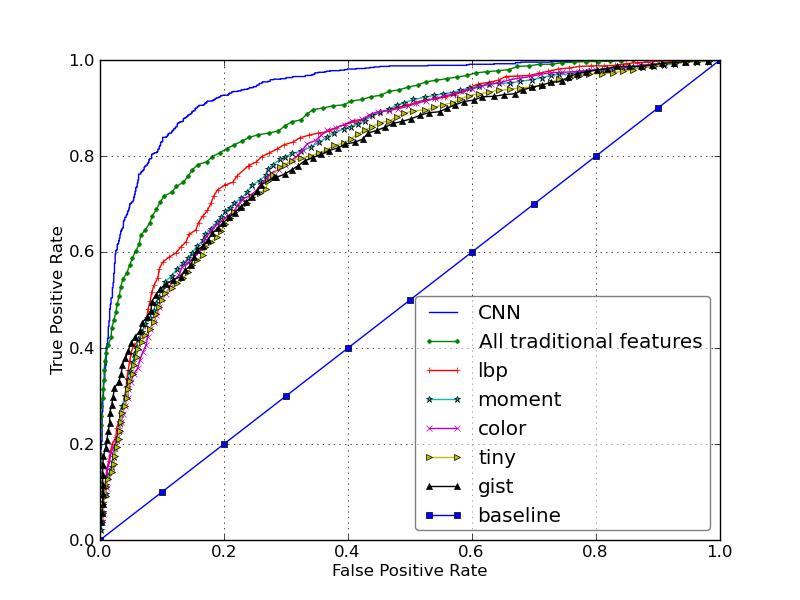
\includegraphics[width=0.4\textwidth]{figs/ROC-CNN-curves.jpg} &
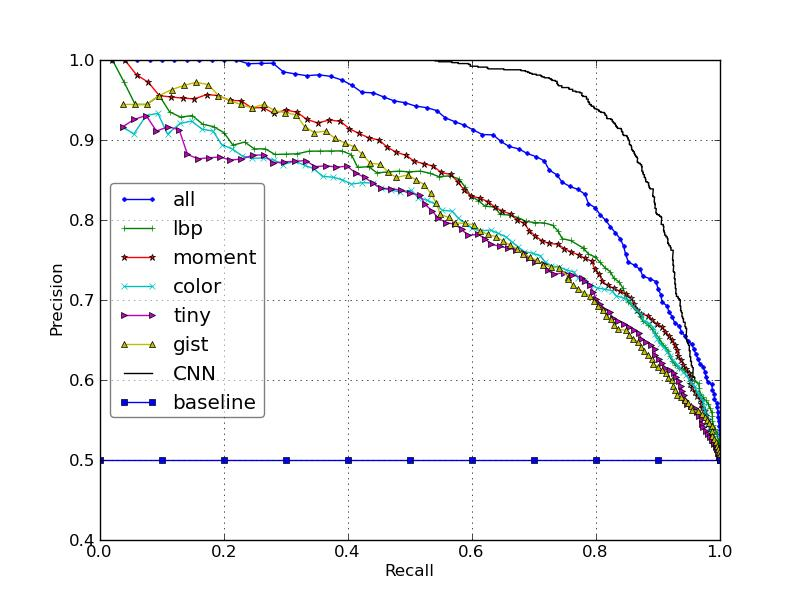
\includegraphics[width=0.4\textwidth]{figs/PR-CNN-curves.jpg} \\
\end{tabular}
\end{center}
\vspace{-8pt}
\caption{
Snow classification results for different features and combinations, in terms of {\textit{(left):}} ROC curves for the task of classifying snow vs. non-snow images; and 
{\textit{(right):}} Precision-Recall curves for the task of retrieving snow images.
}
\label{fig:PR_ROC_snow}
\end{figure*}
%
%\begin{table}
%\begin{center}
%{\footnotesize{
%\begin{tabular}{|l|c|c|}
%\hline 
%Feature & Kernel  & Accuracy\tabularnewline
%\hline 
%\hline 
%Random Baseline  & --- & 50.0\%\tabularnewline
%\hline 
%\hline
%Gist & RBF & 73.7\%\tabularnewline
%\hline 
%Color  & $\chi^2$ & 74.1\%\tabularnewline
%\hline
%Tiny & RBF & 74.3\%\tabularnewline
%\hline 
%Spatial Color Moments & RBF & 76.2\%\tabularnewline
%\hline 
%Spatial pyramid LBP & RBF &\textbf{77.0\%}\tabularnewline
%\hline 
%\hline
%All features  & linear & \textbf{80.5\%}\tabularnewline
%\hline 
%CNN& -& \textbf{88.06\%}\tabularnewline
%\hline
%\end{tabular}
%}}
%\caption{Performance of different features  for snow detection, all using SVMs for classification. }
%\label{tab:snow}
%\end{center}
%\end{table}

\begin{table}\centering
\ra{1.3}
\caption{\textbf{Performance of different features  for snow detection, all using SVMs for classification.} }
\label{tab:snow}
\begin{tabular}{@{}lcr@{}}\toprule
Feature & Kernel & Accuracy\\\midrule
Random Baseline  & --- & 50.00\%\\
Gist & RBF & 73.70\%\\
Color  & $\chi^2$ & 74.10\%\\
Tiny & RBF & 74.30\%\\
Spatial Color Moments & RBF & 76.20\%\\
Spatial pyramid LBP & RBF &\textbf{77.00\%}\\\midrule
All features  & linear & \textbf{80.50\%}\\
CNN& -& \textbf{88.06\%}\\
\bottomrule\\
\end{tabular}
\end{table}

The best performance we had using our traditional visual features using SVM is 80.5\% accuracy.  We also build CNN visual model for snow using Imagenet pre-trained model. We fine-tune our model using our training data. CNN  achieves 88\% accuracy which  outperforms all other features by 7.44\% . Therefore, we used CNN as our visual model for final predictions.  Similar to visual model we also build SVM using only tags as features and our text classifier achieves 87\% accuracy.




We now turn to presenting experimental results for estimating the
geo-temporal distributions of snow.

\subsubsection{Snow prediction on cities}


We first test how well the Flickr data can predict snowfall at a local
level, and in particular for cities in which high-quality
surface-based snowfall observations exist and for which photo density is high.

We choose 4 U.S. metropolitan areas, New York City, Boston, Chicago and
Philadelphia, and try to predict both daily snow presence as well as
the quantity of snowfall.  For each city, we define a corresponding
geospatial bounding box and select the NOAA ground observation stations in that area. 
For example, 
Figure~\ref{tab:city_statistics} shows the the stations 
and the bounding box for 
New York City. We calculate the ground truth daily snow quantity for a city as the average of
the valid 
snowfall values from its stations.

We call any day with a non-zero snowfall or snowcover to be a snow day,
and any other day to be a non-snow day.

Figure~\ref{tab:city_statistics} also presents some basic statistics for
these 4 cities.  All of our experiments involve 4 years (1461 days) of
data from January 2007 through December 2010; we reserve the first two
years for training and validation, and the second two years for
testing.


\begin{figure}
\begin{center}
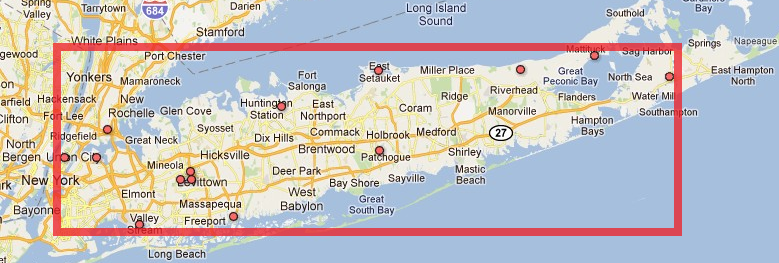
\includegraphics[width=0.35\textwidth]{plots/nyc_stations.png} 
\end{center}
\begin{center}
{\small{
\newcommand{\spc}{\hspace{2pt}}
%\begin{tabular} {|@{\spc}l@{\spc}|@{\spc}r@{\spc}|@{\spc}r@{\spc}|@{\spc}r@{\spc}|@{\spc}r@{\spc}|} 
%\hline 
%\textbf{} &{NYC}  &{Chicago} &{Boston}&{Philadelphia} \tabularnewline
%\hline 
%{Mean active Flickr users / day} &{65.6} &{94.9} &{59.7} &{43.7} \tabularnewline
%\hline 
%{Approx. city area ($km^2$)} &{3,712} &{11,584} &{11,456} &{9,472}  \tabularnewline
%\hline 
%{User density (avg users/unit area)} &{112.4} &{52.5} &{33.5} &{29.6} \tabularnewline
%\hline 
%{Mean daily snow (inches)} &{0.28} &{0.82} &{0.70} &{0.35} \tabularnewline
%\hline 
%{Snow days (snow>0 inches)} &{185} &{418} &{373} &{280} \tabularnewline
%\hline 
%{Number of obs. stations} &{14} &{20} &{41} &{26} \tabularnewline
\ra{1.3}
\begin{tabular}{@{\spc}l@{\spc}|@{\spc}r@{\spc}|@{\spc}r@{\spc}|@{\spc}r@{\spc}|@{\spc}r@{\spc}}\toprule
\textbf{} &{NYC}  &{Chicago} &{Boston}&{Philly} \\\midrule 
{Mean active Flickr users / day} &{65.6} &{94.9} &{59.7} &{43.7} \\
{Approx. city area ($km^2$)} &{3,712} &{11,584} &{11,456} &{9,472}  \\
{User density (avg users/unit area)} &{112.4} &{52.5} &{33.5} &{29.6} \\
{Mean daily snow (inches)} &{0.28} &{0.82} &{0.70} &{0.35} \\
{Snow days (snow$>$0 inches)} &{185} &{418} &{373} &{280} \\
{Number of obs. stations} &{14} &{20} &{41} &{26} \\
\bottomrule
\end{tabular}}}
\end{center}
\vspace{-12pt}
 \caption {\textit{Top:} New York City geospatial bounding box used to select Flickr photos, and locations of NOAA observation stations. \textit{Bottom:} Statistics about spatial area, photo density, and ground truth for each of the 4 cities.}
\label{tab:city_statistics} 
\end{figure}




\xhdr{Daily snow classification for 4 cities.}
Figure~\ref{fig:city_roc}(a) presents ROC curves for this
daily snow versus non-snow classification task on New York City. The figure compares the likelihood
ratio confidence score from equation~(\ref{eq:conf}) to the baseline
approaches (voting and percentage), using the tag set
${\cal S}$=\{snow, snowy, snowing, snowstorm\}.
The area under the ROC curve (AUC) statistics are 0.929, 0.905, and 0.903 for confidence, percentage, and voting, respectively, 
and the improvement of the confidence method is statistically significant 
with $p=0.0713$ according to the statistical test of~\cite{auc}.
The confidence method also outperforms other methods for the other three cities (not shown due to
space constraints).  ROC curves for all 4 cities using the likelihood
scores are shown in Figure~\ref{fig:city_roc}(b). Chicago has the best
performance and Philadelphia has the worst; a possible explanation
is that Chicago has the most active Flickr users per
day (94.9) while Philadelphia has the least (43.7).

These methods based on presence or absence of tags are simple and very
fast, but they have a number of disadvantages, including that the tag
set must be manually chosen and that negative correlations between
tags and phenomena are not considered.
We thus tried training a classifier to learn these relationships automatically.
For each day in each city, we produce a single binary feature vector indicating whether 
or not a given tag was used on that day. Also we tried to build classifiers trained based on our likelihood ratio computed based on tags or our visual model predictions. Table~\ref{tab:city_conf_tag_vision} shows the results foe these classifiers. Best prefromance obtained when we combine the confidence scores of tags and visual model based on CNN.
%
%\begin{figure*}[th!]
%\begin{center}
%\vspace{-16pt}
%\begin{tabular}{cc}
% 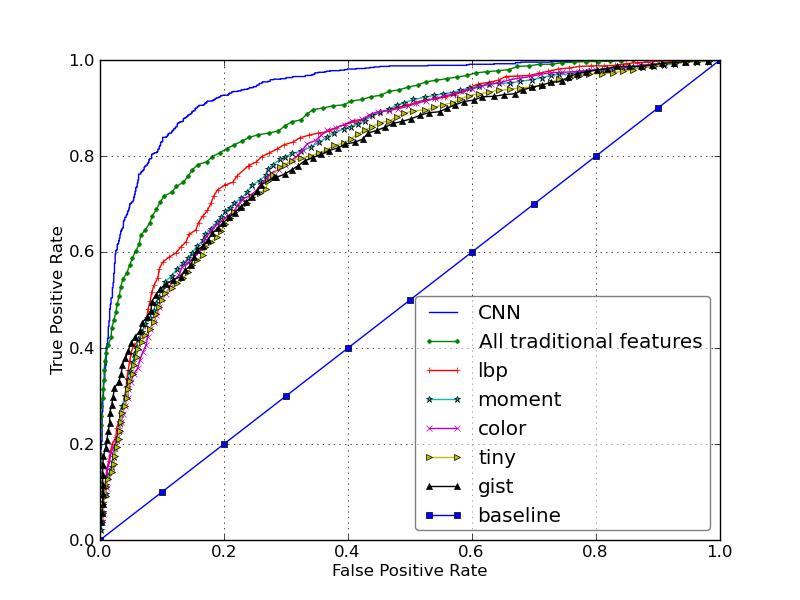
\includegraphics[width=0.4\textwidth]{figs/ROC-CNN-curves.jpg} &
%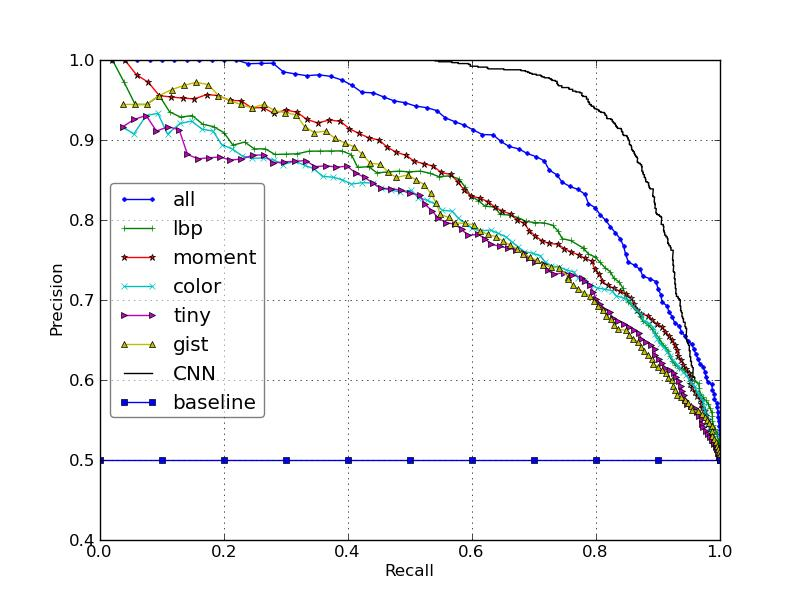
\includegraphics[width=0.4\textwidth]{figs/PR-CNN-curves.jpg} \\
%\end{tabular}
%\end{center}
%\vspace{-8pt}


\begin{figure*}
\begin{center}
\hspace{-0.25in}
\small{
\begin{tabular}{cc}
%{@{}c@{}c@{}c@{}c@{}}
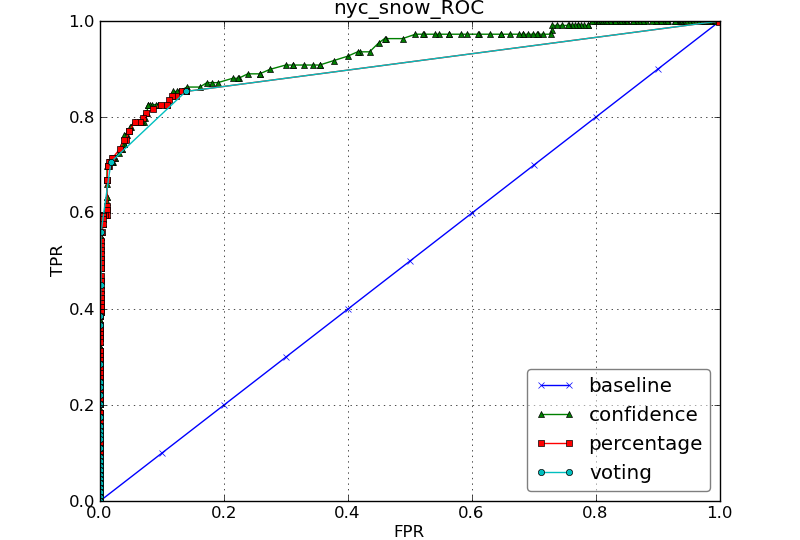
\includegraphics[width=0.40\textwidth,clip,trim=0.4in 0 0.8in 0]{plots/nyc_snow_ROC.png} &
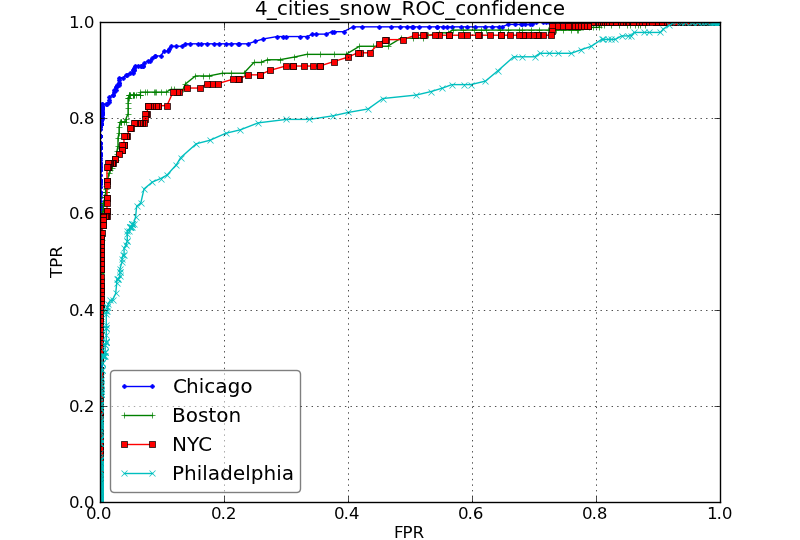
\includegraphics[width=0.40\textwidth,clip,trim=0.4in 0 0.8in 0]{plots/city_cmp_snow_ROC.png} \\
(a) & (b)  
\end{tabular}
}
\end{center}
\vspace{-6pt}
\caption{ROC curves for binary snow predictions: (a) ROC curves for New York City, comparing likelihood
ratio confidence score to voting and percentage approaches, (b) ROC curves for 4 cities using the likelihood
scores}
\label{fig:city_roc}
\vspace{-6pt}
\end{figure*}








%\begin{table*} 
% \caption {\textbf{Results for Confidence score model using tags and visual classifiers for our 4 cities .}}
%\label{tab:city_conf_tag_vision} 
%\begin{center}
%{
%\begin{tabular} {|c|c|c|c|c|c|} 
%\hline 
%City &  baseline & tags  &  tag confidence  &  vision conf & tags conf and vision conf \tabularnewline
%\hline 
%
%{NYC} & 85\% & 85.75 \% &90.4241 \%&90.2873 \% &92.3393 \%\tabularnewline
%\hline 
%{Chicago)} &72.80\% & 93.5616 \% &94.1176 \% &93.1601 \% &95.0752 \%  \tabularnewline
%\hline 
%{Boston} & 75.60\%& 90.5479 \% &89.1781 \%&85.2055 \% & 91.2329 \% \tabularnewline
%\hline 
%{Philly} & 80.50\% & 85.34\% & 89.1929 \% &85.0889 \%	 & 89.1929 \%  \tabularnewline
%\hline 
%
%\end{tabular}}
%\end{center}
%\vspace{-12pt}
%\end{table*}

\begin{table*}\centering
\ra{1.3}
\caption {\textbf{Results for Confidence score model using tags and visual classifiers for our 4 cities .}}
\label{tab:city_conf_tag_vision} 
\begin{tabular}{@{}crrrrr@{}}\toprule
City &  baseline & tags  &  tag confidence  &  vision conf & tags conf and vision conf \\\midrule
{NYC} & 85\% & 85.75 \% &90.42 \%&90.28 \% &92.33 \%\\
{Chicago} &72.80\% & 93.56 \% &94.11 \% &93.16 \% &95.07 \%  \\
{Boston} & 75.60\%& 90.54 \% &89.17 \%&85.20 \% & 91.23 \% \\
{Philly} & 80.50\% & 85.34\% & 89.19 \% &85.08 \%	 & 89.19 \%  \\
\bottomrule
\end{tabular}
\vspace{-12pt}
\end{table*}

\subsubsection{{Continental-scale snow prediction}}
Predicting snow for individual cities is of limited practical use because accurate meteorological data already exists for these highly populated areas.
Here we ask whether phenomena can be
monitored at a continental scale, a task for which existing data
sources are less complete and accurate.  We use the photo data and
ground truth described in Section~\ref{sec:results}, although for the
experiments presented in this paper we restrict our dataset to North
America (which we defined to be a rectangular region spanning from 10
degrees north, -130 degrees west to 70 degrees north, -50 degrees
west). (We did this because Flickr is a dominant photo-sharing site in
North America, while other regions have other popular
sites --- e.g. Fotolog in Latin America and Renren in China.)  

The spatial resolution of the NASA satellite ground truth datasets is 0.05 degrees
latitude by 0.05 degrees longitude, or about $5 \times 5 km^2$ at the
equator.  (Note that the surface area of these bins is
non-uniform because lines of longitude get closer together near the
poles.)  However, because the number of photos uploaded to Flickr on
any particular day and at any given spatial location is relatively
low, and because of imprecision in Flickr geo-tags, we produce
estimates at a coarser resolution of 1 degree square, or roughly $100
\times 100 km^2$. To make the NASA maps comparable, we downsample them
to this same resolution by averaging the high confidence observations within the coarser bin.
%We then threshold the confidence and snow cover percentages to annotate
%each bin with one of three ground truth labels: 
%%
%\begin{packed_itemize}
%\item[---] Snow bin, if confidence is above 90 and coverage above 80,
%\item[---] Non-snow bin, if confidence is above 90 and coverage is 0,
%\item[---] Unknown bin, otherwise.
%\end{packed_itemize}
%%

%Figure ~\ref{fig:snowcurve} shows the precision and recall curve of snow prediction in continental-scale.
% bar plot of 2 places
\begin{figure*}
%{\small{
\begin{center}

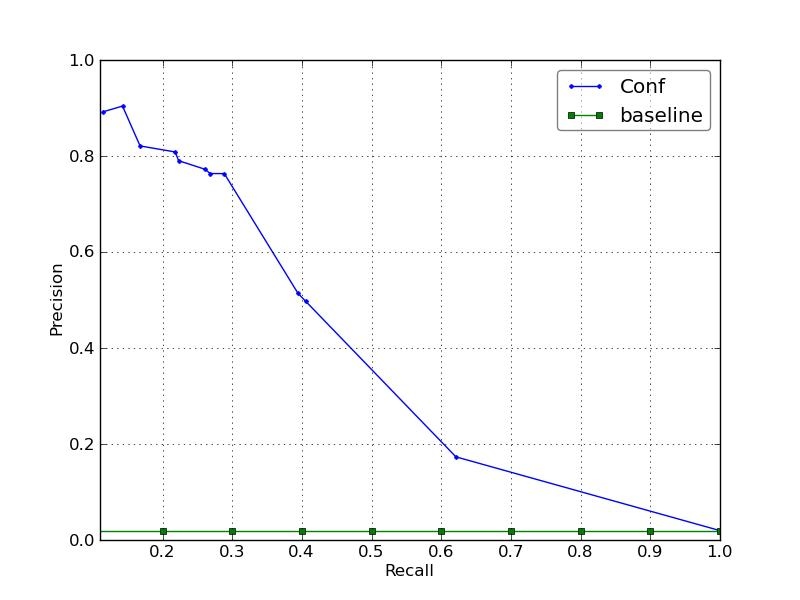
\includegraphics[width=0.40\textwidth,clip,trim=0.4in 0 0.8in 0]{figs/PR-snow.jpg}
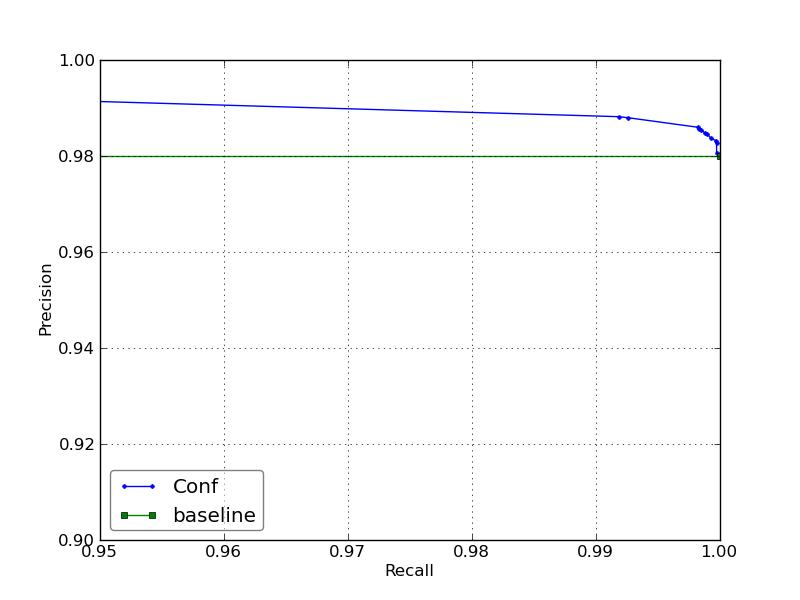
\includegraphics[width=0.40\textwidth,clip,trim=0.4in 0 0.8in 0]{figs/PR-nonsnow.jpg}
%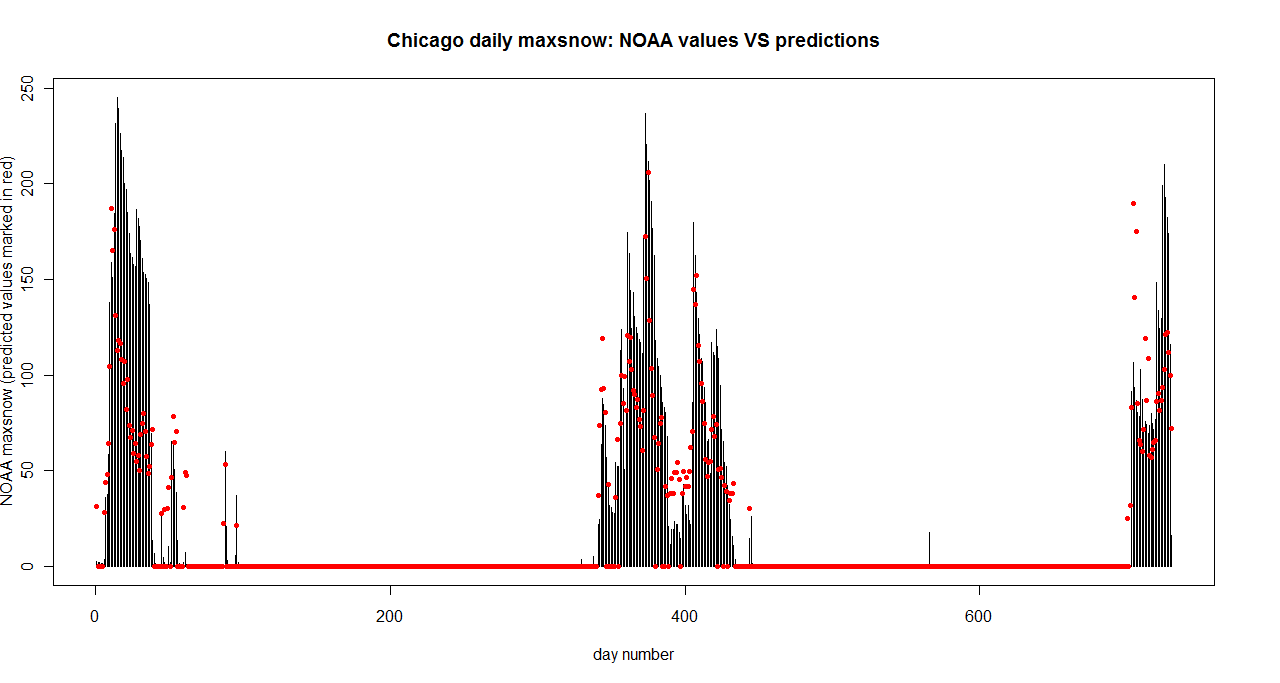
\includegraphics[width=0.5\textwidth,height=1.4in,clip,trim=0 0.5in 0in 0.6in]{plots/chicago_noaa_vs_prediction_prev_3.png} 

\end{center}
%}}
\vspace{-24pt}
\caption{Precision and recall curve of snow prediction (left) and nonsnow (right) in continental scale.}
\label{fig:snowcurve}
\vspace{-12pt}
\end{figure*}

% bar plot of 2 places
%\begin{figure}
%%{\small{
%\begin{center}
%
%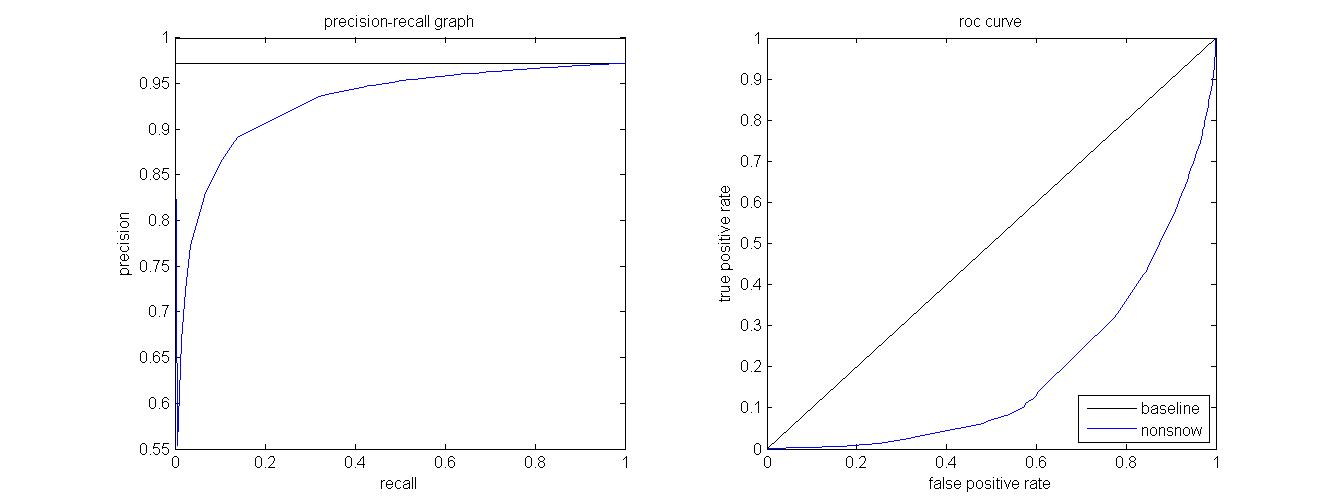
\includegraphics[width=0.5\textwidth]{nonsnowcurve.jpg}
%
%%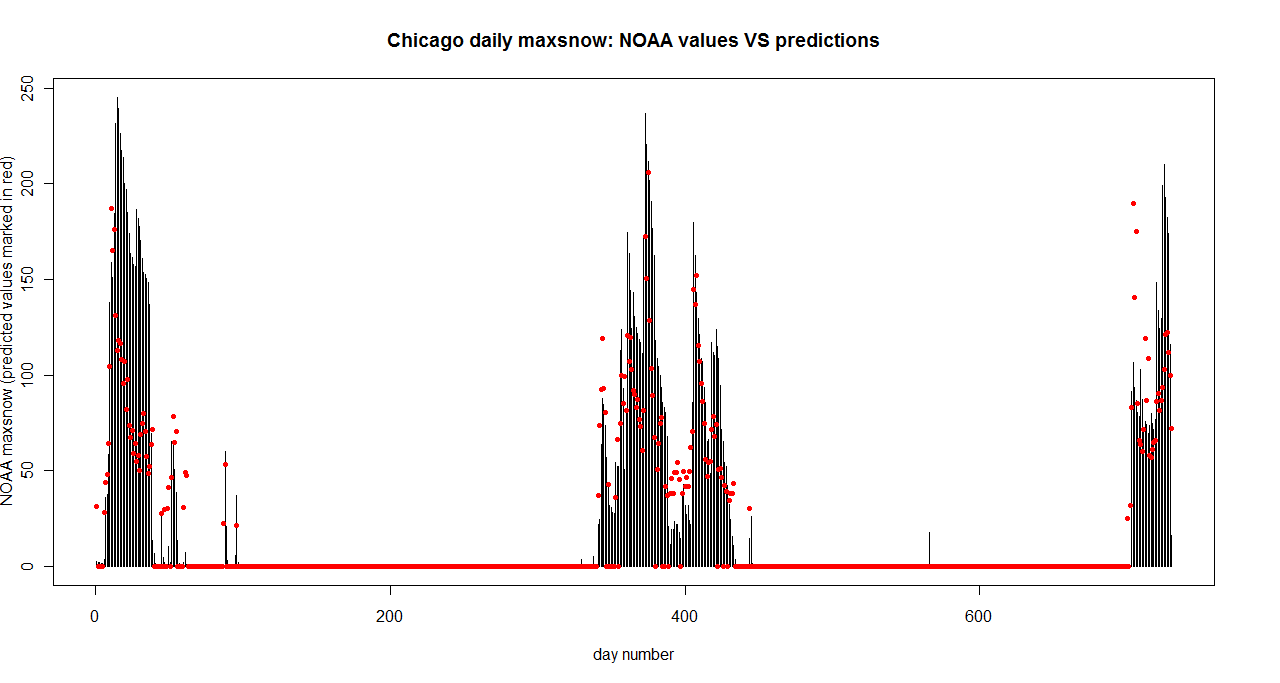
\includegraphics[width=0.5\textwidth,height=1.4in,clip,trim=0 0.5in 0in 0.6in]{plots/chicago_noaa_vs_prediction_prev_3.png} 
%
%\end{center}
%%}}
%\vspace{-24pt}
%\caption{Precision and recall curve of nonsnow prediction in continental scale.}
%\label{fig:nonsnowcurve}
%\vspace{-12pt}
%\end{figure}
Figure ~\ref{fig:snowcurve} shows the precision and recall curve of snow prediction in continental-scale.
Here we limit our predictions for the bins which have photos taken at that time and location, we do this by keeping the bins have ground truth and photos at the same time. 
We computed our confidence scores based on tags and image-classification, then we trained simple decision tree to learn the correct thresholds to make final prediction. We achieve almost 0.5\% over the baseline (cutting the error rate by more than 20\%), the baseline in our case is the majority class which predicts now snow all the time.  
  

%increases over the baseline (98.0\% - majority class which predicts now snow all the time).   


%We achieve 98.4\% by combining likelihood scores for tags and visual features compare to the 98.0\% for majority class classifier in this case. We cutting the error rate by more than 20%  


\subsection{Vegetation case}

\subsubsection{Single image classification}


Using the method we describe in Section~\ref{sec:method}, we train and test the vision model on our hand-labeled data set.
There are 4000 images in training set and 2000 images in testing set. In both training and testing set, the number of positive and negative images are the same. Here we present the results on image classification level.

%\subsubsection{not using tag in vegetation case}
%
%We tested the performance of using only tags to make vegetation coverage prediction. The performance shows tag
%feature is not going to improve the result of using visual evidence.
%
%%%%%%%%%%%%    why this part     %%%%%%%%%%%%%%%%%
%%This is the result of vegetation case in www paper.
%%I guess this might help us to explain why we don't use tag in vege case in this paper.
%%%%%%%%%%%%%%%%%%%%%%%%%%%%%%%%%%%%%

%\begin{table} 
% \caption {\textbf{Results for our  visual models for vegetation.}}
%\label{tab:veg_img_classifier} 
%\begin{center}
%{
%\begin{tabular} {|c|c|} 
%\hline 
%Visual feature &  Accuracy \tabularnewline
%\hline 
%\hline
%Random Baseline & 50.00\%\tabularnewline
%\hline
%\hline
%Color SIFT & 78.10\%\tabularnewline
%\hline 
%Color GIST & 82.58\% \tabularnewline
%\hline 
%\hline
%SIFT and GIST& 85.9\% \tabularnewline
%\hline 
%CNN\% &  88.0\%\tabularnewline
%\hline 
%\end{tabular}
%}
%\end{center}
%\end{table}

\begin{table}\centering
\ra{1.3}
\caption {\textbf{Results for our  visual models for vegetation.}}
\label{tab:veg_img_classifier} 
\begin{tabular}{@{}cr@{}}\toprule
Visual feature &  Accuracy\\\midrule
Random Baseline & 50.00\%\\
Color SIFT & 78.10\%\\
Color GIST & 82.58\% \\
SIFT and GIST& 85.90\% \\
CNN\% &  88.00\%\\
\bottomrule
\end{tabular}
\end{table}


\subsubsection{Vegetation coverage over time and space}
We consider north America area has more images uploaded to photo-sharing website, and is also where Ecologists in the US would be interested in the changing color of vegetation. 
%In our work, we define north America as latitude 10$^{\circ}$ to 70$^{\circ}$ and longitude -130$^{\circ}$ to -50$^{\circ}$.


We combine all the evidence over space and time in North America from 2007 to 2010. We compute confidence score described in Section~\ref{sec:method}. 
%Confidence score is measuring the ratio of log likelihood of being a vegetation bin or not at each time period. All the prior statistics are learnt from satellite ground truth in 2007 and 2008.
The prior probability of a place being covered by vegetation at some time is 75.2\%.
%(I doubt this number. This is because the ground truth put too many bins in gray area while there are too many non-green bins on the north that we don't really care.) 
For an image taken from a place covered by green vegetation at that time, the probability of this image being a green image is 27.18\%. On the other hand, it's only 3.03\% probability to see a green image in a place not covered by enough green vegetation at that time.

%Now we present the performance of vegetation detection in north America.

%\hfill \break
%\hfill \break
While the satellite has ground truth for 87594 bins in North America, our method predicts 61602 bins (70.3\% in quantity). Moreover, about 20\% of satellite ground truth locate in north Canada. On the other hand, our data is from users in social media. So our prediction focus on more populated locations or places people like to visit such as natural scenery.

In North America, the overall accuracy of our method is 93.2\% comparing to the 86.6\% majority baseline. The precision of green bins is 98.8\% and the precision of non-green bins is 68.2\%. Recall of green bins is 93.3\% and recall of non-green bins is 92.5\%. We tested the performance of using only tags to make vegetation coverage prediction ~\cite{ecology2012www}. The performance shows tag
feature is not going to improve the result of using visual evidence.


%snowcurve.pdf
%curvevege.jpg
% precision-recall of vege
Figure ~\ref{fig:curvevege} shows the precision and recall curve of snow prediction in continental-scale.
% bar plot of 2 places
\begin{figure*}
%{\small{
\begin{center}

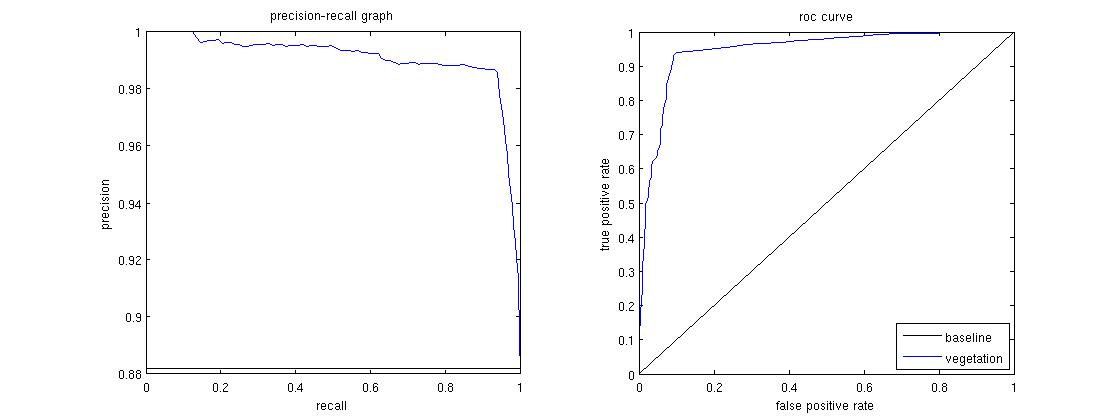
\includegraphics[width=0.80\textwidth]{curvevege.jpg}

%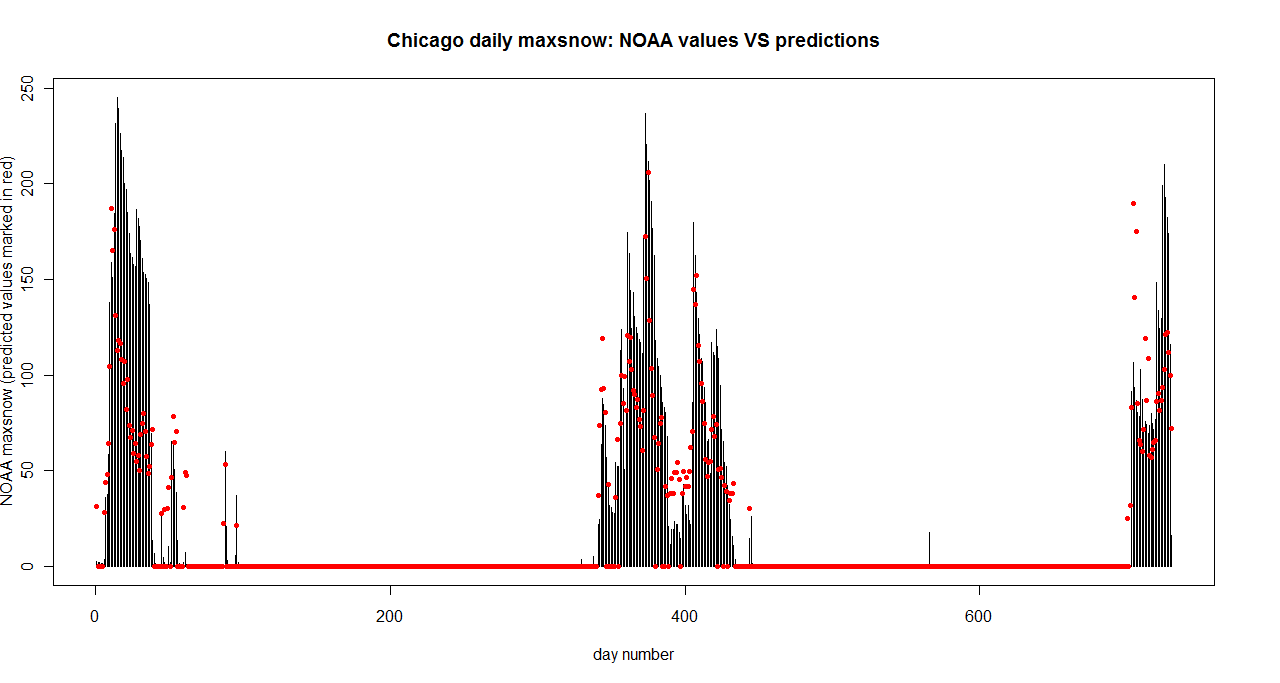
\includegraphics[width=0.5\textwidth,height=1.4in,clip,trim=0 0.5in 0in 0.6in]{plots/chicago_noaa_vs_prediction_prev_3.png} 

\end{center}
%}}
\vspace{-24pt}
\caption{Precision and recall curve of vegetation prediction in continental scale.}
\label{fig:curvevege}
\vspace{-12pt}
\end{figure*}

%
%# of bins gt shows nongreen = 67571
%overlap of gt and predi both shows nongreen = 1085
%accuracy = 0.016057184295
%# of bins predi shows green = 42317
%overlap of gt and predi both shows green = 7061
%accuracy = 0.166859654512
%# of bins that both have data = 8741
%overlap = 8146
%accuracy = 0.931929985128
%# of bins that predi have data = 61602
%# of bins that gt have data = 87594
%ratio = 0.703267347079
%in bins both have data, # of predi as gr = 7149
%overlap = 7061
%precision of gr = 0.987690586096
%in bins both have data, # of predi as nongr = 1592
%overlap = 1085
%precision of nongr = 0.681532663317
%in bins both have data, # of gt as gr = 7568
%overlap = 7061
%recall of gr = 0.933007399577
%in bins both have data, # of gt as nongr = 1173
%overlap = 1085
%recall of nongr = 0.924978687127
%
%
%baseline = 0.865804827823


%
%***confusion matrix maps and data
%
%\begin{table}[b]
%\begin{center}
%{\footnotesize{
%\begin{tabular}{|l|c|c|}
%\hline 
%--- & \multicolumn{2}{c|}{Ground truth}\tabularnewline
%\hline
%--- & Greenery & Non-Greenery\tabularnewline
%\hline 
%\hline 
%%Random Baseline  & --- & 50.0\%\tabularnewline
%%\hline 
%%\hline
%Greenery & 2580 & 36\tabularnewline
%\hline 
%Non-Greenery & 353 & 400\tabularnewline
%\hline
%\end{tabular}
%}}
%\caption{Confusion matrix of vegetation detection in 2007}
%\label{tab:confusionmatrix}
%\end{center}
%\end{table}
%(This table looks terrible. Hope there is a way to make it prettier.)
%(??? Result is presented in video. Is a map necessary here? or a better way?)


\begin{figure*}[th]
{\small{
\begin{center}
\begin{tabular}{@{}c@{\,\,\,}c@{\,\,\,}c@{\,\,\,}c@{\,\,\,}c@{\,\,\,}}
%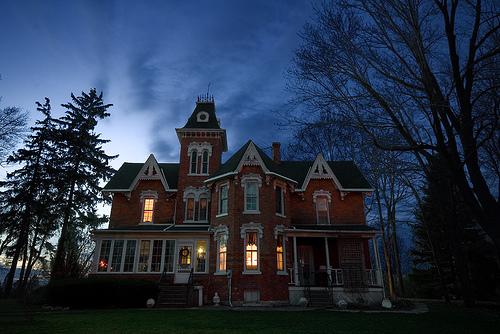
\includegraphics[width=0.19\textwidth]{imggrid/falseposi/1.jpg} &
%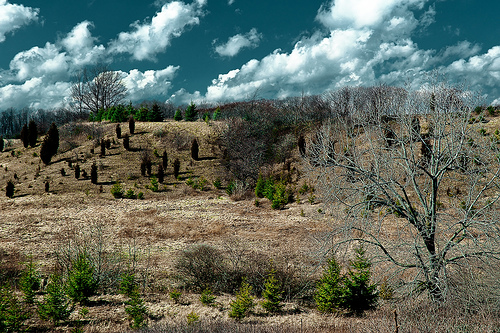
\includegraphics[width=0.19\textwidth]{imggrid/falseposi/2.jpg} &
%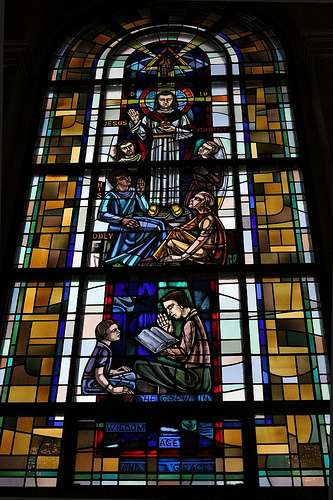
\includegraphics[height=1in]{imggrid/falseposi/3.jpg} &
%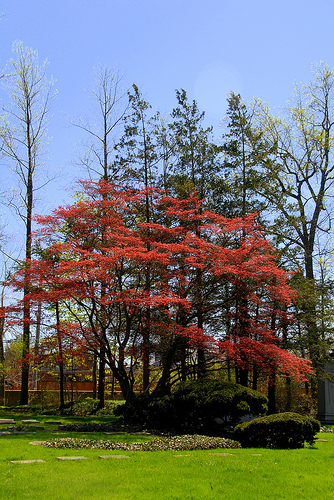
\includegraphics[height=1in]{imggrid/falseposi/4.jpg} &
%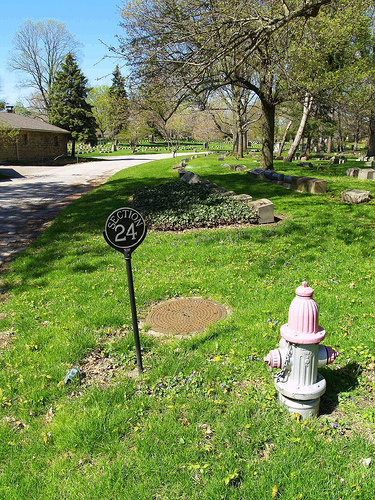
\includegraphics[height=1in]{imggrid/falseposi/5.jpg} \\
%%\multicolumn{5}{c}{(a) Random positive images in vegetation dataset} \\
%\\[-6pt]
%\hline
%\\[-6pt]
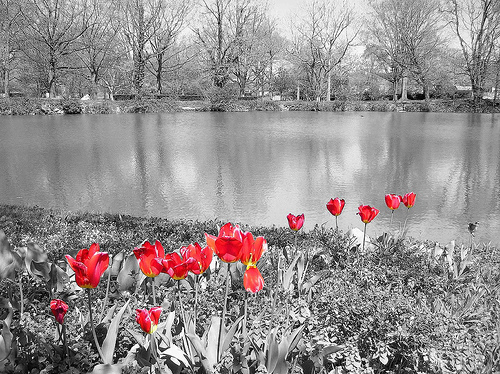
\includegraphics[width=0.19\textwidth]{imggrid/falseposi/6.jpg} &
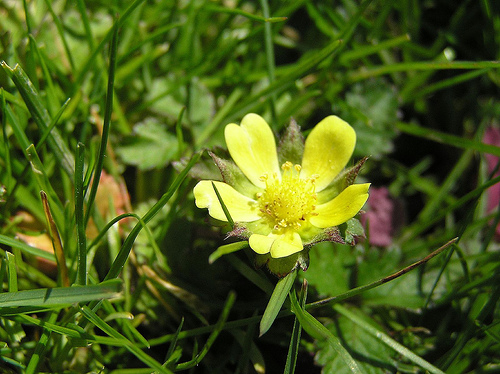
\includegraphics[width=0.19\textwidth]{imggrid/falseposi/7.jpg} &
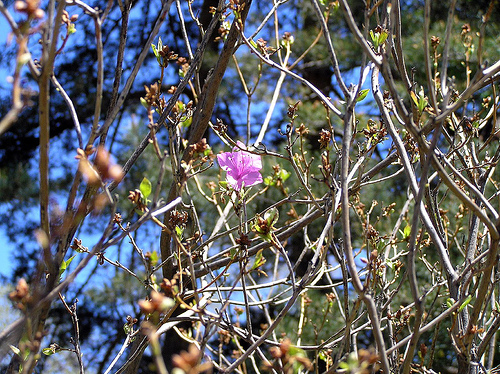
\includegraphics[width=0.19\textwidth]{imggrid/falseposi/8.jpg} &
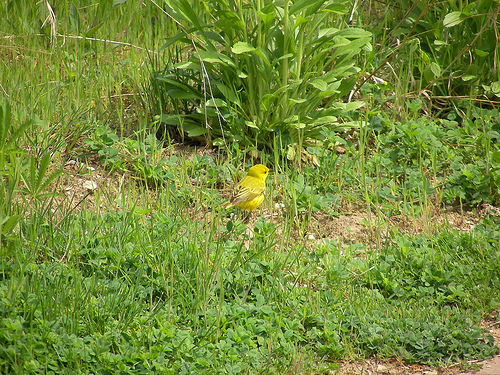
\includegraphics[width=0.19\textwidth]{imggrid/falseposi/9.jpg} &
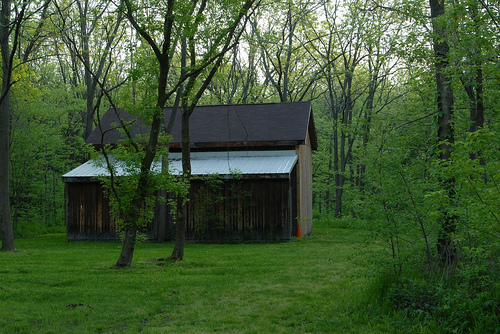
\includegraphics[width=0.19\textwidth]{imggrid/falseposi/10.jpg} \\
%\multicolumn{5}{c}{(a) Random positive images in vegetation dataset} \\ 
\\[-6pt]
\hline
\\[-6pt]
%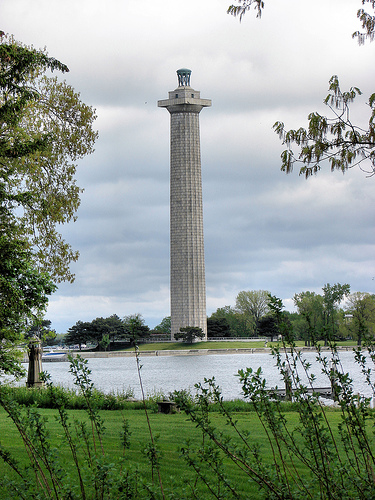
\includegraphics[height=1in]{imggrid/falseposi/11.jpg} &
%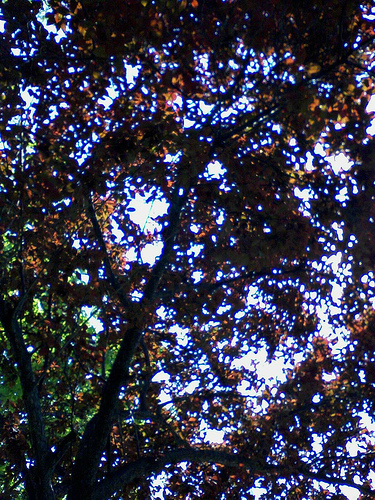
\includegraphics[height=1in]{imggrid/falseposi/12.jpg} &
%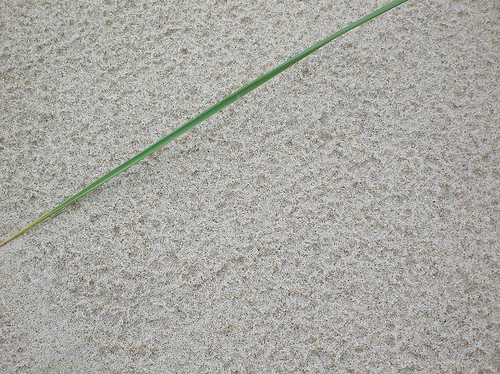
\includegraphics[width=0.19\textwidth]{imggrid/falseposi/13.jpg} &
%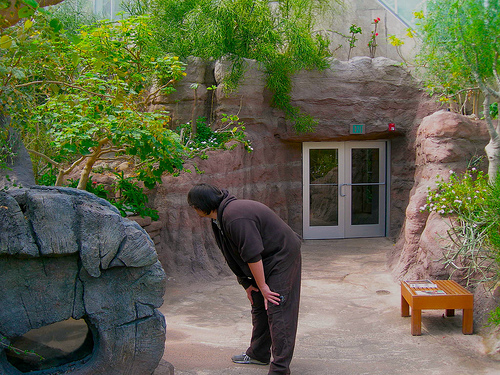
\includegraphics[width=0.19\textwidth]{imggrid/falseposi/14.jpg} &
%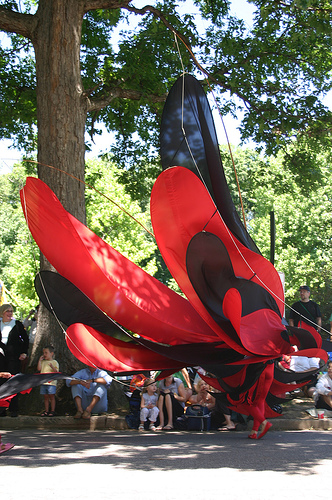
\includegraphics[height=1in]{imggrid/falseposi/15.jpg} \\
%%\multicolumn{5}{c}{(c) Random false negatives (snow images classified as non-snow)} \\ 
%\\[-6pt]
%\hline
%\\[-6pt]
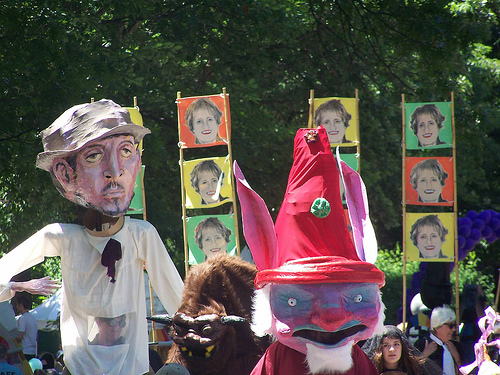
\includegraphics[width=0.19\textwidth]{imggrid/falseposi/16.jpg} &
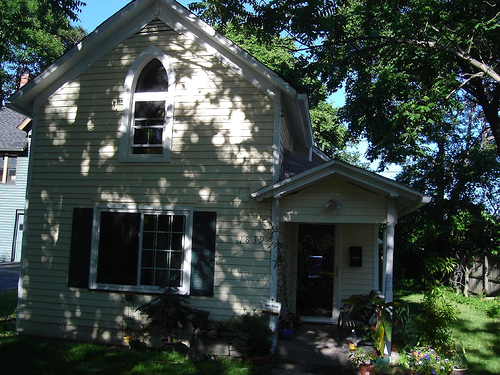
\includegraphics[width=0.19\textwidth]{imggrid/falseposi/17.jpg} &
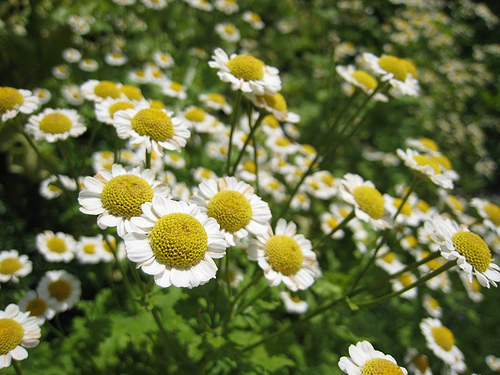
\includegraphics[width=0.19\textwidth]{imggrid/falseposi/18.jpg} &
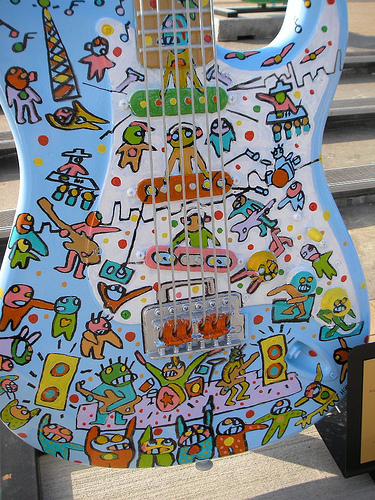
\includegraphics[height=1in]{imggrid/falseposi/19.jpg} &
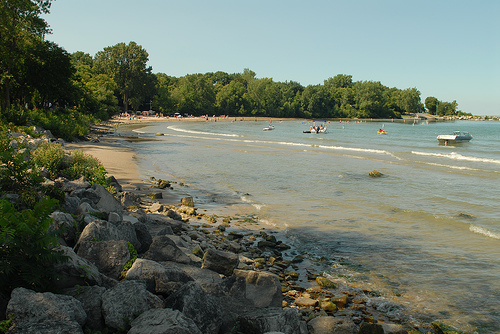
\includegraphics[width=0.19\textwidth]{imggrid/falseposi/20.jpg} \\
%\multicolumn{5}{c}{(b) Random negative images in vegetation dataset} \\
\end{tabular}
\end{center}
}}
\caption{In vegetation detection over North America in 2009 and 2010, among all false positive bins, there are ... images that are predicted as greenery. And these images are the reason these bins are predicted as green. Here are some random selected examples of the green images.}
\label{fig:falseposi}
\end{figure*}

%****explain errors

Generally, all the false negative error is due to the sparseness of data. While not enough images are collected at certain location during some time, there is either no green image found or green images are too few compare to the quantity of non-green images. On the other hand, false positive error is rare (less than 1\%) and complex. We found most images in the false positive bins are actually green vegetation images. ( here we need some more explanation) In figure ~\ref{fig:falseposi}, we show some examples of images in false positive bins.



\subsubsection{Performance at single place over time}
For each single location, we can find out when exactly did the leaves turn yellow as well as when
did the leaves turn back to green. 
Figure ~\ref{fig:placeinbar} shows vegetation coverage of 6 places over 2009 and 2010. 
Prediction results on top usually have more data available than groud truth on the bottom. 
And we can see the ground truth is likely missing at the time when the leaves change color. 

% bar plot of 2 places
\begin{figure}
%{\small{
\begin{center}
\begin{tabular}{ccc}
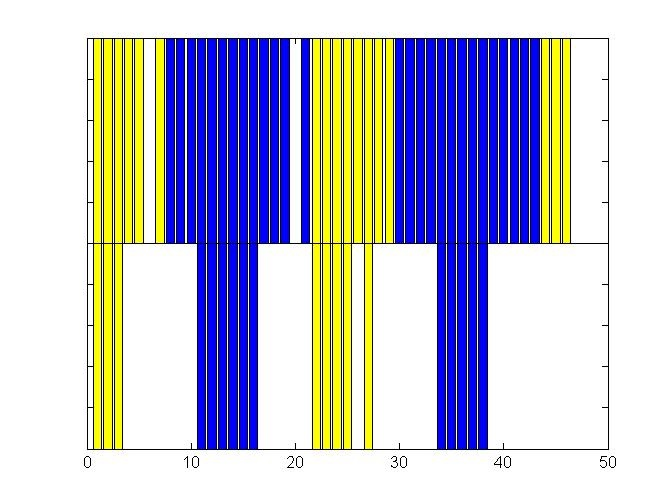
\includegraphics[width=0.14\textwidth]{bar/8560.jpg} &
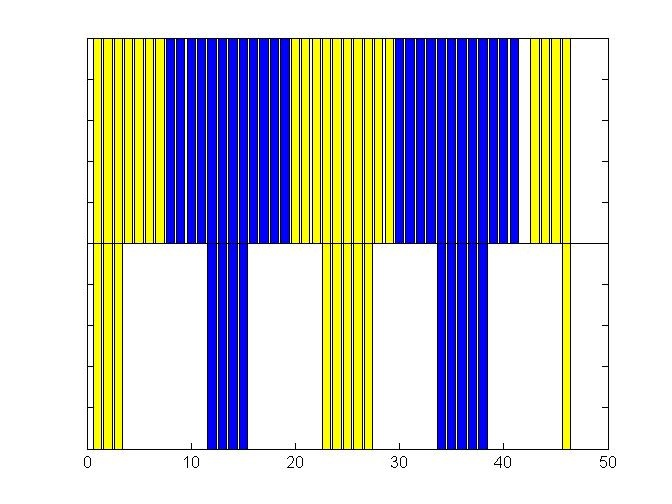
\includegraphics[width=0.14\textwidth]{bar/8561.jpg} &
%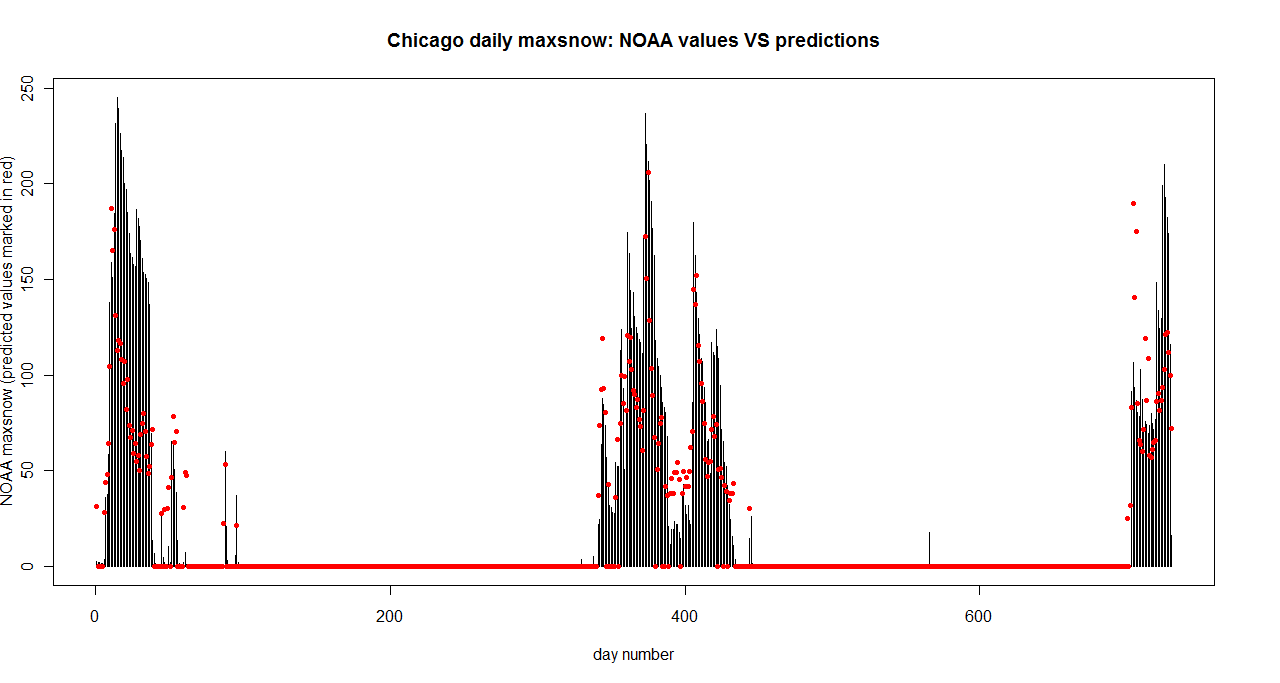
\includegraphics[width=0.5\textwidth,height=1.4in,clip,trim=0 0.5in 0in 0.6in]{plots/chicago_noaa_vs_prediction_prev_3.png} 
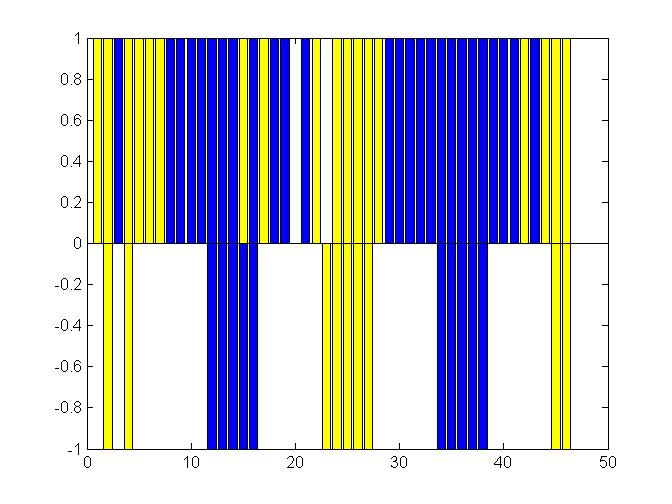
\includegraphics[width=0.14\textwidth]{bar/8881.jpg} \\
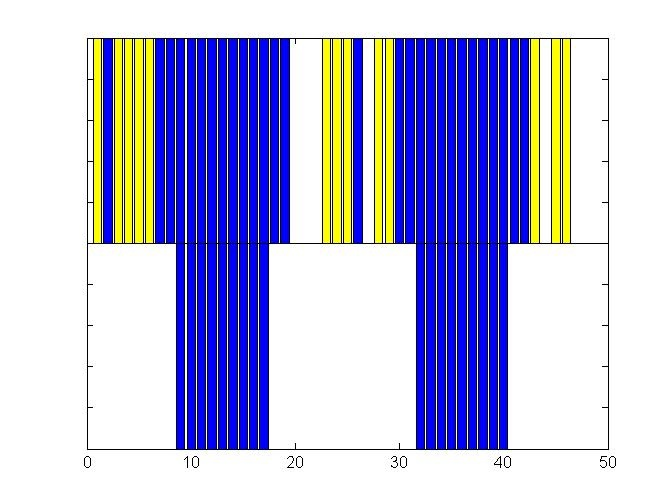
\includegraphics[width=0.14\textwidth]{bar/8911.jpg} &
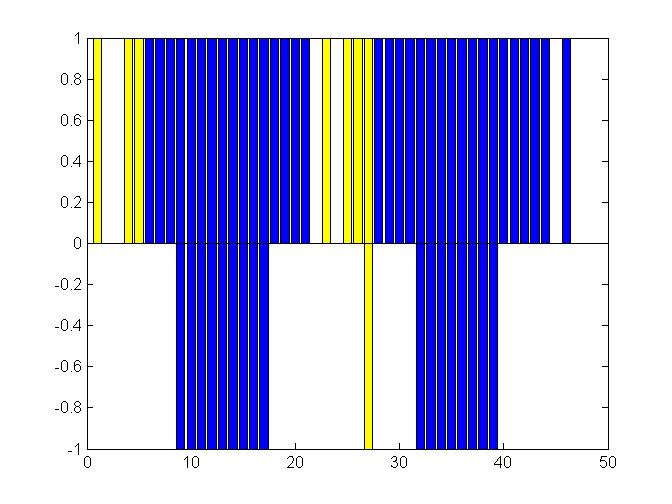
\includegraphics[width=0.14\textwidth]{bar/9705.jpg} &
%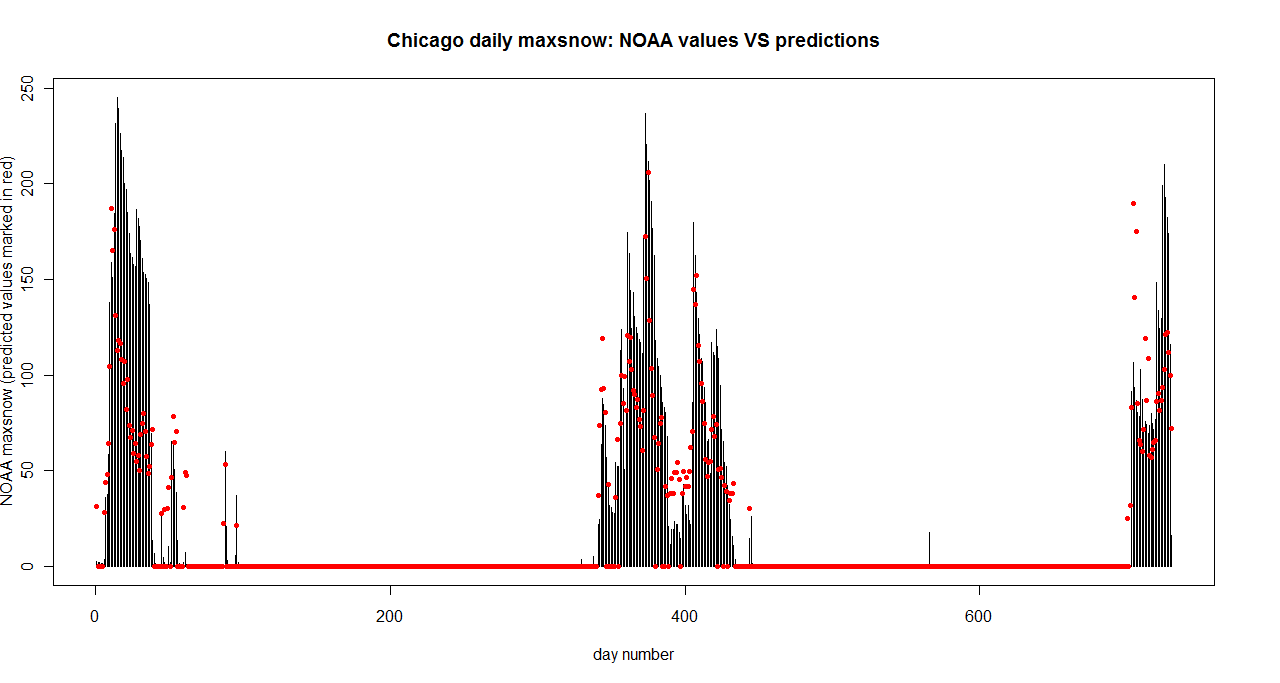
\includegraphics[width=0.5\textwidth,height=1.4in,clip,trim=0 0.5in 0in 0.6in]{plots/chicago_noaa_vs_prediction_prev_3.png} 
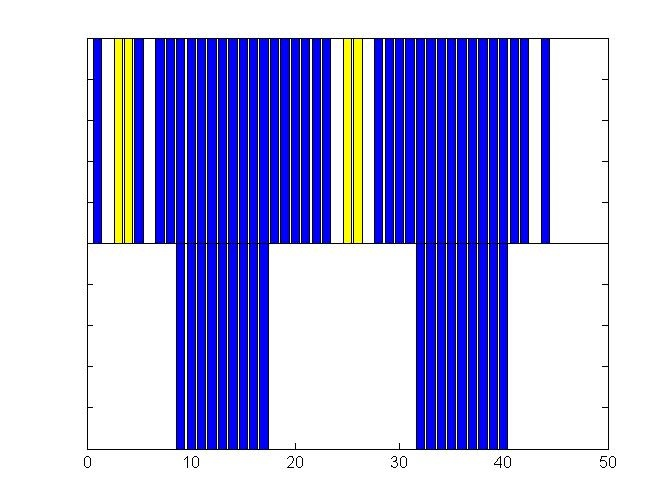
\includegraphics[width=0.14\textwidth]{bar/10816.jpg} \\
%(a) & (b)\\
\\
\end{tabular}
\end{center}
%}}
\vspace{-24pt}
\caption{Yellow bars show non-greenery at that time. Blue bars represent greenery. Prediction results on top shows 6 random places comparing to satellite ground truth. The ground truth on the bottom tends to disappear when leaves are turning yellow or green.}
\label{fig:placeinbar}
\vspace{-12pt}
\end{figure}

\subsubsection{Single time over places}

Sample maps are presented in figure ~\ref{fig:map}. These maps are visualizaton of the performance
in North America.
We use public sharing Flickr images.  
These images are more likely taken from more populated or more popular locations. The satellite ground truth, instead, is limited to cloud coverage and other sensor precision issue.


% (I should print an outline of continent as background of these maps.)

% bar plot of 2 places
\begin{figure}
%{\small{
\begin{center}
\begin{tabular}{cccc}
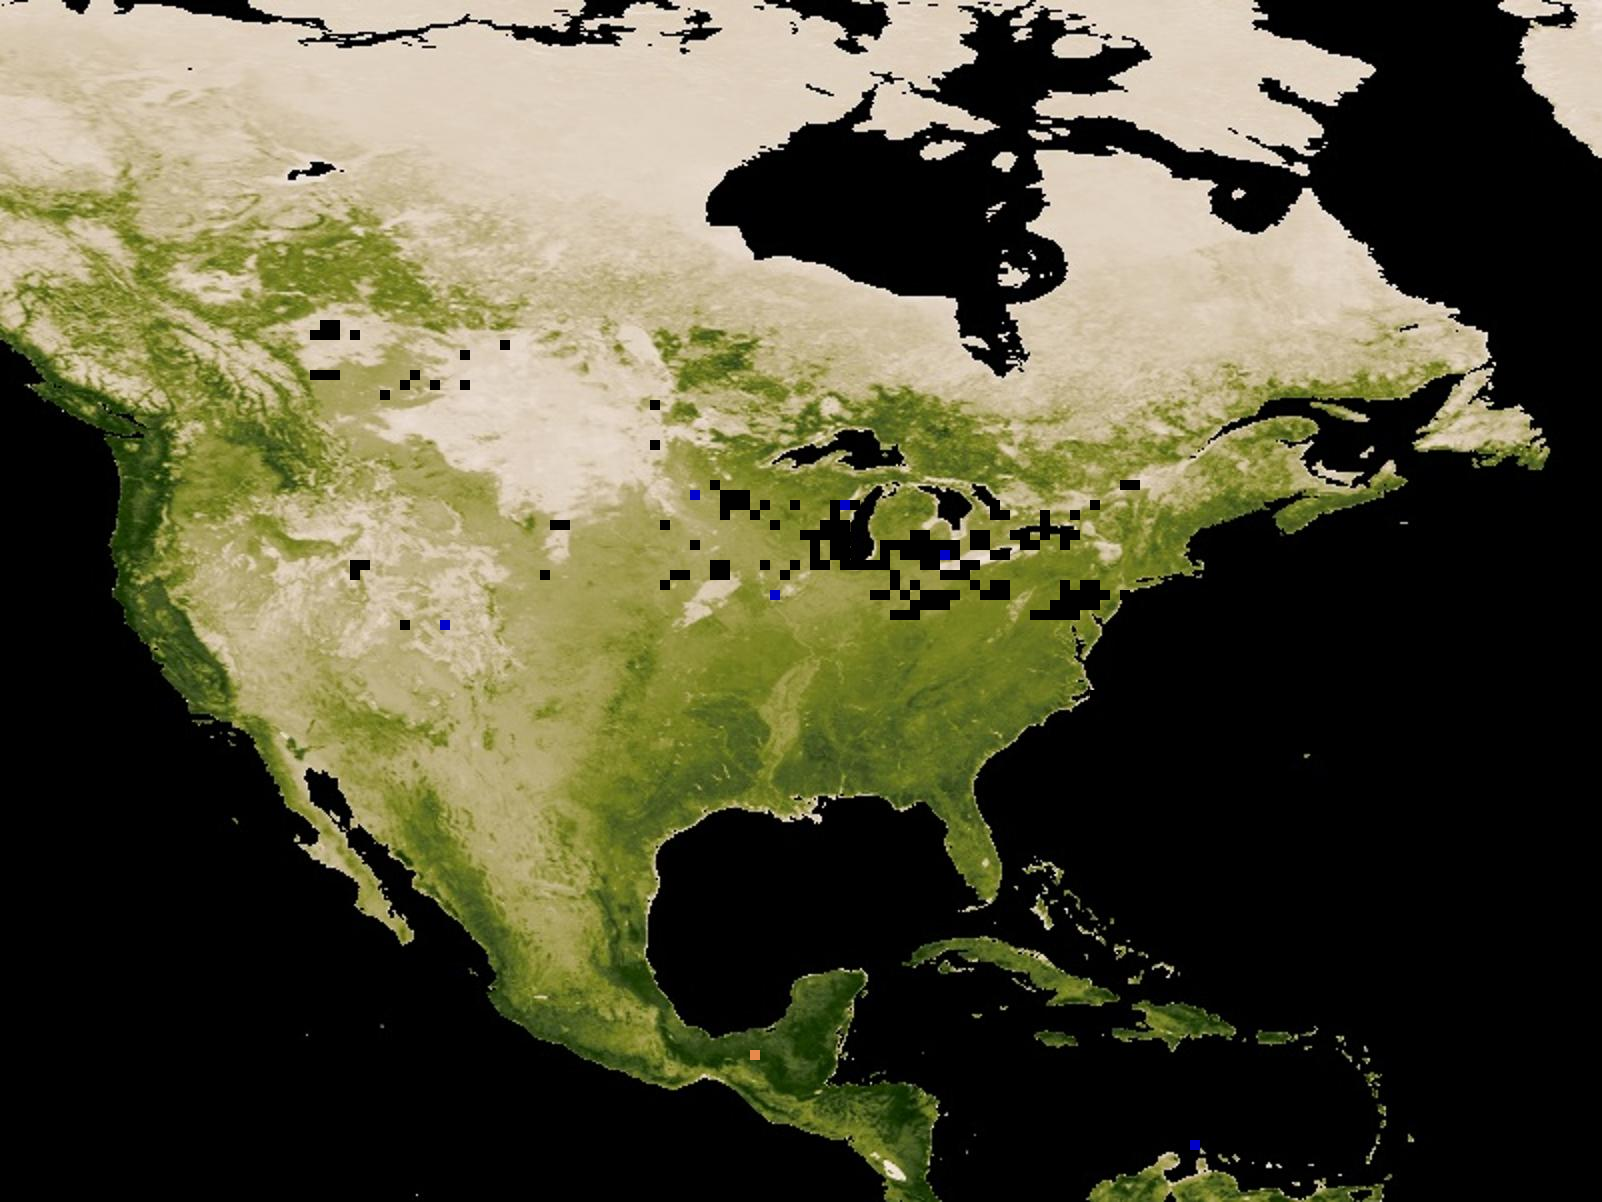
\includegraphics[width=0.10\textwidth]{map/72.png} &
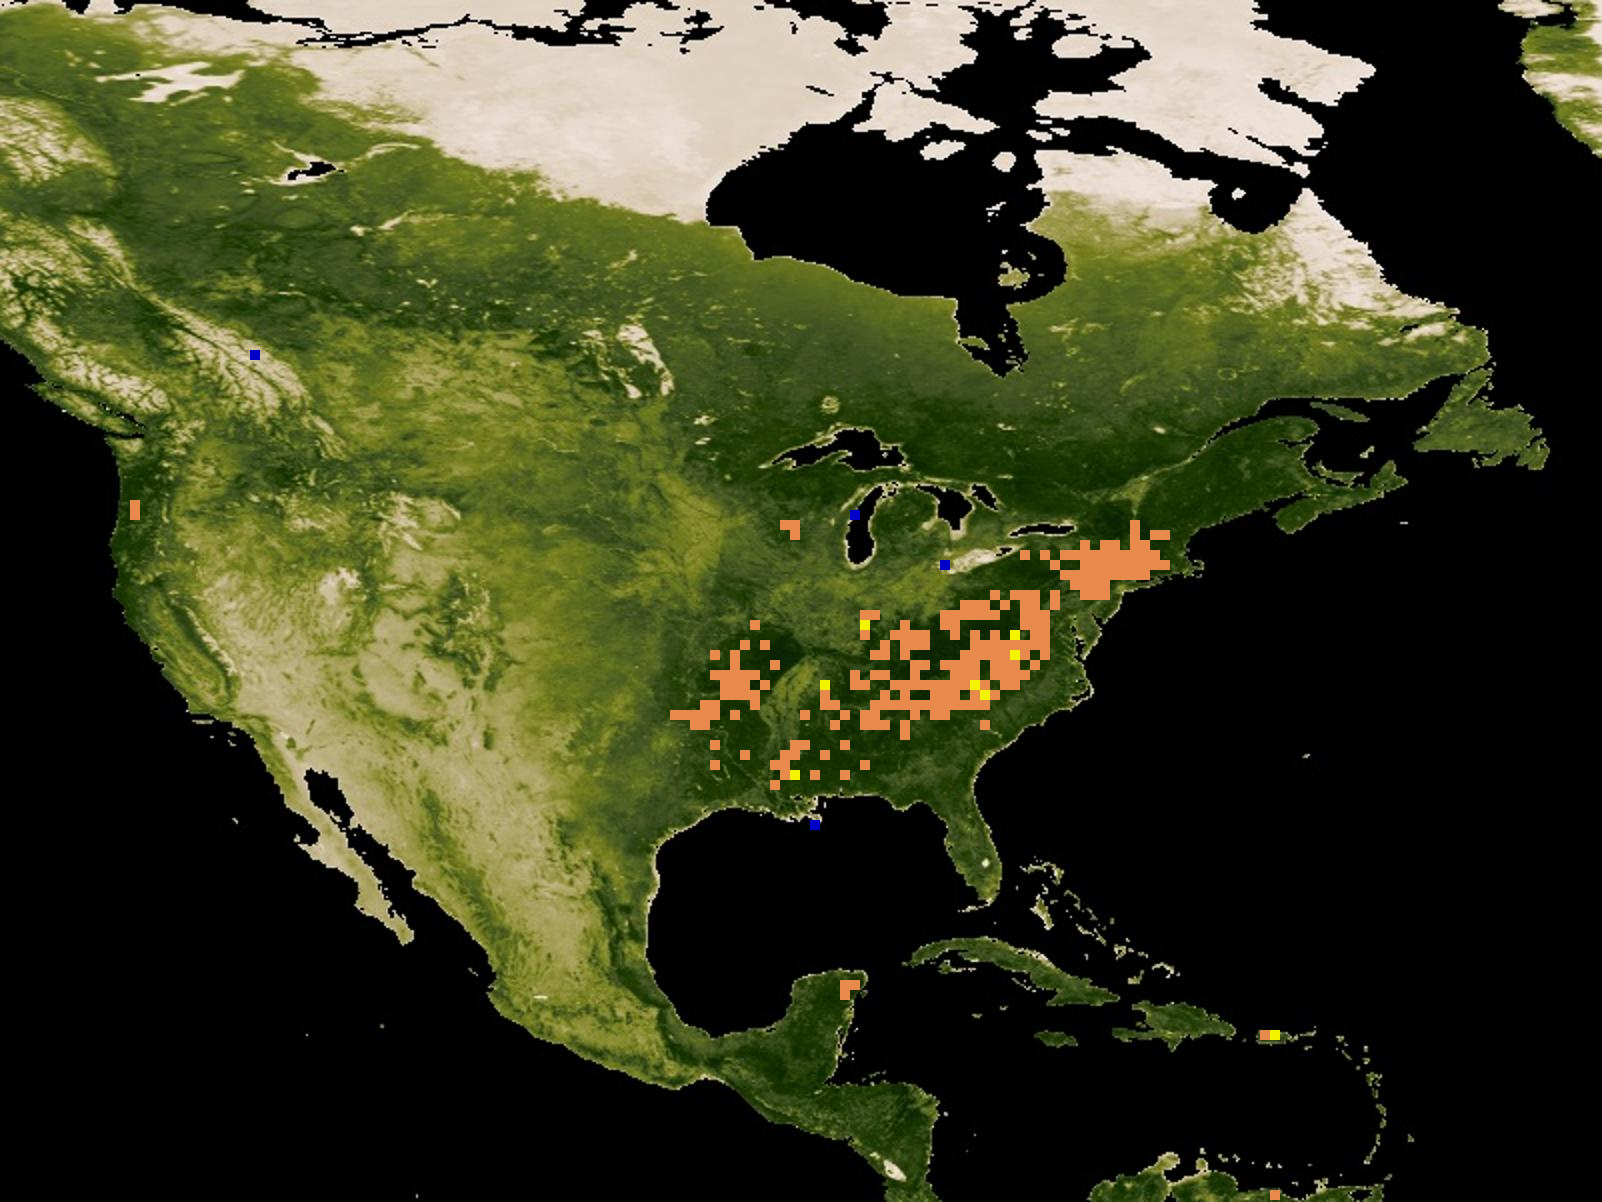
\includegraphics[width=0.10\textwidth]{map/77.png} &
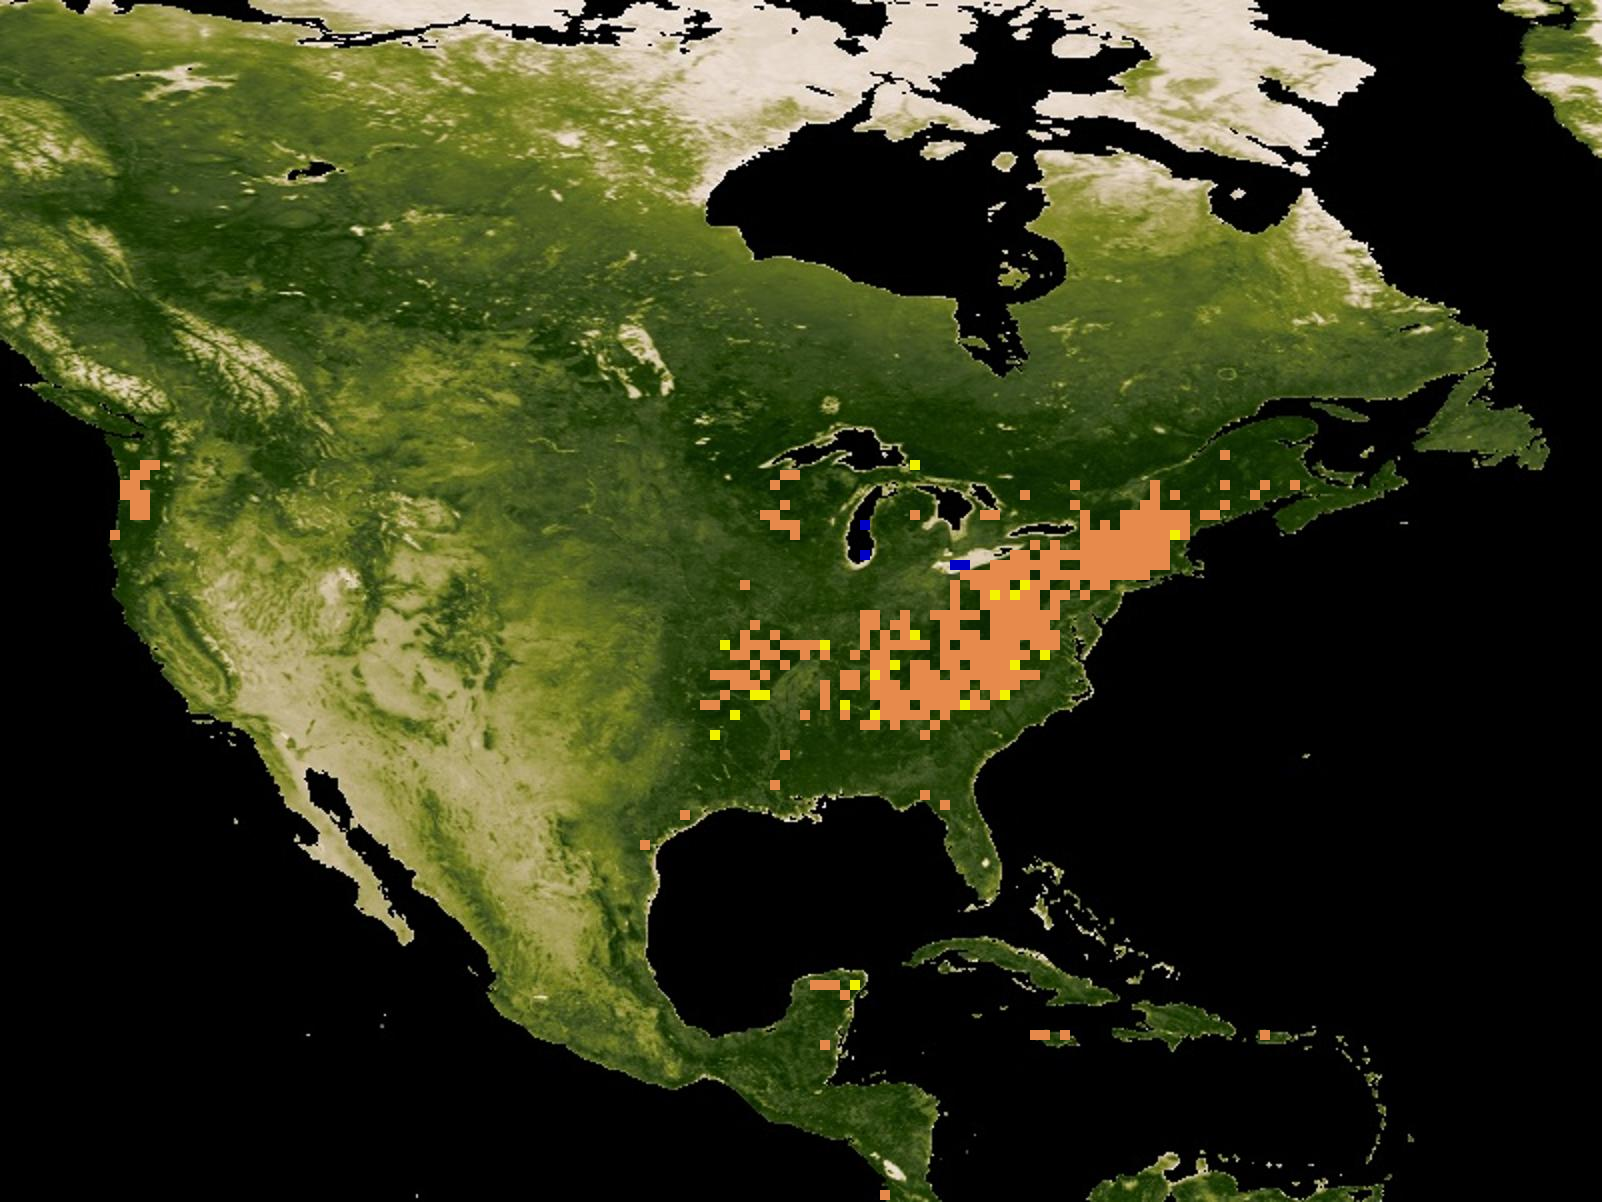
\includegraphics[width=0.10\textwidth]{map/78.png} &
%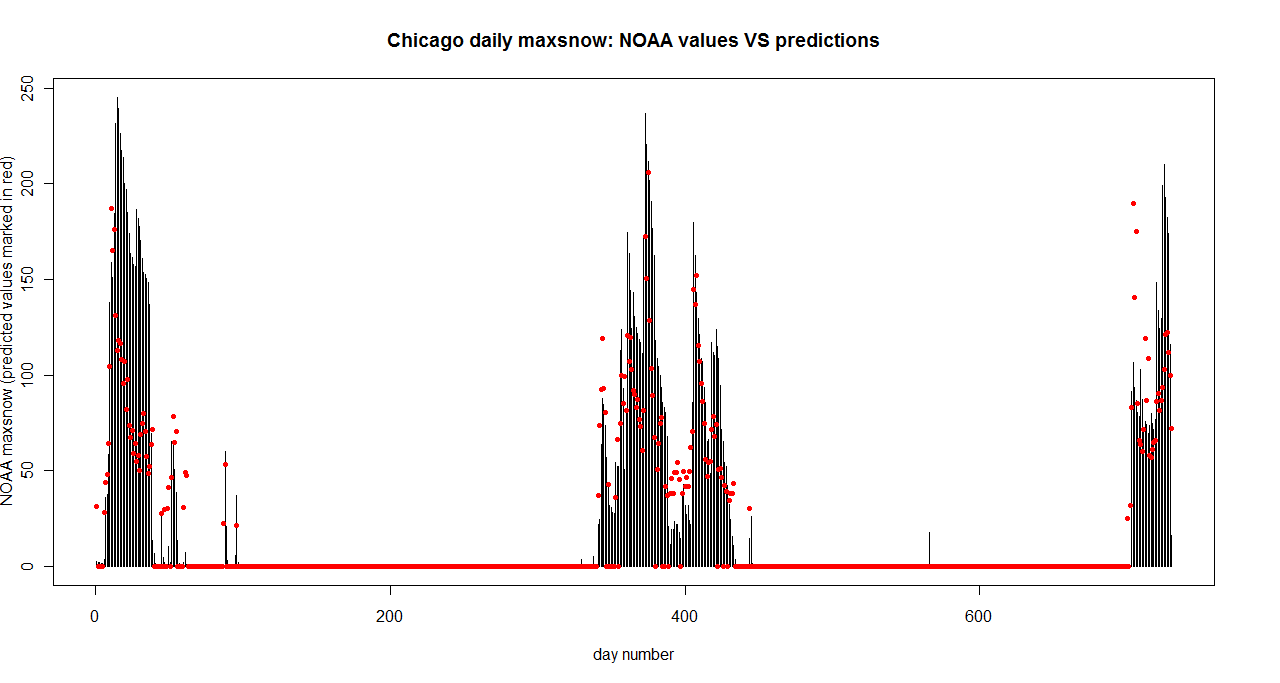
\includegraphics[width=0.5\textwidth,height=1.4in,clip,trim=0 0.5in 0in 0.6in]{plots/chicago_noaa_vs_prediction_prev_3.png} 
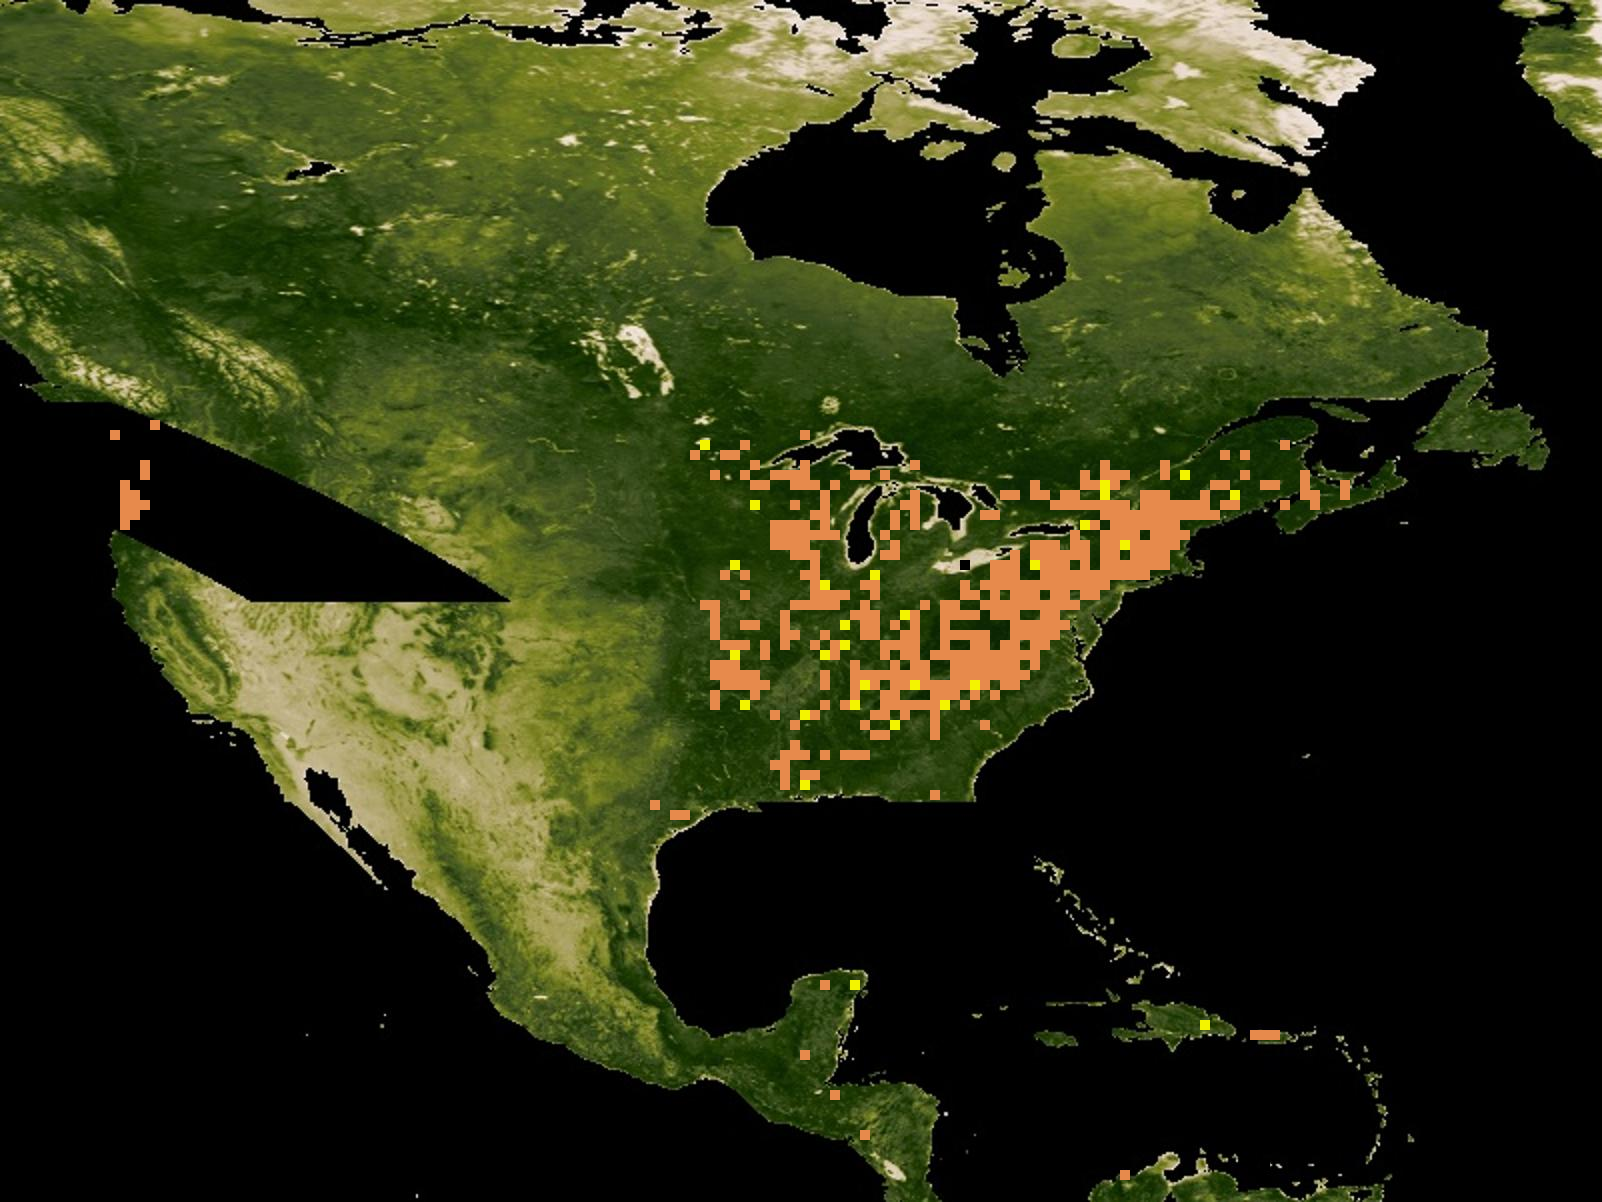
\includegraphics[width=0.10\textwidth]{map/79.png}  \\
Mar, 6th&May, 25th&Jun, 10th&Jun, 26th\\
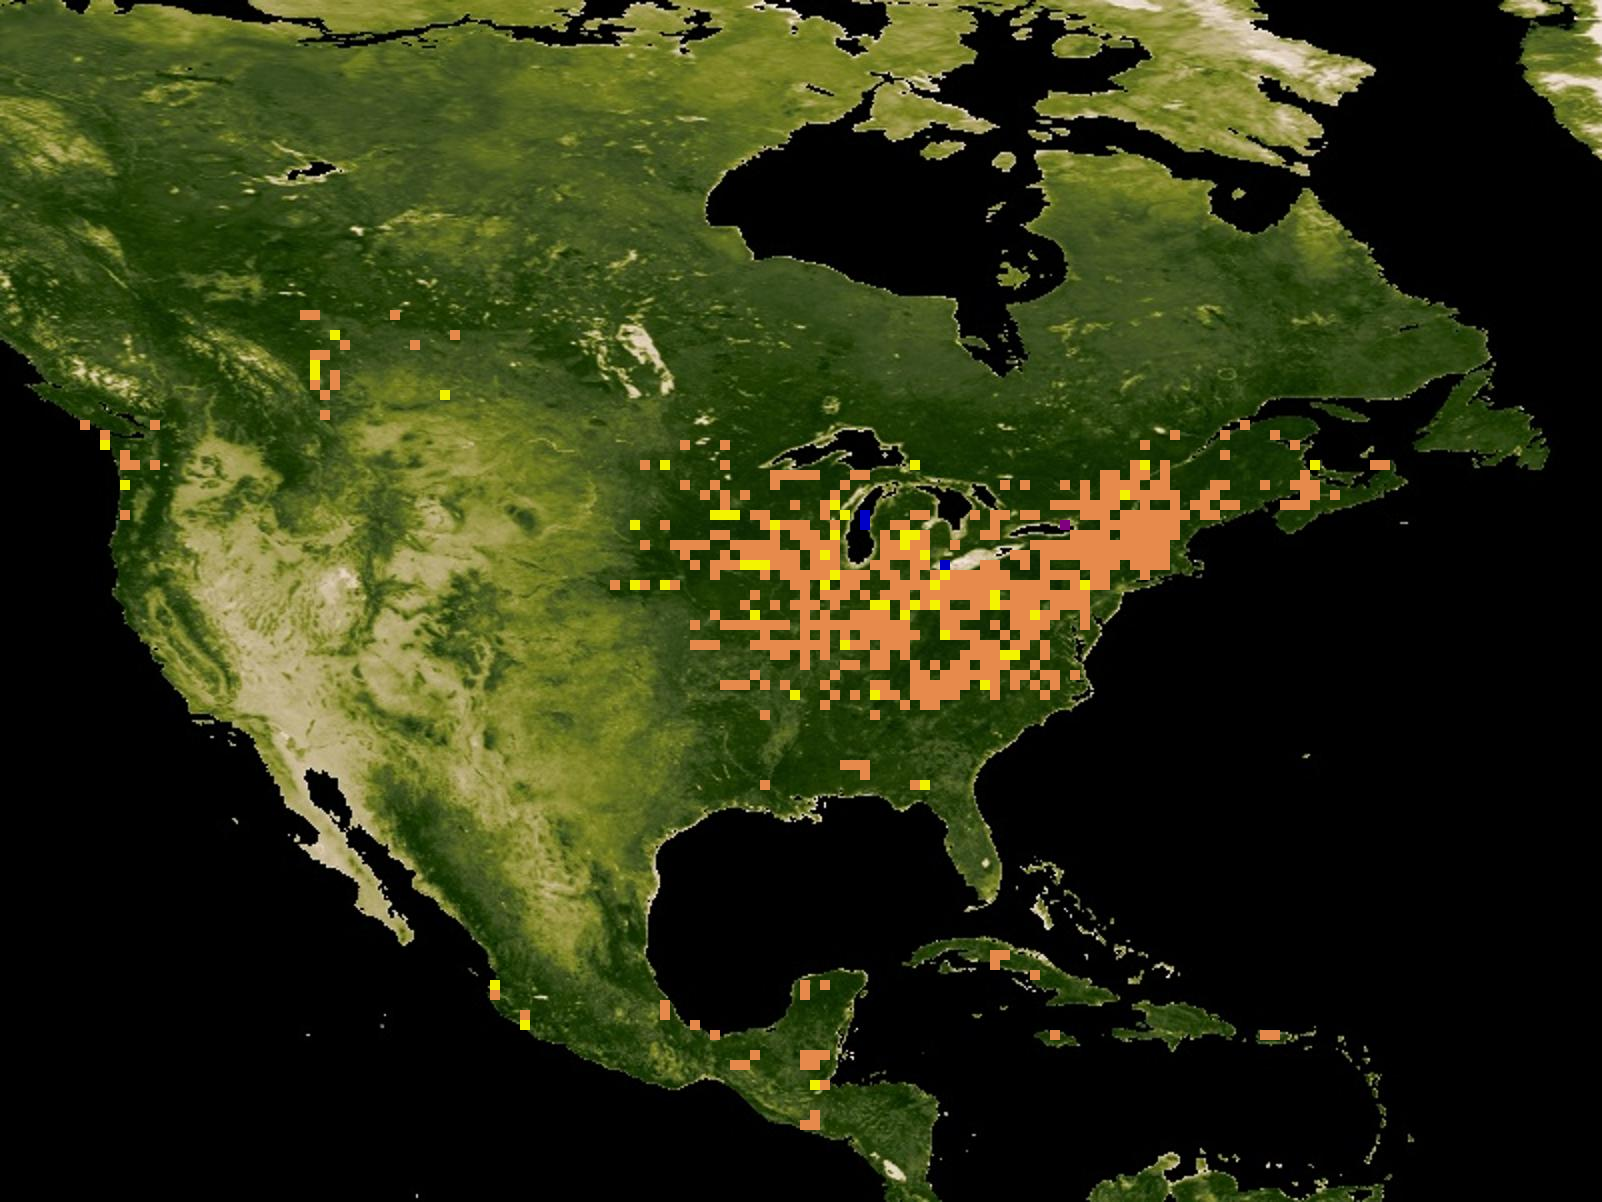
\includegraphics[width=0.10\textwidth]{map/82.png} &
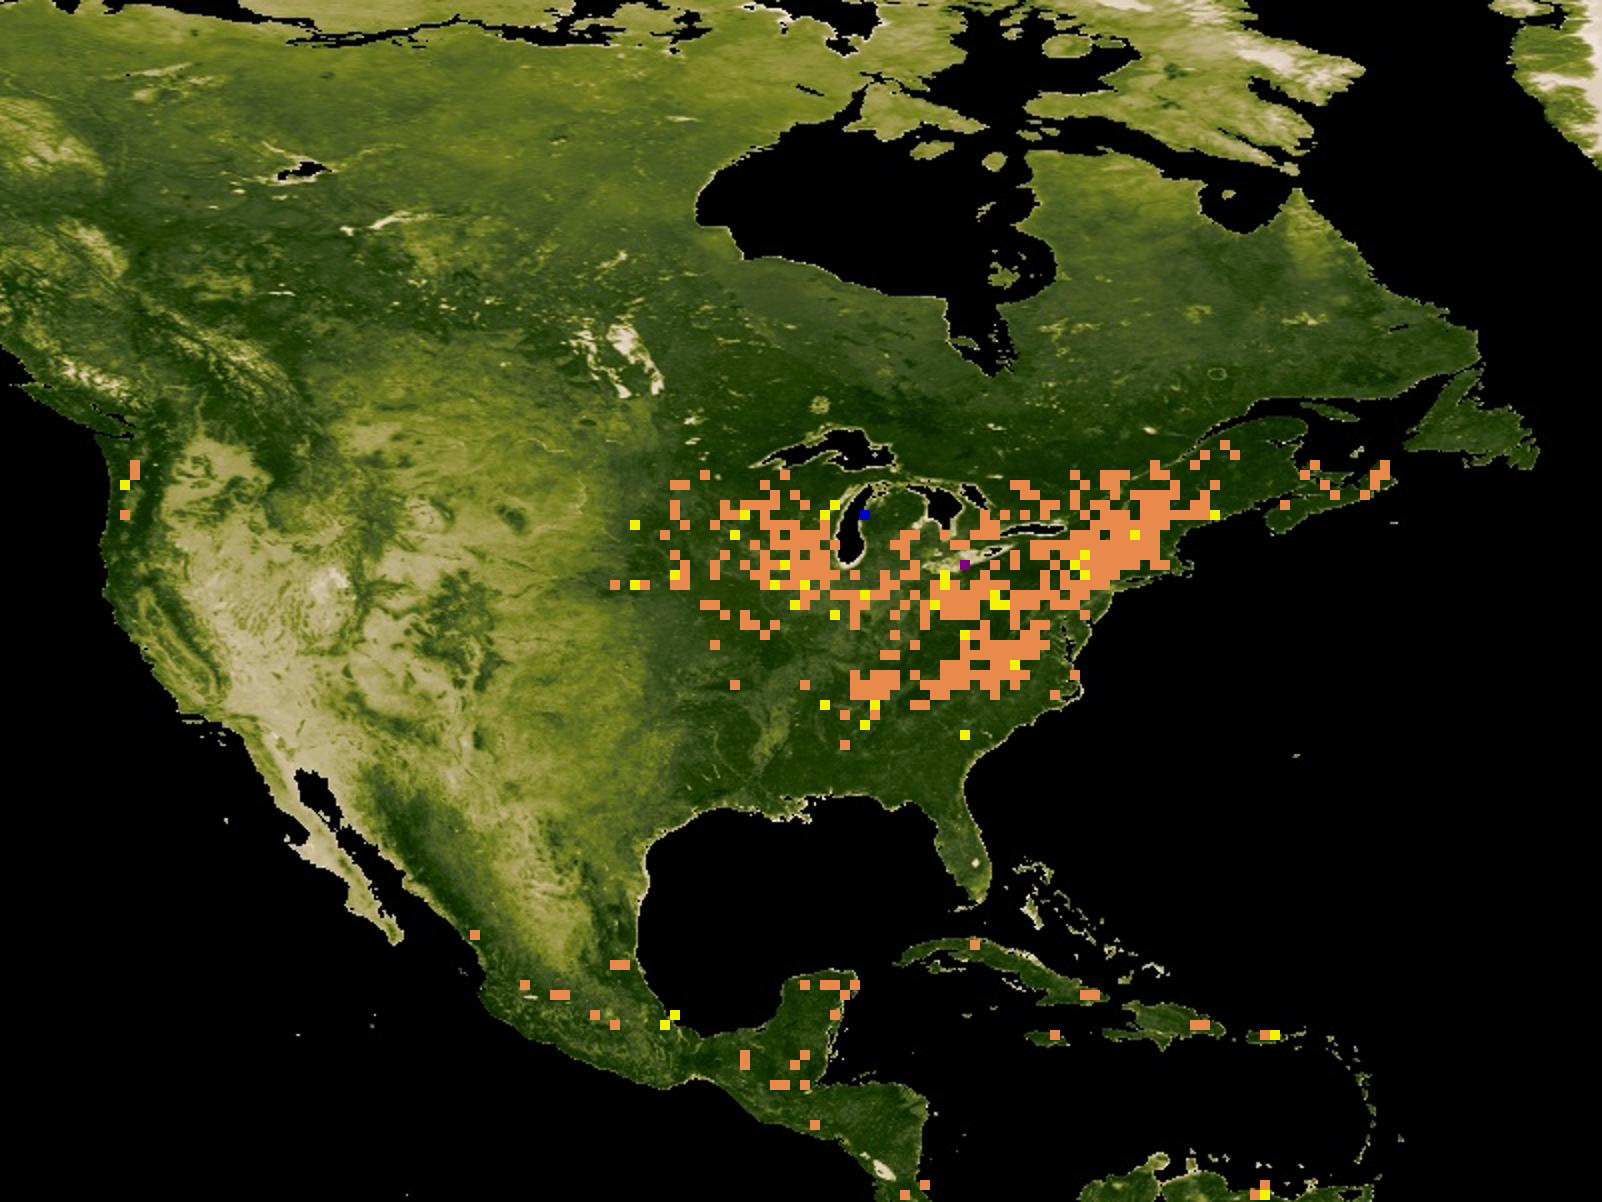
\includegraphics[width=0.10\textwidth]{map/83.png} &
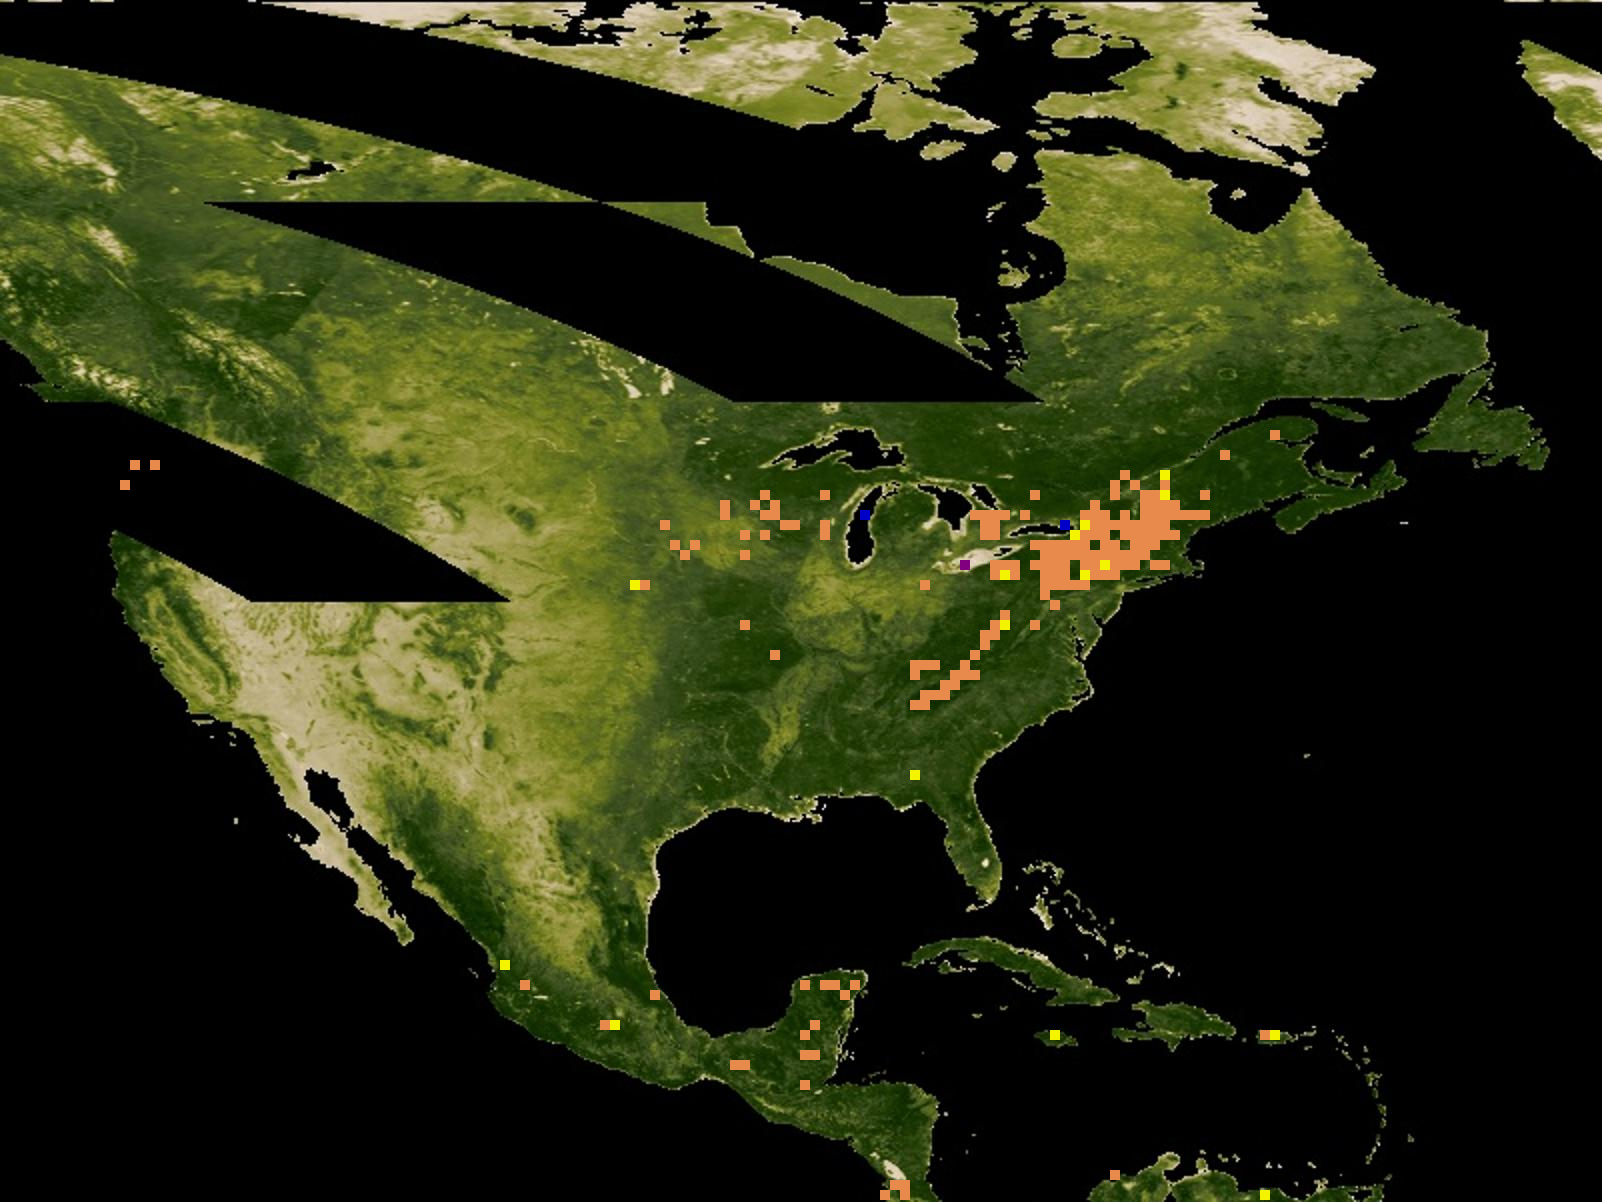
\includegraphics[width=0.10\textwidth]{map/84.png} &
%\includegraphics[width=0.5\textwidth,height=1.4in,clip,trim=0 0.5in 0in 0.6in]{plots/chicago_noaa_vs_prediction_prev_3.png} 
\includegraphics[width=0.10\textwidth]{map/91.png}  \\
Aug, 13th&Aug, 29th&Sep, 14th&Dec 19th\\
\\
\end{tabular}
\end{center}
%}}
\vspace{-24pt}
\caption{%On two 16-days time period, end of August on the left and during Christmas on the right, we show the confusion matrix map here. Orange bins are true positive; yellow bins are false negative; blue bins are false positive; and black bins are true negative.
We use prediction results to recreate vegetation coverage maps for each 16-days period. There are 8 maps picked in 2010. The dates under each map are the starting date of each 16-days period.
Orange bins represent true positive; blue bins are false positives; yellow bins are ture negatives and black bins are false negatives. }
\label{fig:map}
\vspace{-12pt}
\end{figure}
%
%\subsubsection{not using tag in vegetation case}
%
%We tested the performance of using only tags to make vegetation coverage prediction. The performance shows tag
%feature is not going to improve the result of using visual evidence.
%
%%%%%%%%%%%%    why this part     %%%%%%%%%%%%%%%%%
%%This is the result of vegetation case in www paper.
%%I guess this might help us to explain why we don't use tag in vege case in this paper.
%%%%%%%%%%%%%%%%%%%%%%%%%%%%%%%%%%%%%
%
%
%As shown in Figure~\ref{fig:greenery}, both curves outperform a random baseline for greenery prediction, but the estimates
%are not as accurate as those observed during in snow predictions. 
%% djc: conserving space...
%%For no greenery
%%predictions, when the threshold is 0, both combinations have
%%precisions above baselines. 50\% and 1\% threshold combination has
%%99.6\% for recall and 75.1\% for precision comparing to the 74.4\%
%%precision baseline, while 50\% and 5\% threshold combination has
%%99.6\% for recall and 84.6\% for precision comparing to the 84.2\%
%%precision baseline. However, the precisions drop when the absolute
%%values of the thresholds go up as shown in
%%Figure~\ref{fig:no_greenery}.  For the 50\% and 5\% threshold
%%combination, the curve is not smooth towards the left end as there are
%%very few predictions made which cause the precision to be unstable.
%%
%%
%There seem to be several reasons for this drop in performance.
%%The reason for this is yet to be explored. 
%One is that the boundary between greenery and no greenery
%seems more vague than the snow/no-snow boundary. 
%%Also, when it
%%snows people are more likely to tag with the term ``snow,''  comparing to tagging
%%"leaves" when leaves are green on a daily basis. For the 50\% and 1\%
%%threshold combination, p(greenery user|there is greenery) = 0.10 and
%%p(greenery user|there is no greenery) = 0.08, which is unlike that of
%%the snow data: when there is no snow, people seldom tag "snow".
%Moreover, the greenery ground truth data has a much coarser temporal resolution (16 days).
%Finally, it's less clear which tags should be used to estimate greenery; using color analysis of the visual content of images may be a better approach, which we leave for future work.
%%
%%
%%
%%#################################mk#################################################
%We also tried a learned classifier to predict greenery/non-greenery
%bins based on the set of tags used by all users in each bin and on
%each day.  We used the LibLinear classifier~\cite{Fan2008}
%because it performed well in case of snow classification. 
%Figure~\ref{fig:liblinear_greenery} presents the ROC curve for this classification task,
%showing an equal-error rate of about 91.6\%.
%%our data set for
%%vegetation classification task consists of 33611 exemplars, each of
%%which represents one bin in one day.  Of these samples only 3223
%%exemplars contains tags.  we evaluate the results by using 10 fold
%%cross validation and also by dividing the data into training set
%%contains exemplars from 2007 and 2008 years and testing set contains
%%exemplars from 2009 and 2010. table ~\ref{tab:classifier_greenerybins}
%%shows the results for both cases.
%
%\begin{figure}
%\begin{center}
%\begin{tabular}{cc}
%%%hp cr
%\includegraphics[width=0.35\textwidth]{plots/greenery.png}
%%%\includegraphics[width=0.35\textwidth,trim=1cm 0.5cm 1cm 1cm,clip]{plots/greenery.png}
%\end{tabular}
%\end{center}
%\vspace{-12pt}
%\caption{Greenery precision-recall curve using two different ground truth thresholds.}
%\label{fig:greenery}
%\end{figure}
%
%\begin{figure}
%\begin{center}
%\begin{tabular}{cc}
%\includegraphics[width=0.35\textwidth]{plots/greenery_LibLinear_Snow_1_curves_ROC.png}
%\end{tabular}
%\end{center}
%%%hp cr
%\vspace{-12pt}
%\caption{ROC curve for classifying greenery of bins, using tag features and LibLinear classifier.}
%\label{fig:liblinear_greenery}
%\end{figure}
%\vspace{-12pt}
%





%\subsection*{latest writing}
%\hfill \break
%\hfill \break
%
%\textbf{
%Two test cases: snow and vegetation. (Do we have any others?)
%}
%
%\textbf{
%For each of these, we learn visual (and maybe text) classifiers for individual images using our hand-labeled datasets. (Also the group datasets Dennis collected over summer?----?) We also learn parameters of the confidence score using satellite ground truth. (We don't learn visual models or text classifiers from the satellite ground truth.)}
%(---- Visual models  is not learnt from satellite but from hand-labeled images. Text classifier is learnt from satellite ground truth to determine snow/vege days or places.) 
%
%\textbf{We test }
%(---- vision model) 
%\textbf{on data collected after the training images.}                                             
%(---- Therefore, we get results of image prediction. And they are clustered according to location and time. 
%
%Then these images are used to compute confidence score of each place and time period.)
%\textbf{and we compare to satellite ground truth. For each of snow and vegetation, we present two kinds of results:}
%
%---- Overall numbers.
% (the numbers of overall prediction looks pretty good now. I put the results here and we can take it out any time we want)
%%% fp img grid to help explain every error
%
%\textbf{
%A. Single place over time: We choose a few places (cities or frequently-photographed places, maybe including a less-photographed place also for fairness) and look at their daily (biweekly for vegetation) estimate over 2-3 years. Plot these versus ground truth. Hopefully point out that the two track well -- i.e. that they spot time of leaf changes or major snow storms. Present quantitative results.
%}
%%% plot bars for all 13-14 overlaps
%
%\textbf{
%B. Single time over place: Choose a few days and show maps of our estimates versus ground truth on these days. Present quantitative results also.
%}
%%% cfmx 
%%% ask for just overlap prediction
%%% prepare a very complex: label on both side + cfmx
%
%\textbf{
%[I would of course be happiest if we also presented results over time and space, i.e. classifying every bin on every day. But the more I think about this, the more I'm not sure it's necessary... the quantitative results are hard to interpret anyway for all there reasons we've seen so far. I think if we did A and B well, we might not need to do this.]
%}( -- just a cool illustration or on top right of first page?)
%%% pic from /u/wang203/Desktop/spring12/ecology/wang203/snow/map2/img folder
%
%\hfill \break
%\hfill \break
%===================================
%\hfill \break
%\hfill \break

%\subsection{Test on vegetation cover}
%\subsubsection*{Vege hand labeled dataset}
%
%We build a data set with over 10000 images. They are taken before 2009, and are composed by images with "forest" and "summer" like tags and also random images without any tag preference. These images are labeled with categories 
%\textit{"Outdoor Greenery","Outdoor non-Greenery","Indoor","Other-modified"},and \textit{"Not available"}.
%
%Finally, we build a positive set with images in category \textit{"Outdoor Greenery"} and a negative set 
%with images in categories \textit{"Outdoor non-Greenery"} and \textit{"Indoor"}. To learn a image classification model, we build a training set with 4000 images and a testing set with 1900 images. In training and testing set, there are equal number of positive and negative samples.
%To show the diversity of our Flickr image dataset, in figure ~\ref{fig:dataset} we present a random sample of images in our vegetation dataset labeled as positive and negative.
%
%
%
%
%
%
%
%
%
%\begin{figure*}[th]
%{\small{
%\begin{center}
%\begin{tabular}{@{}c@{\,\,\,}c@{\,\,\,}c@{\,\,\,}c@{\,\,\,}c@{\,\,\,}}
%\includegraphics[width=0.19\textwidth]{imggrid/datasetposi/1.jpg} &
%\includegraphics[height=1in]{imggrid/datasetposi/2.jpg} &
%\includegraphics[width=0.19\textwidth]{imggrid/datasetposi/3.jpg} &
%\includegraphics[height=1in]{imggrid/datasetposi/4.jpg} &
%\includegraphics[width=0.19\textwidth]{imggrid/datasetposi/5.jpg} \\
%%\multicolumn{5}{c}{(a) Random positive images in vegetation dataset} \\
%\\[-6pt]
%\hline
%\\[-6pt]
%\includegraphics[height=1in]{imggrid/datasetposi/6.jpg} &
%\includegraphics[width=0.19\textwidth]{imggrid/datasetposi/7.jpg} &
%\includegraphics[width=0.19\textwidth]{imggrid/datasetposi/8.jpg} &
%\includegraphics[width=0.19\textwidth]{imggrid/datasetposi/9.jpg} &
%\includegraphics[width=0.19\textwidth]{imggrid/datasetposi/10.jpg} \\
%\multicolumn{5}{c}{(a) Random positive images in vegetation dataset} \\ 
%\\[-6pt]
%\hline
%\\[-6pt]
%\includegraphics[width=0.19\textwidth]{imggrid/datasetnega/1.jpg} &
%\includegraphics[width=0.19\textwidth]{imggrid/datasetnega/2.jpg} &
%\includegraphics[width=0.19\textwidth]{imggrid/datasetnega/3.jpg} &
%\includegraphics[width=0.19\textwidth]{imggrid/datasetnega/4.jpg} &
%\includegraphics[width=0.19\textwidth]{imggrid/datasetnega/5.jpg} \\
%%\multicolumn{5}{c}{(c) Random false negatives (snow images classified as non-snow)} \\ 
%\\[-6pt]
%\hline
%\\[-6pt]
%\includegraphics[height=1in]{imggrid/datasetnega/6.jpg} &
%\includegraphics[width=0.19\textwidth]{imggrid/datasetnega/7.jpg} &
%\includegraphics[width=0.19\textwidth]{imggrid/datasetnega/8.jpg} &
%\includegraphics[width=0.19\textwidth]{imggrid/datasetnega/9.jpg} &
%\includegraphics[width=0.19\textwidth]{imggrid/datasetnega/10.jpg} \\
%\multicolumn{5}{c}{(b) Random negative images in vegetation dataset} \\
%\end{tabular}
%\end{center}
%}}
%\caption{Random images from our hand-labeled dataset. Public sharing images are various in quality, contents, illumination and view angle.
%Negative images like winter trees without leaves, or indoor images capturing a photo of forest are more confusing.}
%\label{fig:dataset}
%\end{figure*}
%
%
%
%
%In vegetation detection, we use images on Flickr.com in year 2007 to 2010, with no tag limitation. We filter out the photos with inaccurate timestamps and geotags. We only use images with geotag precision no less than 13. (??? what's that mean?) 
%
%I paste this from David's email. The only thing is we use geotag precision >= 13 rather than 11. 
%
%[For geotags, there is an
%accuracy number right after the GPS coordinate in the merge\_files; we
%should ignore any photos with a number less than about 11. That means
%that the precision is less than about a city-scale. For timestamps,
%one thing that happens a lot is that people upload photos to Flickr
%that do not have timestamps -- e.g. scanned images. By default, Flickr
%gives this photo a timestamp of the day and time that it was
%*uploaded*. The first date in the merge\_files is the taken time and
%the second is the upload time. So if these two are the same, it means
%the taken time is probably not right and we should ignore the photo.
%Now one complication is that the two timestamps are in different time
%zones -- taken time is in the user's timezone while upload time is in
%Flickr's time zone (pacific time I think). So a simple rule is to
%simply remove any photos whose minutes and seconds are exactly the
%same for both taken time and upload time. That will unnecessarily
%remove about 1/(60*60)=1/3600 photos, but is a good simple rule.]
%
%


%\subsubsection*{Ground truth of vegetation -- NDVI index}
%%%%%%%% how much should the NDVI index value be mentioned?
%The ground truth is specified for every 16 days period. 
%And geometrically, north America area is divided into bins of 0.5 by 0.5 degree. This makes the north America area a 120*160 grid map.
%Only the days and bins with clear enough cloud coverage can be count as useful units. As in ~\cite{www paper}, a green bin must be covered by at least 50\% of green vegetation while a non-green bin only has less than 5\% of coverage.


% explain day bin, ground truth
%\subsubsection*{Vision model}
%Vegetation has the signature green color. The leaves of plants have distinctive visual texture. So we employ SIFT feature to analyze the local gradient distribution. And we also extract GIST feature to describe texture feature and global context. 
%
%
%
%
%
%\textbf{\textit{Color SIFT histogram.}}
%We extract dense SIFT feature on each of the RGB color plane, and concatenate them to build color SIFT feature. The dense SIFT feature is extracted from every 2 pixels by 2 pixels bin, with a step size of 5 pixels. In this way, we achieve representative key points and reasonable computation complex. 
%% Therefore we have 128*3-d for each key point
%% about 300-500 key points each images
%
%From training data set, We build 2000 dimensional centers of color SIFT feature using K-means clustering. With these centers, a 2000 dimensional histogram is built from all the key points of each image.
%
%Using SIFT histogram, a model is trained and tested with SVM using RBF kernel. 
%%Maybe the numbers should be in evaluation section        
%The performance is 78.10\%.
%
%\textbf{\textit{Color GIST.}}
%Similar to color SIFT feature, we also extract GIST feature from each of the RGB color plane.\\*\\*
%The performance is 82.58\%.
%
%\textbf{\textit{Combine visual features.}}
%The combined visual feature is built from concatenating the normalized GIST feature and SIFT histogram. A new model is learnt based on the combined feature.
%The performance is 85.9\%.
%
%\subsubsection*{Deep learning}
%(nothing special?)

%----------------------
%\subsection*{some may not necessary details for each test case}
%----------------------


%%%%%%%%%%%%%%%%

%\subsubsection*{Confidence score of vege}
%Confidence score is
%measuring the ratio of log likelihood of being a vegetation bin or not at each time period. All the prior statistics are learnt from satellite ground truth in 2007 and 2008.
%The prior probability is 24.8\% (I doubt this number. This is because the ground truth put too many bins in gray area while there are too many non-green bins on the north that we don't really care.) for a bin to be vegetation.
%For an image taken from a place covered by green vegetation at that time, the probability of this image being a green image is 27.18\%. On the other hand, it's only 3.03\% probability to see a green image in a place not covered by enough green vegetation at that time.
%
%
%
%\subsubsection*{Present vegetation detection results over space and time}
%
%We consider north America area has more images uploaded to photo-sharing website, and is also where Ecologists in the US would be interested in the changing color of vegetation. In our work, we define north America as latitude 10$^{\circ}$ to 70$^{\circ}$ and longitude -130$^{\circ}$ to -50$^{\circ}$.
%%\textdegree
%\hfill \break
%\hfill \break
%\xhdr{**Performance of vegetation detection in north America}
%\\*
%*** The performance using 2 threshold on confidence score with removing bad timestamps\\*
%\\*
%on + day and bin, the probability of an img is +, p(s|+) = 0.271778644215\\*
%on - day and bin, the probability of an img is +, p(s|-) = 0.0303125\\*
%\\*
%num of bins gt shows nongreen = 32657\\*
%overlap of gt and predi both shows nongreen = 400\\*
%accuracy = 0.012248522522\\*
%num of bins predi shows green = 16545\\*
%overlap of gt and predi both shows green = 2580\\*
%accuracy = 0.155938349955\\*
%num of bins that both have data = 3369\\*
%overlap = 2980\\*
%accuracy = 0.884535470466\\*
%num of bins that predi have data = 25950\\*
%num of bins that gt have data = 43446\\*
%ratio = 0.597293191548\\*
%in bins both have data, num of predi as gr = 2616\\*
%overlap = 2580\\*
%precision of gr = 0.98623853211\\*
%in bins both have data, num of predi as nongr = 753\\*
%overlap = 400\\*
%precision of nongr = 0.531208499336\\*
%in bins both have data, num of gt as gr = 2933\\*
%overlap = 2580\\*
%recall of gr = 0.879645414252\\*
%in bins both have data, num of gt as nongr = 436\\*
%overlap = 400\\*
%recall of nongr = 0.917431192661\\*
%
%The random baseline from ground truth is\\*
%2933+436\\*
%3369\\*
%2933/3369\\*
%.87058474324725437815\\*
%\\*
%***confusion matrix maps and data
%
%\begin{table}[b]
%\begin{center}
%{\footnotesize{
%\begin{tabular}{|l|c|c|}
%\hline 
%--- & \multicolumn{2}{c|}{Ground truth}\tabularnewline
%\hline
%--- & Greenery & Non-Greenery\tabularnewline
%\hline 
%\hline 
%%Random Baseline  & --- & 50.0\%\tabularnewline
%%\hline 
%%\hline
%Greenery & 2580 & 36\tabularnewline
%\hline 
%Non-Greenery & 353 & 400\tabularnewline
%\hline
%\end{tabular}
%}}
%\caption{Confusion matrix of vegetation detection in 2007}
%\label{tab:confusionmatrix}
%\end{center}
%\end{table}
%(This table looks terrible. Hope there is a way to make it prettier.)
%(??? Result is presented in video. Is a map necessary here? or a better way?)
%\\*
%***explain errors
%
%\begin{figure*}[th]
%{\small{
%\begin{center}
%\begin{tabular}{@{}c@{\,\,\,}c@{\,\,\,}c@{\,\,\,}c@{\,\,\,}c@{\,\,\,}}
%\includegraphics[width=0.19\textwidth]{imggrid/falseposi/1.jpg} &
%\includegraphics[width=0.19\textwidth]{imggrid/falseposi/2.jpg} &
%\includegraphics[height=1in]{imggrid/falseposi/3.jpg} &
%\includegraphics[height=1in]{imggrid/falseposi/4.jpg} &
%\includegraphics[height=1in]{imggrid/falseposi/5.jpg} \\
%%\multicolumn{5}{c}{(a) Random positive images in vegetation dataset} \\
%\\[-6pt]
%\hline
%\\[-6pt]
%\includegraphics[width=0.19\textwidth]{imggrid/falseposi/6.jpg} &
%\includegraphics[width=0.19\textwidth]{imggrid/falseposi/7.jpg} &
%\includegraphics[width=0.19\textwidth]{imggrid/falseposi/8.jpg} &
%\includegraphics[width=0.19\textwidth]{imggrid/falseposi/9.jpg} &
%\includegraphics[width=0.19\textwidth]{imggrid/falseposi/10.jpg} \\
%%\multicolumn{5}{c}{(a) Random positive images in vegetation dataset} \\ 
%\\[-6pt]
%\hline
%\\[-6pt]
%\includegraphics[height=1in]{imggrid/falseposi/11.jpg} &
%\includegraphics[height=1in]{imggrid/falseposi/12.jpg} &
%\includegraphics[width=0.19\textwidth]{imggrid/falseposi/13.jpg} &
%\includegraphics[width=0.19\textwidth]{imggrid/falseposi/14.jpg} &
%\includegraphics[height=1in]{imggrid/falseposi/15.jpg} \\
%%\multicolumn{5}{c}{(c) Random false negatives (snow images classified as non-snow)} \\ 
%\\[-6pt]
%\hline
%\\[-6pt]
%\includegraphics[width=0.19\textwidth]{imggrid/falseposi/16.jpg} &
%\includegraphics[width=0.19\textwidth]{imggrid/falseposi/17.jpg} &
%\includegraphics[width=0.19\textwidth]{imggrid/falseposi/18.jpg} &
%\includegraphics[height=1in]{imggrid/falseposi/19.jpg} &
%\includegraphics[width=0.19\textwidth]{imggrid/falseposi/20.jpg} \\
%%\multicolumn{5}{c}{(b) Random negative images in vegetation dataset} \\
%\end{tabular}
%\end{center}
%}}
%\caption{In all false positive bins, there are 47 images that are predicted as greenery. And these images are the reason these bins are predicted as green. Here are some random selected examples of the green images.}
%\label{fig:falseposi}
%\end{figure*}
%Generally, all the false negative error is due to the sparseness of data. While not enough images are collected at certain location during some time, there is either no green image found or green images are too few compare to the quantity of non-green images. On the other hand, false positive error is rare (less than 1\%) and complex. We found most images in the false positive bins are actually green vegetation images. ( here we need some more explanation) In figure ~\ref{fig:falseposi}, we show some examples of images in false positive bins.
%
%
%
%\begin{figure*}[th]
%{\small{
%\begin{center}
%\begin{tabular}{@{}c@{\,\,\,}c@{\,\,\,}c@{\,\,\,}c@{\,\,\,}c@{\,\,\,}}
%\includegraphics[width=0.19\textwidth]{imggrid/falseposi/1.jpg} &
%\includegraphics[width=0.19\textwidth]{imggrid/falseposi/2.jpg} &
%\includegraphics[height=1in]{imggrid/falseposi/3.jpg} &
%\includegraphics[height=1in]{imggrid/falseposi/4.jpg} &
%\includegraphics[height=1in]{imggrid/falseposi/5.jpg} \\
%%\multicolumn{5}{c}{(a) Random positive images in vegetation dataset} \\
%\\[-6pt]
%\hline
%\\[-6pt]
%\includegraphics[width=0.19\textwidth]{imggrid/falseposi/6.jpg} &
%\includegraphics[width=0.19\textwidth]{imggrid/falseposi/7.jpg} &
%\includegraphics[width=0.19\textwidth]{imggrid/falseposi/8.jpg} &
%\includegraphics[width=0.19\textwidth]{imggrid/falseposi/9.jpg} &
%\includegraphics[width=0.19\textwidth]{imggrid/falseposi/10.jpg} \\
%\multicolumn{5}{c}{(a) Random positive images in vegetation dataset} \\ 
%\\[-6pt]
%\hline
%\\[-6pt]
%\includegraphics[height=1in]{imggrid/falseposi/11.jpg} &
%\includegraphics[height=1in]{imggrid/falseposi/12.jpg} &
%\includegraphics[width=0.19\textwidth]{imggrid/falseposi/13.jpg} &
%\includegraphics[width=0.19\textwidth]{imggrid/falseposi/14.jpg} &
%\includegraphics[height=1in]{imggrid/falseposi/15.jpg} \\
%%\multicolumn{5}{c}{(c) Random false negatives (snow images classified as non-snow)} \\ 
%\\[-6pt]
%\hline
%\\[-6pt]
%\includegraphics[width=0.19\textwidth]{imggrid/falseposi/16.jpg} &
%\includegraphics[width=0.19\textwidth]{imggrid/falseposi/17.jpg} &
%\includegraphics[width=0.19\textwidth]{imggrid/falseposi/18.jpg} &
%\includegraphics[height=1in]{imggrid/falseposi/19.jpg} &
%\includegraphics[width=0.19\textwidth]{imggrid/falseposi/20.jpg} \\
%\multicolumn{5}{c}{(b) Random negative images in vegetation dataset} \\
%\end{tabular}
%\end{center}
%}}
%\caption{In all false positive bins, there are 47 images that are predicted as greenery. And these images are the reason these bins are predicted as green. Here are some random selected examples of the green images.}
%\label{fig:falseposi}
%\end{figure*}
%
%
%\xhdr{**Single place over time}
%
%figure ~\ref{fig:placeinbar} 
%
%% bar plot of 2 places
%\begin{figure}
%%{\small{
%\begin{center}
%\begin{tabular}{c c}
%\includegraphics[width=0.22\textwidth]{bar1.jpg} &
%%\includegraphics[width=0.5\textwidth,height=1.4in,clip,trim=0 0.5in 0in 0.6in]{plots/chicago_noaa_vs_prediction_prev_3.png} 
%\includegraphics[width=0.22\textwidth]{bar2.jpg} \\
%(a) & (b)\\
%\\
%\end{tabular}
%\end{center}
%%}}
%\vspace{-24pt}
%\caption{Yellow bars show non-greenery at that time. Blue bars represent greenery. Prediction results on top shows 2 random places comparing to satellite ground truth. The ground truth on the bottom tends to disappear when leaves are turning yellow or green.}
%\label{fig:placeinbar}
%\vspace{-12pt}
%\end{figure}
%
%\xhdr{**Single time over place}
%
%Sample maps are presented in figure ~\ref{fig:map}. (I should print an outline of continent as background of these maps.)
%
%% bar plot of 2 places
%\begin{figure}
%%{\small{
%\begin{center}
%\begin{tabular}{c c}
%\includegraphics[width=0.22\textwidth]{imggrid/13.png} &
%%\includegraphics[width=0.5\textwidth,height=1.4in,clip,trim=0 0.5in 0in 0.6in]{plots/chicago_noaa_vs_prediction_prev_3.png} 
%\includegraphics[width=0.22\textwidth]{imggrid/22.png} \\
%(a) & (b)\\
%\\
%\end{tabular}
%\end{center}
%%}}
%\vspace{-24pt}
%\caption{On two 16-days time period, end of August on the left and during Christmas on the right, we show the confusion matrix map here. Orange bins are true positive; yellow bins are false negative; blue bins are false positive; and black bins are true negative.}
%\label{fig:map}
%\vspace{-12pt}
%\end{figure}
%
%\hfill \break
%\hfill \break
%===================================
%\hfill \break
%\hfill \break
%\subsection*{workshop}
%\subsection{Snow detection}
%
%
%As noted above, we are aware of very little work that has considered
%the problem of detecting snow in images: the most relevant
%work~\cite{singhal2003spatialcontext} considers snow in the context of
%natural materials classification, but is over 10 years old, uses a
%small and biased dataset, and does not report classification results.
%Recent work on scene understanding~\cite{XiaoHEOT10} sometimes
%includes snow-related scenes, but none of this work applies directly
%to our problem because snow can appear across a range of different
%scene types. Snow is really an object, not a type of scene, but we are
%not aware of any work on recognizing snow in the object detection
%literature.
%
%We thus begin by assembling a large-scale realistic image dataset,
%and test a variety of modern classification techniques on the
%problem of snowy scene detection. We use a labeled subset of this
%dataset to train classifiers and to test their performance, and then
%apply these classifiers to the problem of generating satellite-like
%snowfall maps using image analysis on geo-tagged, time-stamped
%Flickr photos.
%
%\input{dataset}
%\input{snowclassification}
%\input{flowerclassification}
%%\subsection{Classifiers}
%
%%We trained different SVM classifiers using different kernels ...........
%
%\hfill \break
%\hfill \break
%===================================
%\hfill \break
%\hfill \break
%\subsection{www -- snow coverage}
%
%\label{sec:results}
%
%We now turn to presenting experimental results for estimating the
%geo-temporal distributions of two ecological phenomena: snow and vegetation cover.
%In addition to the likelihood ratio-based score described in
%Section~\ref{sec:results} and machine learning approaches, we also
%compare to two simpler techniques: \textit{voting,} in which 
%we simply count the number of users that use one of a set
%$S$ of tags related to the phenomenon of interest at a given time and place, and
%\textit{percentage,} in which we calculate the ratio of users that use
%one of the tags in $S$ over the total number of users who took a photo
%in that place on that day.
%
%\subsubsection*{Snow prediction in cities}
%
%%%%%%%%%%%%%%%%%%%%%%%
%% hz added this for ROC curves
%% We convert this problem to a binary prediction problem to compare different method with ROC curves. For each method, we slide a threshold for the bins that have photos. Predictions will be made only for the bins with ground truth and photos for which snow bins are positive cases and non-snow bins are negative cases.
%% The confidence method and percentage method have single values to threshold while for voting method, we split it into two, as it has snow voters and no-snow voters. To make predictions using number of no-snow voters, we require the number of snow voters to be zero, while we don't consider the number of no-snow voters when using snow voters as thresholding values to make predictions. The baseline TPR for confidence, percentage and snow-voter voting is 2.76\%. % or 97.24%?
%% and the baseline TPR for no-snow voter is 1.90\% (is it useful to use no-snow voter number to predict snow?)
%
%% baseline_positive/baseline_total:0.0275996280425
%
%% We first consider 
%
%% \section{NOAA dataset}
%
%
%We first test how well the Flickr data can predict snowfall at a local
%level, and in particular for cities in which high-quality
%surface-based snowfall observations exist and for which photo density is high.
%%
%%% We want to use it as a complete and reliable ground truth of daily
%%% snow presence for major US cities where the Flickr user population is
%%% also dense, such that we are able to train and test on the NOAA and
%%% Flickr dataset to predict snow presence and even quantify it for every
%%% day.
%%
%We choose 4 U.S. metropolitan areas, New York City, Boston, Chicago and
%Philadelphia, and try to predict both daily snow presence as well as
%the quantity of snowfall.  For each city, we define a corresponding
%geospatial bounding box and select the NOAA ground observation stations in that area. 
%For example, 
%Figure~\ref{tab:city_statistics} shows the the stations 
%and the bounding box for 
%New York City. We calculate the ground truth daily snow quantity for a city as the average of
%the valid 
%snowfall values from its stations.
%%, with the
%%daily snow depth value obtained in a similar way. 
%%% According to the
%%% Climatological Data Publications
%%% (http://www7.ncdc.noaa.gov/IPS/cd/cd.html) that are generated from
%%% GHCN-Daily, the snowfall values reflect snowfall from 0 to 24 local
%%% time daily in millimeters while the snow depth values are recorded
%%% once at 12 UTC (GMT). So the snowfall after 12 UTC (GMT) that day is
%%% not reflected by the snow depth value for that day. So we decide to
%%% take the max value between the snowfall value and snow depth value as
%%% an estimation of the quantity of snow presence on a particular day and
%%% we call this value max\_snow.
%We call any day with a non-zero snowfall or snowcover to be a snow day,
%and any other day to be a non-snow day.
%%and make binary snow presence predictions, we need to define ground
%truth snow and non-snow days: we let  days with max\_snow greater than 0
%be snow days and the rest be non-snow
%days. 
%Figure~\ref{tab:city_statistics} also presents some basic statistics for
%these 4 cities.  All of our experiments involve 4 years (1461 days) of
%data from January 2007 through December 2010; we reserve the first two
%years for training and validation, and the second two years for
%testing.
%
%%<<<<<<< .mine
%%=======
%%We choose 4 major cities in the US - New York City, Boston, Chicago
%%and Philadelphia to predict their daily snow presence and the quantity
%%of snow presence.  For each city, we choose a corresponding geo area
%%and a list of reliable stations in that area defined and chosen by the
%%Climatological Data Publications. In fig
%%Figure~\ref{fig:nyc_stations}, we mark the stations we collect data
%%from and the bounding box for selecting geostamped Flickr photos for
%%New York City. The daily snowfall for a certain city is the average of
%%the valid snowfall values from the stations in the defined area. The
%%daily snow depth value is obtained in a similar way. 
%
%%% According to the
%%% Climatological Data Publications
%%% ~\cite{noaa2} %(http://www7.ncdc.noaa.gov/IPS/cd/cd.html) that are
%%% generated from GHCN-Daily, the snowfall values reflect snowfall from 0
%%% to 24 local time daily in millimeters while the snow depth values are
%%% recorded once at 12 UTC (GMT). So the snowfall after 12 UTC (GMT) that
%%% day is not reflected by the snow depth value for that day. So we
%%% decide to take the max value between the snowfall value and snow depth
%%% value as an estimation of the quantity of snow presence on a
%%% particular day and we call this value max\_snow.  In order to compute
%%% Flickr confidence and make binary snow presence predictions, we need
%%% to define ground truth snow and non-snow days. The days with max\_snow
%%% greater than 0 are snow days and the days with max\_snow equal to 0
%%% are non-snow days. Table~\ref{tab:city_statistics} shows some basic
%%% statistics of the 4 cities.
%
%
%\begin{figure}
%\begin{center}
%%\begin{tabular}{c}
%\includegraphics[width=0.35\textwidth]{plots/nyc_stations.png} 
%%\end{tabular}
%\end{center}
%%\caption{New York City geospatial bounding box used to select Flickr photos, and locations of NOAA observation stations.}
%%\label{fig:nyc_stations}
%%\end{figure}
%%
%%
%%
%%\begin{table} 
%% \caption {\textbf{Statistics about spatial area, photo density, and ground truth for each of the 4 cities.}}
%%\label{tab:city_statistics} 
%\begin{center}
%{\small{
%\newcommand{\spc}{\hspace{2pt}}
%\begin{tabular} {|@{\spc}l@{\spc}|@{\spc}r@{\spc}|@{\spc}r@{\spc}|@{\spc}r@{\spc}|@{\spc}r@{\spc}|} 
%\hline 
%\textbf{} &{NYC}  &{Chicago} &{Boston}&{Philadelphia} \tabularnewline
%\hline 
%{Mean active Flickr users / day} &{65.6} &{94.9} &{59.7} &{43.7} \tabularnewline
%\hline 
%{Approx. city area ($km^2$)} &{3,712} &{11,584} &{11,456} &{9,472}  \tabularnewline
%\hline 
%{User density (avg users/unit area)} &{112.4} &{52.5} &{33.5} &{29.6} \tabularnewline
%\hline 
%{Mean daily snow (inches)} &{0.28} &{0.82} &{0.70} &{0.35} \tabularnewline
%\hline 
%{Snow days (snow>0 inches)} &{185} &{418} &{373} &{280} \tabularnewline
%\hline 
%{Number of obs. stations} &{14} &{20} &{41} &{26} \tabularnewline
%\hline 
%\end{tabular}}}
%\end{center}
%\vspace{-12pt}
% \caption {\textit{Top:} New York City geospatial bounding box used to select Flickr photos, and locations of NOAA observation stations. \textit{Bottom:} Statistics about spatial area, photo density, and ground truth for each of the 4 cities.}
%\label{tab:city_statistics} 
%\end{figure}
%
%\xhdr{Daily snow classification for 4 cities.}
%Figure~\ref{fig:city_roc}(a) presents ROC curves for this
%daily snow versus non-snow classification task on New York City. The figure compares the likelihood
%ratio confidence score from equation~(\ref{eq:conf}) to the baseline
%approaches (voting and percentage), using the tag set
%${\cal S}$=\{snow, snowy, snowing, snowstorm\}.
%%%hp cr: added auc and p-values here and cited the paper.
%The area under the ROC curve (AUC) statistics are 0.929, 0.905, and 0.903 for confidence, percentage, and voting, respectively, 
%and the improvement of the confidence method is statistically significant 
%with $p=0.0713$ according to the statistical test of~\cite{auc}.
%%% The figure shows that the
%%%confidence method has a better overall performance for NYC; it also
%The confidence method also outperforms other methods for the other three cities (not shown due to
%space constraints).  ROC curves for all 4 cities using the likelihood
%scores are shown in Figure~\ref{fig:city_roc}(b). Chicago has the best
%performance and Philadelphia has the worst; a possible explanation
%is that Chicago has the most active Flickr users per
%%%hp cr: changed 29.6 to 43.7
%day (94.9) while Philadelphia has the least (43.7).
%%%day (94.9) while Philadelphia has the least (29.6).
%
%%here goes ML methods
%%<<<<<<< .mine
%These methods based on presence or absence of tags are simple and very
%fast, but they have a number of disadvantages, including that the tag
%set must be manually chosen and that negative correlations between
%tags and phenomena are not considered.
%We thus tried training a classifier to learn these relationships automatically.
%For each day in each city, we produce a single binary feature vector indicating whether 
%or not a given tag was used on that day. We also tried a feature selection step
%by computing information gain and rejecting features below a threshold, as well as adding the likelihood score from equation~(\ref{eq:conf}) as an additional feature.
%For all experiments we used feature vectors from 2007 and 2008 for training and tested on data from 2009 and 2010,
%and used   
%a LibLinear classifier with L2-regularized logistic regression~\cite{Fan2008}.
%Table~\ref{tab:classifiers_snowcities} presents the results, showing that information gain
%(IG) and confidence scores (Conf) improve the results for all cities,
%and that the classifier built with both IG and Conf generally outperforms
%other classifiers, except for Boston.
%Figure~\ref{fig:city_roc}(c) shows 
%ROC curves from different classifiers for NYC and
%Figure~\ref{fig:city_roc}(d) compares ROC curves for the 4 cities
%using the classifier using both feature selection and confidence. 
%Note that the machine learning-based techniques substantially outperform the
%simple likelihood ratio approach (compare
%Figures~\ref{fig:city_roc}(b)  and
%(d)).
%
%
%%=======
%%Meanwhile, we try machine learning methods with LibLinear classifier ~\cite{Fan2008} to solve this problem as well. For each city, we build a basic classifier based on the tags used by users each day. Besides using tags only as features, we use information gain to reduce the features space and confidence scores as an additional feature which proves to be a helpful feature. Training and testing data are divided in the same way (first half training and second half testing) as the confidence method. Table ~\ref{tab:classifiers_snowcities} 
%%shows that information gain (IG) and confidence scores (Conf.) improve the results for all cities and the classifier built with both IG and Conf. generally outperform other classifiers, except for Boston, where
%%the classifier with Conf. performs slightly better. Figure~\ref{fig:city_roc}(c) shows the comparisons of ROC curves from different classifiers for NYC and Figure~\ref{fig:city_roc}(d) compares ROC curves for the 4 cities using the classifier with IG and Conf. ROC curves in Figure~\ref{fig:city_roc}(d) are better than their counterparts in Figure~\ref{fig:city_roc}(b).
%%>>>>>>> .r1762
%%mk i added the follwoing sentence to show the improvement over the baseline
%%In Regression case we have margin imporovement for binary prediction between 3% and 10.8%
%% while in classification we have margin imporovement between 8% and 22.5%
%%By using the classifier with IG and Conf., we achieve (16.2 \%,22.5,\%,8\% and 12.2 \%)   improvements than the baseline for (Boston, Chicago,NYC and Philadelphia ) respectively.
%%Baseline is shown in the ROC curve figures. The percentages are not important.
%
%%question about the table for binary ML, why accuracy and recall have the same values? 
%% They should be the same.  
%
%%should we mention regression is much faster?
%% i think  the difference in computation between classifier and regression is clear. i think we don't need to mention anything about that.
% 
%\begin{table}[b!] 
% \caption {\textbf{ Daily snow clasification results for a 2 year period (2009--2010) for four major metropolitan areas.}}
%\label{tab:classifiers_snowcities} 
%\begin{center}
%{\small{
%\newcommand{\spc}{\hspace{2pt}}
%\begin{tabular} {|@{\spc}c@{\spc}|@{\spc}c@{\spc}|@{\spc}c@{\spc}|@{\spc}c@{\spc}|@{\spc}c@{\spc}|@{\spc}c@{\spc}|} %{| \spa  r \spa | *{4}{\spa l \spa|}}   %{@{}c@{}c@{}c@{}c@{}c@{}}
%\hline 
%   %&   &  \textbf{\#}     %\tabularnewline
% \textbf{Features} & \textbf{Accuracy}  &  \textbf{Precision} & \textbf{Recall}&  \textbf{F-Measure}  &\textbf{Baseline} \tabularnewline
%%\hline
%\hline 
%%
%\multicolumn{6}{|c|}{\textbf{NYC} } \\ %\tabularnewline
%\hline
%\textbf{Tags} & 0.859  &     0.851 &    0.859 &    0.805 &0.85 \\   % \tabularnewline
%\hline 
%\textbf{Tags+Conf.} &0.926 &   0.927 &    0.926   &  0.917 &0.85\\ %  \tabularnewline
%\hline
%\textbf{Tags+IG} & 0.91   &    0.906 &    0.91  &    0.898 &0.85  \\ % \tabularnewline
%\hline 
%\textbf{Tags+IG+Conf.}& \textbf{0.93}   & \textbf{ 0.93}  &  \textbf{  0.93}  &  \textbf{  0.923} &\textbf{0.85}  \\ % \tabularnewline
%
%\hline
% \multicolumn{6}{|c|}{\textbf{Boston}}  \\ %\tabularnewline
%\hline
%
% \textbf{Tags} &0.899 & 0.897  & 0.899  &   0.894  & 0.756  \\   % \tabularnewline
%\hline 
%\textbf{Tags+Conf.} &\textbf{0.93}  &\textbf{ 0.929}  &  \textbf{ 0.93} & \textbf{0.929} &\textbf{0.756} \\ %  \tabularnewline
%\hline
%\textbf{Tags+IG} &  0.91    &   0.911  &   0.91 &     0.91 &0.756  \\ % \tabularnewline
%\hline 
%\textbf{Tags+IG+Conf.} & 0.923     &   0.923   &  0.923  &   0.923 &0.756 \\ % \tabularnewline
%\hline 
%
% \multicolumn{6}{|c|}{\textbf{Chicago}}  \\ %\tabularnewline
%\hline
%\textbf{Tags} &0.937  & 0.938&     0.937 &    0.935 &0.728 \\   % \tabularnewline
%\hline 
%\textbf{Tags+Conf.} &0.949 &       0.952  &   0.949 &    0.948 &0.728  \\ %  \tabularnewline
%\hline
%\textbf{Tags+IG} &  0.938  &  0.938 &    0.938   &  0.938 &0.728 \\ % \tabularnewline
%\hline 
%\textbf{Tags+IG+Conf.} & \textbf{0.953}  & \textbf{0.954}  & \textbf{0.953}  & \textbf{0.953}  &\textbf{0.728} \\ % \tabularnewline
%
%
%\hline 
%
%\multicolumn{6}{|c|}{\textbf{Philadelphia}}  \\ %\tabularnewline
%\hline
%\textbf{Tags} & 0.849   &  0.851  &   0.849 &    0.815 &0.805  \\   % \tabularnewline
%\hline 
%\textbf{Tags+Conf.} &0.912   &   0.917  &   0.912 &    0.903 &0.805 \\ %  \tabularnewline
%\hline
%\textbf{Tags+IG} & 0.903    &   0.899 &    0.903 &    0.897 &0.805  \\ % \tabularnewline
%\hline 
%\textbf{Tags+IG+Conf.}& \textbf{0.927}    & \textbf{0.926} & \textbf{ 0.927} &  \textbf{0.924} &\textbf{0.805}    \\ % \tabularnewline
%\hline 
%\end{tabular}}}
%\end{center}
%\end{table}
%
%%The following figures are NOT REFERRED anywhere, need to be replaced by figures mentioned in text above.
%%%%%%%%%%%%%ML ROC for NOAA data set Cities (Boston-Chicago-NYC-Philly)
%%\begin{figure*}
%%\begin{center}
%%\begin{tabular}{|@{}c@{}|@{}c@{}|@{}c@{}|@{}c@{}|}
%%\includegraphics[width=0.25\textwidth]{plots/boston_LibLinear_Tag-Info-Cong-TagInfoConf.png} &
%%\includegraphics[width=0.25\textwidth]{plots/chicago_LibLinear_Tag-Info-Cong-TagInfoConf.png} &
%%\includegraphics[width=0.25\textwidth]{plots/nyc_LibLinear_Tag-Info-Cong-TagInfoConf.png} &
%%\includegraphics[width=0.25\textwidth]{plots/philly_LibLinear_Tag-Info-Cong-TagInfoConf.png} \\
%%(a) & (b) &(c) & (d)  \\
%%\end{tabular}
%%\end{center}
%%\caption{ROC Performance curves from LibLinear classifier, using NOAA dataset for snow vs. non-snow  classification: (a) Boston, (b) Chicago, (c)NYC  and (d) Philadelphia}
%%\label{fig:classifier_for_each_city}
%%\end{figure*}
%
%
%%\xhdr{Daily quantified snow presence predictions for 4 cities.}
%%To classify snow  vs. non-snow days,  we used   a binary classifier (LibLinear) ~\cite{Fan2008}. 
%%we build classifier based on the tags used by users for each day. Beside using tags only as features  we used information gain to reduce the features space and  scored from the confidence method. For each city we used first two year's (2007-2008) for building model and second two year's(2009-2010) to evaluate the model.  Results in  ~\ref{tab:classifiers_snowcities} shows that both information gain and confidence scores improve the results for all cities. Basic classifier based on tags only working better than base-line for all cities. Base-line in this case is to predict all  as the majority class. By using the information gain and confidence, we are able to achieve (16.2 \%,22.5,\%,8\% and 12.2 \%)   improvement than the baseline for (Boston, Chicago
%%NYC and Philadelphia ) respectively. 
%
%\begin{figure*}
%%\begin{center}
%\hspace{-0.25in}
%\small{
%\begin{tabular}{@{}c@{}c@{}c@{}c@{}}
%\includegraphics[width=0.255\textwidth,clip,trim=0.4in 0 0.8in 0]{plots/nyc_snow_ROC.png} &
%\includegraphics[width=0.255\textwidth,clip,trim=0.4in 0 0.8in 0]{plots/city_cmp_snow_ROC.png} &
%\includegraphics[width=0.255\textwidth,clip,trim=0.4in 0 0.8in 0]{plots/nyc_LibLinear_Tag-Info-conf-TagInfoConf_baseline.png} &
%\includegraphics[width=0.255\textwidth,clip,trim=0.4in 0 0.8in 0]{plots/ROC_4cities_Tags_conf_info.png} \\
%(a) & (b)  & (c) & (d) 
%\end{tabular}
%}
%%\end{center}
%\vspace{-6pt}
%\caption{ROC curves for binary snow predictions: (a) ROC curves for New York City, comparing likelihood
%ratio confidence score to voting and percentage approaches, (b) ROC curves for 4 cities using the likelihood
%scores, (c)  ROC curves from SVM classifiers with different features for New York City, and (d) ROC curves for 4 cities using the logistic regression (LibLinear)
%classifier with tags, information gain and confidence features. (Best viewed in color.)}
%\label{fig:city_roc}
%\vspace{-6pt}
%\end{figure*}
%
%\xhdr{Predicting snow quantities.}
%In addition to predicting simple presence or absence of a phenomenon, it may be possible to predict the degree or quantity of that phenomenon. Here we try one particular approach, 
%using our observation that the 
%numerical likelihood score of equation~(\ref{eq:conf}) is somewhat correlated with depth of snow 
%($R^2$=0.2972) --- i.e., that people take more photos of more severe storms (see Figure~\ref{fig:nyc_daily_conf_maxsnow}).
%%
%%shows the daily max\_snow
%%values and confidence values for NYC which suggests a correlation
%%between them. We also plot the days on which confidence and max\_snow
%%values are both greater than 0 on both normal scale and log scale in
%%Figure~\ref{fig:confidence_vs_maxsnow}. The latter suggests a possible
%%linear relationship as it spreads out the data points. 
%%A least-squares linear regression fit between the confidence score and
%%actual snow amount has a 
%%$p$-value of 4.933e-11 and an R-square of
%%0.2972.
%%We use the least squares approach to fit a linear regression model:
%%$max\_snow=\alpha*confidence+\beta$ for the days where $max\_snow$
%%and $confidence$ are both greater than 0 for NYC and obtain a
%%
%%
%\begin{figure}
%%\begin{left}
%\begin{tabular}{c}
%%\hspace{0.1in}\includegraphics[width=3in,clip,trim=0 0.78in 0 0.5in]{plots/nyc_daily_maxsnow.png} \\
%%\includegraphics[width=3in,clip,trim=0 0 0 0.5in]{plots/nyc_daily_confidence.png} \\
%\hspace{0.05in}\includegraphics[width=2.66in,clip,trim=0 0.78in 0 0.5in]{plots/nyc_daily_maxsnow.png} \\
%\includegraphics[width=2.7in,clip,trim=0 0 0 0.5in]{plots/nyc_daily_confidence.png} 
%\end{tabular}
%%\end{center}
%\vspace{-12pt}
%\caption{Time series of actual daily snow  (top) and score estimated from Flickr  (bottom) for New York City, 2007--2010.}
%\label{fig:nyc_daily_conf_maxsnow}
%\end{figure}
%%
%%
%%
%%% \begin{figure*}
%%% \begin{center}
%%% \begin{tabular}{cc}
%%% \includegraphics[width=0.5\textwidth]{plots/confidence_vs_maxsnow.png} &
%%% \includegraphics[width=0.5\textwidth]{plots/confidence_vs_maxsnow_log.png} \\
%%% (a) & (b) \\
%%% \end{tabular}
%%% \end{center}
%%% \caption{Scatter plots for days where confidence and max\_snow are both greater than 0 for NYC.}
%%% \label{fig:confidence_vs_maxsnow}
%%% \end{figure*}
%%
%%here goes our regression method
%Because snow cover is temporally correlated, we fit a multiple linear regression model in which 
%the confidence scores of the last several days are incorporated. The prediction on day $t$ is then
%given by,
%%
%\begin{equation*}
%\begin{cases}
%\sum_{i=0}^T \alpha_{i} \log(conf_{t-i})+\beta & \mbox{ if $conf_t \geq 1$ } \\
%0 & \mbox { otherwise } \\
%\end{cases}
%\end{equation*}
%%
%%\begin{equation*}
%%\max\left( 0, \sum_{i=0}^T \alpha_{i}*conf_{t-i}+\beta \right),
%%\end{equation*}
%where $conf_t$ represents the likelihood ratio from
%equation~(\ref{eq:conf}) on day $t$, $T$ is the size of the temporal
%window, and the $\alpha$ and $\beta$ parameters are learned from the
%training data.  We found that increasing $T$
%generally improves performance on the 4 cities, but that no additional
%improvement occurred with $T > 3$. We can measure the error of our
%predictions with the root-mean-squared error between the time
%series of our predictions and the actual snow data
%(following~\cite{jin10prediction}).
%%As Table~\ref{tab:prediction_stats} shows, w
%We achieve an RMS error of
%between about 1 and 1.5 inches across the 4 cities; Philadelphia has
%the largest error (1.44), followed by Boston (1.26), New York (1.15), and Chicago (1.06).
%As an example, Figure~\ref{fig:prediction_vis} presents a visual comparison of the
%prediction time series versus the actual snow time series for Chicago. 
%
%
%
%
%
%
%
%%% Then we first view the problem as a binary prediction
%%% problem. Days with $max\_snow$ > 0 are snow days and days with
%%% $max\_snow$ = 0 are non-snow days while days with $\hat{max\_snow}$ >
%%% 0 are predicted as snow and days with $\hat{max\_snow}$ = 0 are
%%% predicted as non-snow. FPR and TPR are computed. For FP (predicted as
%%% snow, but actually no snow) cases, we compute average
%%% $\hat{max\_snow}$ which shows that the predictions are not much larger
%%% than 0. FN (predicted as no snow, but actually has snow) cases'
%%% average $max\_snow$ are much smaller than TP (predicted as snow,
%%% actually has snow) cases' average $max\_snow$ suggests that when the
%%% negative (non-snow) predictions are wrong, the actual $max\_snow$
%%% values are usually small which might result in few users tagging
%%% snow. Then we come to snow range (multi-label) predictions.  We define
%%% range\_off value to be:
%
%An alternative way of evaluating the snow quantity estimates is to view
%it as a multi-way classification task. 
%We follow an existing snowfall impact scale~\cite{squires5} and
%quantize daily snow quantity into 7 buckets: no snow, 0-1 inches, 1-4
%inches, 4-10 inches, 10-20 inches, 20-30 inches, or more than 30
%inches.  We then build a classifier to predict the snow
%ranges for the four cities using the numbers of snow and non-snow users. We include
%the numbers of users from the previous three days as extra
%features. We use a Naive Bayesian classifier~\cite{john1995estimating}, which performed best on this task.
%These multi-way classification results are  better than a majority class baseline, with 7-way correct classification rates
%at 87.5\% for Philadelphia, 87.9\% for New York, 84.0\% for Boston, and 83.7\% for Chicago (versus baselines of 80.5\%, 85.1\%, 75.6\%, and 72.9\%, respectively).
%
%
%%report the results from linear regression as well as the various statistics used in the table.
%
%%% We define range\_off value to be:
%%% \begin{equation*}
%%% range\_off=|\hat{range\_num} - range\_num|
%%% \end{equation*}
%%% where $range\_num$ and $\hat{range\_num}$ are actual and predicted range numbers respectively.
%%% Then we define n\_range\_off to be the total number of days with range\_off=n. The overall snow range accuracy will be 0\_range\_off/days\_in\_test.
%%% The baseline method predicts all the days to be in range 0 which is the majority in the training set. All regression prediction results have better
%%% snow range accuracy than the baseline results by margins from 3.9\% to 10.8\%.
%%% For TP cases defined above in the binary prediction point of view for the regression model, we also calculate a loose snow range accuracy which is
%%% (0\_range\_off+1\_range\_off)/TP. It shows that for TP cases (correct snow presence predictions), snow range accuracy is about 50\% and loose snow range accuracy is above 90\%
%%% when $n$=3.
%
%
%
%%I have not seen all the statistics, but I will write this conclusion for now.
%
%
%
%%% \begin{table} 
%%%  \caption {\textbf{Max\_snow ranges and corresponding range numbers}}
%%% \label{tab:snow_ranges} 
%%% \begin{center}
%%% {\small{
%%% \begin{tabular} {@{}|c@{}|c@{}|c@{}|c@{}|c@{}|c@{}|c@{}|c@{}|c@{}|} %{| \spa  r \spa | *{4}{\spa l \spa|}}   %{@{}c@{}c@{}c@{}c@{}c@{}}
%%% \hline 
%%%    %&   &  \textbf{\#}     %\tabularnewline
%%% \textbf{range (inches)} &\textbf{0}  &\textbf{(0,1)} &\textbf{[1,4)}&\textbf{[4,10)} &\textbf{[10,20)}&\textbf{[20,30)}&\textbf{[30,$\infty$)}  \tabularnewline
%%% \hline 
%%% \textbf{range number} &\textbf{0} &\textbf{1} &\textbf{2} &\textbf{3} &\textbf{4} &\textbf{5} &\textbf{6}  \tabularnewline
%%% \hline 
%%% \end{tabular}}}
%%% \end{center}
%%% \end{table}
%
%
%%We need to point out that confidence values help the ML method.
%% we pointed that out in binary prediction and table for cities shows that for binary classification
%% and it was mentioned in the text.
%
%
%%figure for prediction results
%\begin{figure}
%\begin{center}
%\begin{tabular}{c}
%%\includegraphics[width=0.5\textwidth]{plots/nyc_noaa_vs_prediction_prev_3.png} &
%\includegraphics[width=0.5\textwidth,height=1.4in,clip,trim=0 0.5in 0in 0.6in]{plots/chicago_noaa_vs_prediction_prev_3.png} 
%%\includegraphics[width=0.3\textwidth]{plots/philly_noaa_vs_prediction_prev_3.png} \\
%%(a) & (b) & (c)\\
%\end{tabular}
%\end{center}
%\vspace{-24pt}
%\caption{Comparing time series of actual daily snowfall (in mm) for Chicago with estimates using Flickr, for Jan 2009--Dec 2010 and $T=3$. Red dots show predictions, and vertical bars show actual values.}
%\label{fig:prediction_vis}
%\vspace{-12pt}
%\end{figure}
%
%
%%table for predictions statistics for confidence method
%
%%% \begin{table} 
%%%  \caption {\textbf{Max\_snow prediction statistics using linear regression method. (FP cases are the cases with $max\_snow$=0, predicted as snow;
%%% TP are the cases with $max\_snow$>0, predicted as non-snow)}}
%%% \label{tab:prediction_stats} 
%%% \begin{center}
%%% {\small{
%
%%% \begin{tabular} {|p{2cm}|c|c|c|c|c|}
%%% \hline 
%%% \textbf{City} &\textbf{NYC}  &\textbf{NYC} &\textbf{Boston}&\textbf{Chicago} &\textbf{Phil.}   \\
%%%  &\textbf{($T$=0)}  &\textbf{($T$=3)} &\textbf{($T$=3)}&\textbf{($T$=3)} &\textbf{($T$=3)}  \tabularnewline
%%% \hline 
%%% \textbf{RMS error} &{1.36} &{1.15} &{1.29} &{1.06} &{1.44}   \tabularnewline
%%% \hline 
%%% \textbf{Actual no snow days/actual snow days} &{621/109} &{621/109} &{552/178} &{532/198} &{588/142}   \tabularnewline
%%% \hline 
%%% \textbf{FP (predicted as snow, but no snow) Rate} &{1.1\%} &{1.1\%} &{3.3\%} &{0.2\%} &{2.9\%}   \tabularnewline
%%% %&{7/621} &{7/621} &{18/552} &{1/532} &{17/588}   \tabularnewline
%%% %\textbf{} 
%%% \hline 
%%% \textbf{TP (predicted as snow, actually has snow) Rate} &{69.7\%} &{69.7\%} &{79.2\%} &{79.8\%} &{64.8\%}   \tabularnewline
%%% %{76/109} &{76/109} &{141/178} &{158/198} &{92/142}   \tabularnewline
%%% \hline 
%%% %\textbf{Precision} &\textbf{76/(76+7)} &\textbf{76/(76+7)} &\textbf{141/(141+18)} &\textbf{158/()} &\textbf{0.51}   \tabularnewline
%%% %\hline 
%%% \textbf{FP cases avg $\hat{max\_snow}$} &{0.75} &{0.33} &{1.08} &{0.88} &{0.51}   \tabularnewline
%%% \hline 
%%% \textbf{FN cases avg $max\_snow$} &{0.75} &{0.75} &{0.94} &{0.89} &{0.71}   \tabularnewline
%%% \hline 
%%% \textbf{TP cases avg $max\_snow$} &{4.11} &{4.11} &{4.06} &{3.96} &{3.98}   \tabularnewline
%%% %\hline 
%%% \hline 
%%% \textbf{Snow range accuracy} &{89.0\%} &{88.9\%} &{82.5\%} &{83.7\%} &{84.5\%}   \tabularnewline
%%% \hline 
%%% %\textbf{Range 0+1 rate} &\textbf{0.9753425} &\textbf{0.9835616} &\textbf{0.9643836} &\textbf{0.9821918} &\textbf{0.9780822}   \tabularnewline
%%% %\hline 
%%% \textbf{Baseline snow range accuracy} &{85.1\%} &{85.1\%} &{75.6\%} &{72.9\%} &{80.5\%}   \tabularnewline
%%% \hline 
%%% %\textbf{Baseline Range 0+1 rate} &{0.9205479} &{0.9205479} &{0.830137} &{0.8027397} &{0.9164384}   \tabularnewline
%%% %\hline 
%%% \textbf{Snow range accuracy for TP} &{47.4\%} &{46.1\%} &{48.2\%} &{50.6\%} &{50.0\%}   \tabularnewline
%%% \hline 
%%% \textbf{Loose snow range accuracy for TP} &{84.2\%} &{92.1\%} &{97.9\%} &{100\%} &{93.5\%}   \tabularnewline
%%% \hline 
%
%%% \end{tabular}}}
%%% \end{center}
%%% \end{table}
%
%
%
%%maybe we don't need to show the coefficients?
%% mk, I agree with Haipeng , i commented  this part.
%%%%%%%%%%%%%%%%%%%%%%%%%%%5
%\begin{comment}
%\textbf{$\beta$} &\textbf{0.69445} &\textbf{0.3386} &\textbf{1.1802} &\textbf{1.2691} &\textbf{0.6079}   \tabularnewline
%\hline 
%\textbf{$\alpha{}_{0}$} &\textbf{0.5213641} &\textbf{0.5061260} &\textbf{0.6014312} &\textbf{0.1615893} &\textbf{0.6219778}   \tabularnewline
%\hline 
%\textbf{$\alpha{}_{1}$} &\textbf{} &\textbf{0.2269894} &\textbf{0.5555687} &\textbf{0.5757585} &\textbf{0.6417626}   \tabularnewline
%\hline 
%\textbf{$\alpha{}_{2}$} &\textbf{} &\textbf{0.1390790} &\textbf{0.2696500} &\textbf{0.4327084} &\textbf{0.1076229}   \tabularnewline
%\hline 
%\textbf{$\alpha{}_{3}$} &\textbf{} &\textbf{0.1314299} &\textbf{0.5705873} &\textbf{0.2410475} &\textbf{1.0116489}   \tabularnewline
%\hline 
%
%\end{tabular}}}
%\end{center}
%\end{table}
%
%\end{comment}
%%%%%%%%%%%%%%%%%%%%%%%%%%
%
%
%
%
%
%
%%%%%%%%%%%%%%%%%%%%%%%%%%%%%%%%mk   multi-class classification table (Snow range accuracy for zero_range and 1_range off
%
%
%%% \begin{table} 
%%%  \caption {\textbf{Snow range prediction statistics using Naive Bayesian classifier.}}
%
%%% \label{tab:classifier_snow_range} 
%%% \begin{center}
%%% {\small{
%%% \begin{tabular} {| p{2cm} | p{1cm} | p{1cm} | p{1cm} | c@{} |}
%%% %\begin{tabular} {@{}|c@{}|c@{}|c@{}|c@{}|c@{}|c@{}|} %{| \spa  r \spa | *{4}{\spa l \spa|}}  
%%% \hline 
%%%  %&   &  \textbf{\#}     %\tabularnewline
%%% \textbf {City} & \textbf{NYC} & \textbf{Boston}  &  \textbf{Chicago} &  \textbf{Philadelphia}   \tabularnewline
%%% \hline
%%% %\textbf {FP Rate} & (9/621) 1.4\%& (24/552) 4.3\%& (6/532) 1.1\%&(11/588) 1.8\%   \\   % \tabularnewline
%%% \textbf {FP Rate} &  1.4\%&  4.3\%&  1.1\%& 1.8\%   \\   % \tabularnewline
%%% \hline
%%% \textbf {TP Rate} & 75.2\% &  93.8\%   &  93.4\%  &  78.2\%   \\   % \tabularnewline
%%% \hline
%%% \textbf {Snow range accuracy} &87.9\% & 84.0\%  & 83.7\%  & 87.5\%  \\   % \tabularnewline
%%% \hline
%%% \textbf {Snow range accuracy for TP} &36.6 \% & 50.9\% & 46.5\% & 55.9\%    \\   % \tabularnewline
%%% \hline 
%%% \textbf {Loose snow range accuracy for TP} & 87.8\% & 94.0\%& 94.1\% & 82.9\%   \\     %  \tabularnewline
%%% \hline 
%
%%% \end{tabular}}}
%%% \end{center}
%%% \end{table}
%
%
%
%%\input{learningnoaa.tex}
%
%
%\subsubsection*{Continental-scale snow prediction}
%Predicting snow  for individual cities is of limited practical use
%because accurate meteorological data already exists for these highly
%populated areas. In this section we ask whether phenomena can be
%monitored at a continental scale, a task for which existing data
%sources are less complete and accurate.  We use the photo data and
%ground truth described in Section~\ref{sec:results}, although for the
%experiments presented in this paper we restrict our dataset to North
%America (which we defined to be a rectangular region spanning from 10
%degrees north, -130 degrees west to 70 degrees north, -50 degrees
%west). (We did this because Flickr is a dominant photo-sharing site in
%North America, while other regions have other popular
%sites --- e.g. Fotolog in Latin America and Renren in China.)  
%
%The spatial resolution of the NASA satellite ground truth datasets is 0.05 degrees
%latitude by 0.05 degrees longitude, or about $5 \times 5 km^2$ at the
%equator.  (Note that the surface area of these bins is
%non-uniform because lines of longitude get closer together near the
%poles.)  However, because the number of photos uploaded to Flickr on
%any particular day and at any given spatial location is relatively
%low, and because of imprecision in Flickr geo-tags, we produce
%estimates at a coarser resolution of 1 degree square, or roughly $100
%\times 100 km^2$. To make the NASA maps comparable, we downsample them
%to this same resolution by averaging the high confidence observations within the coarser bin.
%We then threshold the confidence and snow cover percentages to annotate
%each bin with one of three ground truth labels: 
%%
%\begin{packed_itemize}
%\item[---] Snow bin, if confidence is above 90 and coverage above 80,
%\item[---] Non-snow bin, if confidence is above 90 and coverage is 0,
%\item[---] Unknown bin, otherwise.
%\end{packed_itemize}
%%
%%hz: maybe should put it together with the Flickr confidence for that day to compare.
%%djc: I think this is good enough, especially given our space constraints
%Our goal is to predict whether or not each geospatial bin had snowcover on each day,
%given the photos from Flickr.
%
%%% Figure~\ref{fig:snowroc} presents an ROC curve for the
%%% snow cover classification task, where again the goal is to decide
%%% whether there was snow cover in each geospatial bin on each day, given
%%% only the dataset of geo-tagged, time-stamped Flickr photos. As shown
%%% in the curve, the likelihood ratio gives the best results, with the
%%% voting and percentage methods performing significantly worse. For
%%% example, at a false positive rate of 2.5\%, the confidence ratio gives
%%% a true positive rate of about 92\%, while voting gives 86\% and
%%% percentage gives about 80\%.
%%% % The baseline probability (of a naive
%%% %classifier that simply classifies all bins as non-snow) gives a true
%%% %positive rate of 97.24\%.
%
%%%  \begin{figure}
%%%  \begin{center}
%%%  \begin{tabular}{cc}
%%%  \includegraphics[width=0.4\textwidth,trim=1cm 1cm 1cm 1cm,clip]{plots/snow_roc.png}
%%%  \end{tabular}
%%%  \end{center}
%%% \vspace{-12pt}
%%%  \caption{ROC curve for the snow cover classification task.}
%%%  \label{fig:snowroc}
%%%  \end{figure}
%%% %\begin{figure}
%%% %\begin{center}
%%% %\begin{tabular}{cc}
%%% %\includegraphics[width=0.4\textwidth]{plots/snow_roc.png}
%%% %\end{tabular}
%%% %\end{center}
%%% %\vspace{-12pt}
%%% %\caption{ROC curve for snow cover classification task}
%%% %\label{fig:snowroc}
%%% %\end{figure}
%
%
%\begin{figure*}[ht!]
%\begin{center}
%\begin{tabular}{c|c|c}
%  \includegraphics[width=0.32\textwidth,trim=1cm 0cm 1.5cm 0cm,clip]{plots/votingconfidencepercentage.png} & 
%%\includegraphics[width=0.32\textwidth]{plots/northamusne.png} & 
%\includegraphics[width=0.32\textwidth,trim=1cm 0cm 1.5cm 0cm,clip]{plots/rawvsbest.png} &
%\includegraphics[width=0.32\textwidth,trim=1cm 0cm 1.5cm 0cm,clip]{plots/filtered_ml_vis_snow.png}\\
%\includegraphics[width=0.32\textwidth,trim=0.7cm 0cm 1.5cm 0cm,clip]{plots/votingconfidencepercentagenosnow.png} & 
%%\includegraphics[width=0.32\textwidth]{plots/northamusnenosnow.png} & 
%\includegraphics[width=0.32\textwidth,trim=0.7cm 0cm 1.5cm 0cm,clip]{plots/rawvsbestnosnow.png} &
%\includegraphics[width=0.32\textwidth,trim=0.7cm 0cm 1.5cm 0cm,clip]{plots/filtered_ml_vis_no_snow.png}\\
%%(a) & (b) & (c) \\ 
%%\\ \hline
%%\\
%%\includegraphics[width=0.32\textwidth]{plots/engmulextended.png} & \includegraphics[width=0.32\textwidth]{plots/diffthresholds.png} & 
%%\includegraphics[width=0.32\textwidth]{plots/engmulextendednosnow.png} & \includegraphics[width=0.32\textwidth]{plots/diffthresholdsnosnow.png} & 
%(a) & (b) & (c) \\ 
%%(d) & (e) & (f)\\
%\end{tabular}
%\end{center}
%\vspace{-20pt}
%\caption{Precision and recall curves for retrieving snow (top) and non-snow (bottom) instances, where an instance is a single geo-spatial bin on a single day, using different techniques: 
%\textit{(a)} comparing the voting, percentage, and statistical confidence estimation techniques, 
%%\textit{(b)} comparing performance on all of North America with just the continental U.S. and just the Northeastern U.S., 
%\textit{(b)} comparing different temporal smoothing strategies, 
%%\textit{(d)} comparing different sets of snow-related tags, 
%%\textit{(e)} comparing different NASA ground truth thresholds, and 
%\textit{(c)} using classifiers to reject falsely-tagged snow images using visual and textual features.}
%\label{fig:votingconfidencepercentage}
%\vspace{-12pt}
%\end{figure*}
%
%\xhdr{Retrieving snow or non-snow bins.}
%In many real applications, ecologists would be satisfied in finding bins
%for which the phenomenon is present, rather than actually classifying
%all bins. It is thus useful to view this problem as a retrieval task,
%in which the goal is to identify bins likely to contain the
%phenomenon, or likely not to contain it. We thus turn to evaluating
%the performance of our estimation techniques using precision-recall curves, where
%%
%\[
%\begin{array}{cc}
%\mbox{precision}=\frac{|R\cap G|}{|R|} \,\,\, &  \,\,\,
%\mbox{recall}=\frac{|R\cap G|}{|G|}, \\
%\end{array}
%\]
%%
%where $R$ is the set of retrieved bins and $G$ is the set of correct
%bins according to the ground truth.  Precision-recall curves are also
%easier to interpret in situations where the classification baselines are so
%high, as in our case.
%
%
%
%%% \begin{figure}
%%% \begin{center}
%%% \begin{tabular}{cc}
%%% \includegraphics[width=0.5\textwidth]{plots/rawvsbest.png}
%%% \end{tabular}
%%% \end{center}
%%% \caption{Precision and recall from different relatively good smoothing methods for snow predictions}
%%% \label{fig:rawvsab}
%%% \end{figure}
%
%%% \begin{figure}
%%% \begin{center}
%%% \begin{tabular}{cc}
%%% \includegraphics[width=0.5\textwidth]{plots/rawvsbestnosnow.png}
%%% \end{tabular}
%%% \end{center}
%%% \caption{Precision and recall from different relatively good smoothing methods for no snow predictions}
%%% \label{fig:rawvsabnosnow}
%%% \end{figure}
%
%
%%% \begin{figure}
%%% \begin{center}
%%% \begin{tabular}{cc}
%%% \includegraphics[width=0.5\textwidth]{plots/northamusne.png}
%%% \end{tabular}
%%% \end{center}
%%% \caption{Precision and recall using Flickr data ranges of different density for snow predictions}
%%% \label{fig:northamusne}
%%% \end{figure}
%
%%% \begin{figure}
%%% \begin{center}
%%% \begin{tabular}{cc}
%%% \includegraphics[width=0.5\textwidth]{plots/northamusnenosnow.png}
%%% \end{tabular}
%%% \end{center}
%%% \caption{Precision and recall using Flickr data ranges of different density for no snow predictions}
%%% \label{fig:northamusnenosnow}
%%% \end{figure}
%
%
%%\begin{figure}
%%\begin{center}
%%\begin{tabular}{cc}
%%\includegraphics[width=0.5\textwidth]{plots/votingconfidencepercentagenosnow.png}
%%\end{tabular}
%%\end{center}
%%\caption{Confidence, percentage and voting methods for no snow predictions}
%%\label{fig:votingconfidencepercentagenosnow}
%%\end{figure}
%
%
%Figure~\ref{fig:votingconfidencepercentage}(a) shows precision-recall
%curves for retrieving bins and days containing snow (top) and those
%not containing snow (bottom).  In total, these curves involve
%classifying about 7 million exemplars (each of which is a single geospatial
%bin on a single day), of which 11.0\% have ground truth. 82.2\% of
%the bins with ground truth are no-snow bins, while snow bins account
%for 17.8\%.
%We observe that the confidence method performs significantly better than the other two methods for retrieving snow bins, 
%achieving about 98\% precision at 0.2\% recall, and about 80\% precision at 1\% recall. 
%For retrieving non-snow bins the three techniques are almost the same, and all three perform better than the random baseline.
%
%%\xhdr{Subregions with denser photo coverage.}
%%\textbf{FIXME}  
%While the precisions in these curves are high, the recall values are
%alarming low. The main reason for this is that large areas of North
%America, particularly most of Canada and Alaska, have sparse
%populations resulting in a very limited number of photos uploaded in
%these areas. We showed in the last section that accurate snow
%estimates can be inferred for highly populated cities; the low recalls
%here are because of low photographic density in much of the continent.
%Restricting to specific subsets significantly increases the density of
%observations: for example, the average number of photos per bin over
%our four years of data is nearly ten times larger for the northeast US
%compared to all of North America (70,398 vs 8,134).  The performance
%is significantly better in these more densely populated areas; for
%example, in the Northeast US the precision is 96.3\% at a recall of
%19.5\% for snow retrieval, and 99.9\% precision at 9.1\% recall for
%non-snow retrieval.  Moreover, recall would naturally improve as our
%dataset grows; our sample of 150 million images is less than 3\% of
%the photos on Flickr, and thus the recall would improve significantly
%if we had access to the entire dataset.
%
%\xhdr{Temporal smoothing.}  For many phenomena (including snow), the
%existence of an event on one day is strongly correlated with its
%existence on the next day. Thus one way of addressing the sparsity of
%Flickr photos in some locations is to propagate evidence forward and
%backward in time.  To do this, we apply a Gaussian filter on the Flickr
%confidence values for each bin in an attempt to achieve better
%recalls. We vary the degree of smoothing by using Gaussians with
%different variance values. 
%%For example, when the variance is 1, the
%%effective temporal size of the filter is about 3 days. The confidence
%%value of each day will be smoothed using the values from the range 3
%%days before, 3 day after and itself.  
%We tried smoothing with many
%different parameters, including smoothing both forward and backwards
%in time, or in only one direction.
%Figure~\ref{fig:votingconfidencepercentage}(b) shows curves for
%several of the best combinations that we found, including the raw
%confidence score (blue X's), 3 days before and after with variance 1.0
%%%hp cr: replaced sigma with variance.
%(brown triangles), 2 days before with variance 0.5 (red squares), 3 days
%before with variance 1.0 (blue circles), 5 days before with variance 5.0
%(purple stars), and 3 days after with variance 1.0 (yellow +'s). We find
%that temporal smoothing three days before and after with variance 1.0
%%%(brown triangles), 2 days before with sigma 0.5 (red squares), 3 days
%%%before with sigma 1.0 (blue circles), 5 days before with sigma 5.0
%%%(purple stars), and 3 days after with sigma 1.0 (yellow +'s). We find
%%%that temporal smoothing three days before and after with sigma 1.0
%significantly improves performance for both snow and non-snow
%retrieval, increasing snow retrieval precision by about 7 percentage
%points at 1\% recall.
%
%%% \xhdr{Expanded tag sets.}  We also try to improve the precisions and
%%% recalls by expanding the list of snow-related tags. One way is to include multiple
%%% languages(Spanish, Chinese, German, etc.) for snow related tags and
%%% the other way is to include all the tags starting with ``snow'' such
%%% as ``snowman.'' Using these heuristics, the number of snow-related tags 
%%% expands to a set of 5,950, compared with only 4 in the previous experiments.
%%%  Figure~\ref{fig:votingconfidencepercentage}(d) 
%%% suggests that these additional tags do not improve
%%% the results very much, and in fact the precisions for snow prediction actually drop.
%
%%% \begin{figure}
%%% \begin{center}
%%% \begin{tabular}{cc}
%%% \includegraphics[width=0.5\textwidth]{plots/engmulextended.png}
%%% \end{tabular}
%%% \end{center}
%%% \caption{Precision and recall using different snow tag lists for snow predictions}
%%% \label{fig:engmulextended}
%%% \end{figure}
%
%%% \begin{figure}
%%% \begin{center}
%%% \begin{tabular}{cc}
%%% \includegraphics[width=0.5\textwidth]{plots/engmulextendednosnow.png}
%%% \end{tabular}
%%% \end{center}
%%% \caption{Precision and recall using different snow tag lists for no snow predictions}
%%% \label{fig:engmulextendednosnow}
%%% \end{figure}
%
%%% \xhdr{Alternative ground truth definitions.}  Finally, we compare
%%% different definitions of snow and non-snow ground truth, by varying
%%% the thresholds on the confidence and coverage in the NASA satellite
%%% data. For each threshold combination, we fix the NASA no-snow
%%% threshold to be 0 which means that only the bins without any snow will
%%% be considered as no-snow bins. For all combinations, we adjust
%%% different NASA confidence thresholds and NASA snow thresholds. When
%%% these two thresholds are low, there will be more ground
%%% truth. Figure~\ref{fig:votingconfidencepercentage}(e) shows that when NASA confidence
%%% thresholds are fixed, lower NASA snow thresholds will result in higher
%%% precisions and recalls but lower 
%%% coverage thresholds will result in higher precisions and recalls. The curves
%%% are ranked in reversed sequences in terms of overall precision and
%%% recall in the two figures, which suggests a trade-off: the thresholds
%%% that favor snow predictions harm no-snow predictions.
%
%%% %when NASA snow thresholds are fixed, lower NASA confidence thresholds also improve precisions and recalls. 
%
%%% \begin{figure}
%%% \begin{center}
%%% \begin{tabular}{cc}
%%% \includegraphics[width=0.5\textwidth]{plots/diffthresholds.png}
%%% \end{tabular}
%%% \end{center}
%%% \caption{Precision and recall curves using ground truth from different thresholds for snow predictions}
%%% \label{fig:diffthresholds}
%%% \end{figure}
%
%%% \begin{figure}
%%% \begin{center}
%%% \begin{tabular}{cc}
%%% \includegraphics[width=0.5\textwidth]{plots/diffthresholdsnosnow.png}
%%% \end{tabular}
%%% \end{center}
%%% \caption{Precision and recall curves using ground truth from different thresholds for no snow predictions}
%%% \label{fig:diffthresholdsnosnow}
%%% \end{figure}
%
%
%\xhdr{Voting.}  Voting performs worse than the statistical confidence
%given by the Bayesian likelihood ratio, but it is an interesting
%technique to study in more detail because of its simplicity. Voting
%simply counts the number of users who have annotated at least one
%photo in a given bin and day with a snow-related tag.
%Figure~\ref{fig:precvotes}
%plots precision versus the number of votes for snow retrieval.  The
%shape of these curve illustrates why crowd-sourced observations of the
%world can be reliable, if enough people are involved: as the number of
%votes for snow increases, it becomes progressively less likely that
%these independent observations are coincidental, and more likely that
%they are caused by the presence or absence of an actual phenomenon.
%It is interesting to notice that when there are 7 or more snow voters,
%snow prediction precision becomes 100\%, while the same is true for
%non-snow prediction when the number of non-snow voters reaches 33
%if there are no snow voters in the bin.
%
%\begin{figure}
%\begin{center}
%\begin{tabular}{c}
%\includegraphics[width=0.3\textwidth,trim=1cm 0.5cm 1cm 1cm,clip]{plots/precvotes.png}
%%\includegraphics[width=0.3\textwidth,trim=1cm 1cm 1cm 1cm,clip]{plots/precvotesnosnow.png} \\
%\end{tabular}
%\end{center}
%\vspace{-20pt}
%\caption{Precision vs number of votes for snow predictions using the voting method.}
%\label{fig:precvotes}
%\end{figure}
%
%
%
%%\label{sec:casestudy}
%
%%For snow confidence value 5, we did a case study for wrong
%%predictions. We checked the wrong predictions when using the raw data
%%with confidence set to 5. The precision is 92.5\% and the recall is
%%0.3\%. 6568 bins are predicted, 255 of which have ground truth and
%%236 out of the 255 bins are correctly predicted. The 19 wrong cases
%%have 46 photos and 38 of them are still available online. For each
%%case, we checked the lat/lon of its first image to get the place from
%%google maps. Then we used the place name and date to get the weather
%%on that day. The tagmap-styled NASA data (error case marked in red on
%%map) and raw NASA data is examined. For some cases, the error seems
%%to be related to the resolution of bins, while for some cases, the
%%error seems to be related to NASA satellite. We marked some
%%interesting observations in red. See the case\_study.pdf
%%(\url{http://www.cs.indiana.edu/~zhanhaip/flickr_vs_nasa/case_study.pdf})
%%file.
%
%%(405+180)+152+737+279+21
%%Apr8_2011\wrong_case_snow_confidence_5
%%Jul22_2011\download_img
%
%\xhdr{Case study of false positives.}
%To understand the failure modes of estimating attributes about the
%world from Flickr photos, we performed a case study of false positives
%--- bins and days in which our Flickr mining predicted the presence of
%snow, but the NASA ground truth indicated that there was no snow
%cover.  In particular, we studied snow false positives at the
%operating point at which the likelihood ratio method gives a precision
%of 74.1\% and a recall of 1.2\% (i.e. when the threshold is 4). At
%this operating point, 34,323 total predictions are made (each
%corresponding to a single geospatial bin on a single day), 2,208 of
%which have valid ground truth.  Of these 2,208
%bins, 1,636 (74.1\%) are correctly classified, while the 572 false
%positive bins have a total of 1,855 photos tagged with one of the snow
%terms (despite the fact that they were taken at places and times in
%which the NASA satellite did not record snow).  We manually examined
%these 1,855 false positive photos and classified them into 5 different
%classes according to their visual content, as shown in
%Table~\ref{tab:case_study_class}. Nearly 60\% of these photos do
%actually appear to contain some snow; of these, 33\% either show trace
%amount of snow or snow in the distance (usually on a distant mountain
%peak), and 8.6\% have man-made snow that would not show up on the NASA
%maps (like in a zoo or ski slope), while only about 16\% include a
%significant amount of natural snow. About 40\% of the photos tagged
%with a snow-related term do not appear to contain any snow at all; these
%are caused by mis-tagged images or snow-related tags that are used to
%describe something else (like the interference on a TV screen).
%Figure~\ref{fig:casestudysample} shows some sample false positives from each class. 
%% examining the tags of the photos, we notice that the tag
%% ``snowegret'' is related to ``no-snow'' photos while the tag
%% ``mountains'' is related to ``distant-snow'' photos. Also, some of
%% the the ``snow'' photos appear to have timestamps in the
%% summertime. These signal inspires the idea to learn a classifier
%% based on the metadata of the photos to pre-process the snow tagged
%% photos such that the photos without snow in content can be rejected
%% to improve the precision of the snow/no snow prediction methods.
%
%%: 1.``a little snow or distant snow'' that contains photos with a little snow or snow in distance in them, 2.``man made snow'' that contains snow made by human such as ski snow, 3.``no snow'' that contains photos without snow in them, 4.``snow'' that contains photos with much snow in them and 5.``not sure'' that contains photos that do not belong to other classes. Class 1 contains 33.0\% of the photos, class 2 contains 8.6\%, class 3 contains 41.5\%, class 4 contains 15.7\% and class 5 contains 1.2\%.
%%hz: need a table for the statistics
%
%\begin{table}[t]
% \caption {\textbf{Taxonomy of manually-labeled false-positive photos (which have at least one snow-related tag despite being taken at a snowless time and place according to the ground truth).}}
%\label{tab:case_study_class} 
%\begin{center}
%\small{
%\begin{tabular}{|l|p{4cm}|r@{\,\,}l|}
%\hline 
%\textbf{Class} & \textbf{Description} & \multicolumn{2}{c|}{\textbf{\# of photos}} \tabularnewline
%\hline 
%\hline 
%little or distant   & photos with trace amount of snow or snow in the distance  & 585 & (33.0\%)\tabularnewline
%\hline 
%man made  & photos with snow made by humans (e.g. at a ski slope) & 152  & (8.6\%)\tabularnewline
%\hline 
%no snow & photos without visible snow  & 737 & (41.5\%)\tabularnewline
%\hline 
%snow & photos with significant snow  & 279 & (15.7\%)\tabularnewline
%\hline 
%not sure & other photos & 21 & (1.2\%)\tabularnewline
%\hline 
%\end{tabular}
%}
%
%\end{center}
%\end{table}
%
%\begin{figure}[th!]
%\begin{center}
%\begin{tabular}{cc}
%\includegraphics[width=0.16\textwidth]{plots/alittlesnow.jpg} &			%photo id 2210606613 tags atlanta snow toddler bowie snowtoddler
%\includegraphics[width=0.16\textwidth]{plots/distantsnow.jpg} \\			%photo id 1963730656 tags blue park green forest trees white tree volcano snow mountain cloud
%(a) & (b) \\ \\
%\includegraphics[width=0.16\textwidth]{plots/manmadesnow.jpg} &            %photo id 2041760519 tags tucson christmas snow arizona mall santa radio foothills kiim claus
%\includegraphics[width=0.16\textwidth]{plots/nosnow.jpg} \\                     %photo id 2896829682 tags egret snowyegret water eau caribbean snowy blanc pond ciconiiformes antilles netherlandsantilles egretta caraïbes aigrette neigeuse thula etang whitte ardéidés egrettaneigeuse
%(c) & (d) \\
%\end{tabular}
%\end{center}
%\vspace{-15pt}
%\caption{Sample photos that were not taken at a place and time with snow according to the ground truth, but that were uploaded with a snow-related tag:
%  (a) photo with trace amounts of snow, (b) photo with distant snow, (c) photo with man made snow, and (d) photo with no snow (but with a ``snowy egret'').}
%\label{fig:casestudysample}
%\end{figure}
%
%%hz, wrong cases: 1. wrong time stamps (wrong geo tags) 2. distant snow 3. some snow coverage, but entire bin is no-snow bin
%
%For images that seem to contain natural snow, there are several possible explanations for why the ground
%truth does not indicate snow cover at that time and place. One is that the
%satellite passes over at an unknown time of day, so it is possible that snowfall occurred 
%after the satellite's observation was taken.
%Another cause are photos with incorrect time stamps or geo-locations; we
%assume that such errors occur frequently, although it is hard to quantify the
%frequency just by looking at the photos.
%Other photos clearly contain snow, but the amount is so little 
%that it might not be visible from the satellite (e.g.
%Figure~\ref{fig:casestudysample}(a)), or the snow is so far in the distance
%that it is in a different geospatial bin (e.g. Figure~\ref{fig:casestudysample}(b)).
%
%%% \begin{figure} %[t]
%%% \begin{center}
%%% \begin{tabular}{cc}
%%% \includegraphics[height=1in]{plots/distantphoto.jpg} &			
%%% \includegraphics[height=1in]{plots/distantnasa.jpg} \\                    
%%% (a) & (b) \\
%%% \end{tabular}
%%% \end{center}
%%% \vspace{-15pt}
%%% \caption{Example of a false positive caused by distant snow.
%%% The photo in (a)
%%% is located in the red box in the ground truth in (b), which is
%%% Seattle. The white areas are water-covered, the purple areas are
%%% snow-covered and the gray areas are snow-covered. There is no snow in
%%% the red box and (a) may be capturing snow in
%%% neighboring areas.
%%% }
%%% \label{fig:distant}
%%% \end{figure}
%
%There are some cases where the Flickr evidence for snow is overwhelming, but the NASA ground truth does not indicate snow.
%This could be caused by the timing issue described above, or by 
%satellite resolution and confidence issues. For example, on February 21, 2008, 5 Flickr users reported snowfall in New York.
%This bin is marked as a
%no-snow bin in the ground truth because the vast majority of it has zero snow coverage according to the satellite, but there is a 
%small area within the bin that has low confidence (due to cloud cover) and probably corresponds to a snow squall.
%
%%% \begin{figure}
%%% \begin{center}
%%% \begin{tabular}{cc}
%%% \includegraphics[width=0.25\textwidth]{plots/nycnasa.jpg}
%%% \end{tabular}
%%% \end{center}
%%% \caption{NASA data on 2008.2.21 for the New York City area. Black areas in the red box were covered by clouds.}
%%% \label{fig:nyc}
%%% \end{figure}
%%% `
%%According to the precision and recall curves, when the confidence threshold is higher, there will be less such prediction errors.
%
%\xhdr{Machine learning for tag selection.}
%%We are interested in solving some learning tasks. One task is to
%%learn the snow tags using the human judged snow photos and non-snow
%%photos together with their tags. %%Another task would be to determine
%%whether snow-tagged photos contain snow visually using features such
%%co-occurred tags, timestamps, geo stamps and visually features. Some
%%tags combinations obviously reject snow-tagged photos, such as `snow,
%%egret'.
%Many of the above error modes can be addressed by training classifiers
%on textual tag and visual images features.
%%We now turn to an evaluation of how machine learning can be used to
%%improve the quality of our estimates about the presence of ecological
%%phenomena.  
%As discussed in Section~\ref{sec:methods}, we are
%interested in two learning paradigms: the first is to learn
%combinations of tags that classify geospatial bins well according to
%the NASA ground truth, while the second task is to reduce false
%positives by rejecting photos that are tagged with a snow term but do
%not actually contain snow.  
%%All experiments here are done using 10
%%fold cross-validation for evaluation, in which we split the training
%%and test sets according to photographer (this prevents training data
%%from leaking into the test data when the same user takes two very
%%similar photos).
%
%%\xhdr{Classifying bins.}
%%
%\begin{figure}
%\begin{center}
%\vspace{-12pt}
%\begin{tabular}{c}
%%\includegraphics[width=0.32\textwidth]{plots/DMNB_BINS_ALL_ROC.png} &
%%\includegraphics[width=0.32\textwidth]{plots/DMNBtext_ReducedInfo_PrecRecall_1snow.png} &
%%\includegraphics[width=0.32\textwidth]{plots/DMNBtext_ReducedInfo_PrecRecall_-1Nonsnow.png} \\
%%\includegraphics[width=0.32\textwidth]{plots/LibLinear_All_info_TrainTest_Snow_1_curves_ROC.png} &
%\includegraphics[width=0.32\textwidth]{plots/LibLinear_new_Bins4years2year2years_ROC_conf_IG_Tags_2.png} \\ 
%%\includegraphics[width=0.32\textwidth]{plots/LibLinear_All_info_TrainTest_Snow_1_curves_PR_snow.png} &
%%\includegraphics[width=0.32\textwidth]{plots/LibLinear_All_info_TrainTest_NonSnow_-1_curves.png} \\
%% \includegraphics[width=0.25\textwidth]{plots/LibLinear_new_Bins4years2year2years_ROC_conf_IG_Tags.png} \\ (d) LibLinear_new_Bins4years2year2years_ROC_conf_IG_Tags.png may be used to show comparison between ML  classifier when tags , tags and information gain, tags+conf and conf method
%% if we need to show comparison between ML and confidence method this figure could be used.
%%%%% 
%\end{tabular}
%\end{center}
%%<<<<<<< .mine
%\vspace{-12pt}
%\caption{ROC curves for classifying whether a geo-bin has snow on a given day, comparing the LibLinear classifier with various tag features to the confidence method using hand-selected tags.}
%%=======
%%\caption{Performance curves from LibLinear classifier, using the whole dataset with actual class label distribution when Information Gain and Confidence Methods are used to improve the classifier and when confidence methods used for prediction . }
%%>>>>>>> .r1789
%%(d) ROC curves when tags only,tags reduced by info-gain,confidence scores are used to build model }
%\label{fig:dmnb-classifier}
%\end{figure}
%%
%In the first task, we want to learn to classify whether a given bin
%contains snow on a given day, based on a binary feature vector
%encoding the set of tags used by all users in that bin on that
%day.
%% Our data set consists of 770,814 exemplars, each of which
%%represents one bin in one day.  
%%Of these samples only 208,626 contain
%%images with tags.
%We tried four different classifiers to address this problem: REPTree,
%a fast decision tree learner which builds a decision tree using
%information gain and variance and prunes it using reduced-error
%pruning~\cite{hall2009weka}, Support Vector Machines
%(SVMs)~\cite{CC01a}, Discriminative Multinomial Naive Bayes
%(DMNB)~\cite{su2008discriminative} and LibLinear classifier with
%L2-regularized logistic regression~\cite{Fan2008}.  To
%reduce the large number of features (a total
%of 404324 tags), we compute information gain and keep all
%features (13442 tags) with information gain greater than
%zero. 
%%To avoid the unbalanced distribution of the samples of snow vs
%%non-snow exemplars, we equalize the data by keeping all snow samples
%%and randomly selecting the same number of non-snow
%%samples. Table~\ref{tab:classifiers_bins} shows the classification
%%results for the four classifiers; the best results are obtained by
%%LibLinear while DMNB, SVMs and decision trees performed somewhat
%%worse.
%%
%%% % mk, One should be used ROC for compare the 3 different classifiers  or PR curves .
%%
%%% Figure~\ref {fig:SnowBins_ROC_classifiers} shows the ROC curves when
%%% DMNB,SVM,REPTree classifiers are used to classify snow bins vs
%%% non-snow bins.  Figure~\ref{fig:NonSnowBins_classifiers} and ~\ref
%%% {fig:SnowBins_classifiers} show the precision and recall in case of
%%% classifying non-snow bins and snow bins for the three classifiers.
%%
%%
%%% Also, we used DMNB to classify all the data without applying
%%% equalization. DMNB achieved 97.77\% and baseline in this case is
%%% 97.06( baseline is to predict the majority class non-snow in all
%%% cases)\%.
%%
%%%%%%%%%%%%%%%%%%%%%%%The new table for 4 years data
%Figure~\ref{fig:dmnb-classifier} presents ROC curves for this task, 
%showing that the learned classifier outperforms the likelihood ratio from equation (\ref{eq:conf}), and that
%feature selection with information gain and using the confidence ratio as an additional feature all improve performance.
%
%%% \begin{table} 
%%%  \caption {\textbf{ Comparison between LibLinear, DMNB, SVM and  REPTree classifiers in classifying presence of snow in bins.}}
%%% \label{tab:classifiers_bins} 
%%% \begin{center}
%%% {\small{
%%% \begin{tabular} {@{}|c@{}|c@{}|c@{}|c@{}|c@{}|c@{}|} %{| \spa  r \spa | *{4}{\spa l \spa|}}   %{@{}c@{}c@{}c@{}c@{}c@{}}
%%% \hline 
%%%    %&   &  \textbf{\#}     %\tabularnewline
%%% \textbf{Classifier} & \textbf{Precision}  &  \textbf{Recall} & \textbf{F-Measure}&  \textbf{Accuracy}   \tabularnewline
%%% \hline 
%%% \textbf{LibLinear} & \textbf{0.816} &\textbf{0.815} & \textbf{ 0.815} & \textbf{0.815}   \tabularnewline
%%% \hline 
%%% \textbf{DMNB} & 0.827 &  0.812 &  0.809 & 0.812   \tabularnewline
%%% \hline
%%% \textbf{SVM} &  0.808 &  0.808 & 0.808 & 0.808  \tabularnewline
%%% \hline 
%%% \textbf{REPTree} & 0.766 &0.766   &  0.766    & 0.766\tabularnewline
%%% \hline 
%%% \end{tabular}}}
%%% \end{center}
%%% \end{table}
%
%
%
%%%%%%%%%%%%%%%%%%%%%%%%%%%%old table
%\begin {comment}
% Figure~\ref{fig:dmnb-classifier}(a) shows the ROC and precision-recall curves for DMNB.
%
%\begin{table} 
% \caption {\textbf{ Comparison between  DMNB, SVM and  REPTree classifiers in classifying presence of snow in bins.}}
%\label{tab:classifiers_bins} 
%\begin{center}
%{\small{
%\begin{tabular} {@{}|c@{}|c@{}|c@{}|c@{}|c@{}|c@{}|} %{| \spa  r \spa | *{4}{\spa l \spa|}}   \hline 
%\textbf{Classifier} & \textbf{Precision}  &  \textbf{Recall} & \textbf{F-Measure}&  \textbf{Accuracy}   \tabularnewline
%\hline 
%\textbf{DMNB} & \textbf{0.834} &\textbf{0.817} & \textbf{ 0.814} & \textbf{0.817}   \tabularnewline
%\hline
%\textbf{SVM} &  0.804 &  0.803 & 0.803 & 0.803  \tabularnewline
%\hline 
%\textbf{REPTree} & 0.768 &0.769   &  0.769    & 0.769\tabularnewline
%\hline 
%\end{tabular}}}
%\end{center}
%\end{table}
%\end{comment}
%%%%%%%%%%%%%%%%%%%%%%%%%%%%%%%%%%%%%%%%%%%%%%%%%%%%%%%%%%%%%%%%%%%%%%%%%%%%%%%%%%%%%%%%%%%%%%%%%
%
%% mk, One should be used ROC for compare the 3 different classifiers  or PR curves .
% %%%%%%%%%%%%%%%Here are ROC curves
%%% \begin{figure}
%%% \begin{center}
%%% \begin{tabular}{cc}
%%% \includegraphics[width=0.5\textwidth]{plots/BINS_EQ_ROC_NASA.png}
%%% \end{tabular}
%%% \end{center}
%%% \caption{ROC curves for using SVM, DMNB and REPTree classifiers}
%%% \label{fig:SnowBins_ROC_classifiers}
%%% \end{figure}
%
%
%
%%%%%%%%%%%Here are PR curves%%%%%%%%%%%%%%%%%%%%%%%%%%%%%%%%%%%%%%%%%%%%%%%%%%%
%
%%% \begin{figure}
%%% \begin{center}
%%% \begin{tabular}{cc}
%%% \includegraphics[width=0.5\textwidth]{plots/Snow_Bins_NASA_EQ_Reduced.png}
%%% \end{tabular}
%%% \end{center}
%%% \caption{Precision and recall using SVM, DMNB and REPTree for snow Bins}
%%% \label{fig:SnowBins_classifiers}
%%% \end{figure}
%
%
%%% \begin{figure}
%%% \begin{center}
%%% \begin{tabular}{cc}
%%% \includegraphics[width=0.5\textwidth]{plots/NonSnow_Bins_NASA_EQ_Reduced.png}
%%% \end{tabular}
%%% \end{center}
%%% \caption{Precision and recall using SVM, DMNB and REPTree for non-snow Bins}
%%% \label{fig:NonSnowBins_classifiers}
%%% \end{figure}
%
%
%
%
%
%
%
%
%%%%%%%%%%%%%%%%%%%%%%%%%%%%%%%%%%%%%%%%%%%%%%%%%%%%%%%%%%%%%%%%%%%
%
%%\xhdr{Classifying photos} 
%Next we try the second learning paradigm, in which our 
%goal is to examine 
%photos that have a snow-related tag, and use the other tags as well as visual features to decide
%whether or not they actually contain snow. For example, the classifier
%might learn that a photo with ``snowy'' should be discarded if it also
%contains the tag ``egret,'' since that photo is likely of a bird and
%not of actual snow.  
%For training these classifiers, we had a human judge evaluate 1,855 images 
%and to annotate them as to whether or not they actually contain evidence of snow.
%%For this latter source of ground truth, we exclude the 15\% of photos actually containing snow from negative exemplars,
%%and combine the 
%%photos from ``a little snow or
%%distant snow,'' ``man made snow'' and ``no snow'' into one category
%%representing the negative class. Also,  we limit contribution of any one user by sampling 
%%one image per day per bin per user. 
%
%%%%%%%%%%%%%%%%%%%%%%%%%%%%%%%%%%%%%
%% DTree
%We used decision trees for this task because it is easy to understand
%and interpret what features the classifier is using.  In initial
%experimentation, we found that many of the most discriminative
%features were place names, like ``sandiego'' or ``canada.'' These
%geographic tags are understandably strongly correlated with snowfall,
%but we would like our classifier to base its decisions on the content
%of an image (because, for example, climate change might cause snowfall
%in San Diego some day, and we would like our classifier to be able to
%detect this).  To avoid selecting these tags, we first divide North
%America into four regions (northeast, northwest, southeast, southwest)
%and get the intersection of the sets of tags used in these four
%regions.  We then use only this set of intersected tags
%(``IntersTags'') for building the decision tree. Besides tags, we also
%tried including the photo's timestamp month as an additional feature.
%
%%% \begin{table}
%%% \begin{center}
%%% \small{
%%%  \label{tab:classifier_Photos} 
%%% \caption{\textbf{ Decision tree classification results using combinations of all tags and spatially intersected tags, with and without time (month) features, for NASA and human-judged ground truth.}}
%%% \begin{tabular} {@{}|l@{}|c@{}|c@{}|c@{}|c@{}|} %{| \spa  r \spa | *{4}{\spa l \spa|}}   %{@{}c@{}c@{}c@{}c@{}c@{}}
%%% %\begin{tabular} {|l|c|c|c|c|} %{| \spa  r \spa | *{4}{\spa l \spa|}}   %{@{}c@{}c@{}c@{}c@{}c@{}}
%%% \hline 
%%%    %%%&   &  \textbf{\#}     %\tabularnewline
%%% \textbf{Features} & \textbf{Precision}  &  \textbf{Recall} & \textbf{F-Measure}&  \textbf{Accuracy}    \tabularnewline
%%% \hline 
%%% \textbf{AllTags} &0.903  &   0.908  &   0.893 & 0.908\tabularnewline
%%% \hline 
%%% \textbf{IntersTags} &0.88     & 0.893  &   0.873 &  0.893    \tabularnewline
%%% \hline 
%%% \textbf{AllTags+Time}  & \textbf {0.945}    &  \textbf{0.947}   &  \textbf{0.944} & \textbf{0.947}  \tabularnewline
%%% \hline 
%%% \textbf{IntersTags+Time} &0.94 &     0.942  &   0.938 & 0.942  \tabularnewline
%%% \hline
%%% %\textbf{AllTags, NASA GT} &  0.874   &  0.882   &  0.863 & 0.882 \tabularnewline
%%% %\hline 
%%% %\textbf{IntersTags, NASA GT}   &0.851    & 0.866   &  0.84  & 0.866 \tabularnewline
%%% %\hline 
%%% %\textbf{AllTags+Time NASA GT} &  \textbf {0.932}    & \textbf {0.934}  & \textbf { 0.93}  & \textbf {0.934} \tabularnewline
%%% %\hline 
%%% %\textbf{IntersTags+Time, NASA GT}  &0.926    & 0.927    &  0.922 & 0.927    \tabularnewline
%%% %\hline
%%% \end{tabular}
%%% }
%%% \end{center}
%%% \end{table}
%
%
%%%%%%%%%%%%%%%%%%%%%%%%%%%%%%%%%%%%%%%%%%%%%%%%%%%%%%%%%%%%%%%%%%%%%%ROC figures
%\begin{figure}
%\begin{center}
%\vspace{-12pt}
%\begin{tabular}{c}
%%\includegraphics[width=0.33\textwidth]{plots/PhotosLimitUser_ROC_NASA.png} \\
%\includegraphics[width=0.33\textwidth]{plots/PhotosLimitUser_ROC_Human.png}
%\end{tabular}
%\end{center}
%\vspace{-20pt}
%\caption{ROC curve for classifying whether photos contain snow, using decision trees with various features: AllTags includes all tags, IntersTags excludes tags 
%corresponding to specific geographic areas, and AllTags+Time and IntersTags+Time include the month of the year as an additional feature.} 
%\label{fig:PhotosLimitUser_ROC_NASA}
%\vspace{-12pt}
%\end{figure}
%
%%%%%%%%%%%%%%%%%%%%%%%%%%%%%%%%%%%%%%%%%%%%%%%%%%%%%%%%%%%%%%%%%%%%%%%
%
%ROC curves are presented in 
%Figure~\ref{fig:PhotosLimitUser_ROC_NASA}. We
%see that the time feature helps in improve the results, as does
%using all tags instead of just the spatially-intersected ones.  The
%baseline (majority class) is
%86.3\%.
%It is interesting to examine the top few levels of the trained decision tree,
%to get a sense for which tags are most discriminative. The top decision
%node is ``summer:'' if this tag is present, then the photo is classified as not snow.
%If summer is not present, then the next few layers look at tags like ``mountain,'' ``clouds,'' ``ski,'' ``geese,'' and ``egret.''
%
%
%%%%%%%%%%%%%%%DTree Figure 
%%% \begin{figure}
%%% \begin{center}
%%% \begin{tabular}{cc}
%%% \includegraphics[width=0.5\textwidth]{figs/Top_two_level_DTree.png}
%%% \end{tabular}
%%% \end{center}
%%% \caption{Top 3 levels of REPTree when InterSet Tags are used and ground truth is human judged , 1 is now and -1 is non snow 
%%% Tree visualized using weka ~\cite{hall2009weka} }
%%% \label{fig:Top_2level_Tree}
%%% \end{figure}
%
%
%
%
%%%%%%%%PR 
%%Figure~\ref{fig:NonSnowPhotosHuman} and  ~\ref {fig:SnowPhotosHuman} show the precision and recall in case of classifying visually non-snow snow-tagged photos  and visually snow snow-tagged photos using human judged as ground truth.
%
%
%%Figure~\ref{fig:NonSnowPhotosNASA} and  ~\ref {fig:SnowPhotosNASA} show the precision and recall in case of classifying visually non-snow snow-tagged photos  and visually snow snow-tagged photos using NASA  as ground truth.
%
%
%
%
%
%
%%% %%%%%%%%%%%%%%%%%%%%%%%%%%%%%%%%%%%%%%%%%%%%%%%PR figures
%%% \begin{figure}
%%% \begin{center}
%%% \begin{tabular}{cc}
%%% \includegraphics[width=0.5\textwidth]{plots/NonSnowPhotosLimitUser_NASA.png}
%%% \end{tabular}
%%% \end{center}
%%% \caption{Precision and recall using REPtree for non-snow photos according to NASA}
%%% \label{fig:NonSnowPhotosNASA}
%%% \end{figure}
%
%%% \begin{figure}
%%% \begin{center}
%%% \begin{tabular}{cc}
%%% \includegraphics[width=0.5\textwidth]{plots/SnowPhotosLimitUser_NASA.png}
%%% \end{tabular}
%%% \end{center}
%%% \caption{Precision and recall using REPtree for snow photos according to NASA}
%%% \label{fig:SnowPhotosNASA}
%%% \end{figure}
%
%
%
%
%%% \begin{figure}
%%% \begin{center}
%%% \begin{tabular}{cc}
%%% \includegraphics[width=0.5\textwidth]{plots/NonSnowPhotosLimitUser_Human.png}
%%% \end{tabular}
%%% \end{center}
%%% \caption{Precision and recall using REPtree for non-snow photos according to human judged}
%%% \label{fig:NonSnowPhotosHuman}
%%% \end{figure}
%
%%% \begin{figure}
%%% \begin{center}
%%% \begin{tabular}{cc}
%%% \includegraphics[width=0.5\textwidth]{plots/SnowPhotosLimitUser_Human.png}
%%% \end{tabular}
%%% \end{center}
%%% \caption{Precision and recall using REPtree for snow photos according to human judged}
%%% \label{fig:SnowPhotosHuman}
%%% \end{figure}
%%% %%%%%%%%%%%%%%%%%%%%%%%%%%%%%%%%%%%%%%%%%%%%%%%%%%%%%%%%%%%%%%%%%%%%%%%%%%%%%%%%%%%%%%%%%%%%%
%
%
%
%
%%%%%%%%%%%%%%%%%%%%%%%%%%%%%%%%%%%%%%%%%%%%%%%%%%%%%%%%%%%%
%
%\xhdr{Machine learning to suppress false positives.}
%Finally, we consider using the photo classifier as a filter while
%computing the likelihood ratios of Section~\ref{sec:methods}, in order
%to reject photos that are marked with a snow tag but do not contain
%snow, using both visual and textual features.  For the textual
%features, we use the decision tree classifier just described.  For
%visual features, we trained an SVM using the GIST-like visual features
%described in Section~\ref{sec:methods}, on the same hand-labeled
%dataset of about 2,000 images explained above.  As with all other
%experiments, the training and testing sets were kept separate by
%training on data from 2007-2008 and testing on data from 2009-2010.
%For the photos in these latter two years, we use our decision tree to
%try to filter out false positives (photos tagged ``snow'' but not
%containing snow), and then re-compute the likelihood ratio confidence
%score.  We find that using a classifier to reject
%false positives based on tags increased precision by nearly 10 percentage points, as
%shown in Figure~\ref{fig:votingconfidencepercentage}(f): at 1\%
%recall, precision increased from about 84\% to to about 93\% for snow
%retrieval. For the visual features, we find a significant but more modest improvement, from about 84\% to 86\% at this level of recall.
%
%
%
%
%%% \begin{comment}
%%% \begin{figure}
%%% \begin{center}
%%% \begin{tabular}{cc}
%%% \includegraphics[width=0.5\textwidth]{plots/allTags+Time_2Year_ROC_REPTree.png}
%%% \end{tabular}
%%% \end{center}
%%% \caption{ROC curve using REPtree for  tagged snow photos classification using second two years as testing set and NASA as ground truth}
%%% \label{fig:NonSnowPhotosHuman}
%%% \end{figure}
%%% \end{comment}
%
%
%
%
%
%
%
%
%
%
%
%
%%%%%%%%%%%%%%%%%%%%%%%%%%%%%%%%%%%%%%%%%%%%%%%%%%%%%%%%%%%%%%%%%%%%%%%%%%%%%%%%%%%%%%%%%%%%%%%%%%%%%%%%%%%%%%%%%%%%%%%%%%%%%%%%%%%%%%%%
%\begin{comment}
%\begin{table} [th]
%\begin{center}
%\small
%
%{
% 
%\label{tab:classifier_Photos} 
%\caption{\textbf{ Results for using  All Tags,Intersection Tags, and  Time features when NASA and Human Judged are used as ground truth}}
%
%\begin{tabular} {@{}|c@{}|c@{}|c@{}|c@{}|c@{}|c@{}|} %{| \spa  r \spa | *{4}{\spa l \spa|}}   %{@{}c@{}c@{}c@{}c@{}c@{}}
%\hline 
%   %%%&   &  \textbf{\#}     %\tabularnewline
%\textbf{Features} & \textbf{Pre.}  &  \textbf{Recall} & \textbf{F-Meas.}&  \textbf{Accu.}&  \textbf{ROC-Area}    \tabularnewline
%\hline 
%\textbf{AllTags Human} & 0.909 & 0.905& 0.91& 0.895 & 0.802\tabularnewline
%\hline 
%\textbf{IntersTags Human} & 0.893 & 0.88  &0.893&0.873  & 0.763 \tabularnewline
%\hline 
%\textbf{AllTags-Time Human} & 0.946 & 0.944 &0.946 & 0.943 & 0.89  \tabularnewline
%\hline 
%\textbf{IntersTags-Time Human} & 0.942 & 0.94  &0.942  &0.938  &0.873\tabularnewline
%\hline
%\textbf{IntersTags-Time NASA} & 0.927 & 0.926    & 0.927    & 0.922    &  0.866 \tabularnewline
%\hline
%\textbf{AllTags-Time NASA} & 0.934 & 0.932 &    0.934 &    0.93  &     0.885 \tabularnewline
%\hline 
%\textbf{IntersTags NASA} & 0.866 & 0.851  &   0.866   &  0.84    &   0.747 \tabularnewline
%\hline 
%\textbf{AllTags NASA} & 0.882 & 0.874   &  0.882 &    0.864  &    0.772 \tabularnewline
%\hline 
%
%
%
%\end{tabular}
%}
%
%\end{center}
%\end{table}
%\end{comment}
%
%
%%hz added this, just as a place holder
%\subsection{Estimating vegetation cover (may move forward)}
%
%Another important measure of the ecological state of the planet is
%vegetation cover.  We perform greenery versus no greenery predictions
%similarly to snow and no snow predictions using the Flickr confidence
%threshold method discussed in Section~\ref{sec:methods}.  As with
%snow, the ground truth is obtained from down-sampling and thresholding
%the NASA MODIS greenery data which has the same resolution as the snow
%cover data with similar coverage and quality (confidence) values. The
%Flickr greenery confidence values of bins are obtained in a similar
%way as with snow, except that we use a different set of target tags,
%including ``tree,'' ``trees,'' ``leaf,'' ``leaves'', and ``grass.''
%One important difference between the NASA greenery and snow datasets
%is that the greenery data is an average of daily observations spanning
%16 days. Thus our goal is to predict the geospatial distribution of
%greenery for each 16-day period of the year.
%
%We require a bin to have no less than 50\% greenery coverage and above
%middle quality to be considered as a ground truth bin. We report
%experiments using two different definitions of non-green bins: those
%having less than 1\% coverage, and those having less than 5\%
%coverage.  For the 50\% and 1\% threshold combination, 25.6\% of the
%bins with ground truth are greenery bins, while for the 50\% and 5\%
%threshold combination, 15.8\% of the bin with ground truth are
%greenery bins.
%As shown in Figure~\ref{fig:greenery}, both curves outperform a random baseline for greenery prediction, but the estimates
%are not as accurate as those observed during in snow predictions. 
%% djc: conserving space...
%%For no greenery
%%predictions, when the threshold is 0, both combinations have
%%precisions above baselines. 50\% and 1\% threshold combination has
%%99.6\% for recall and 75.1\% for precision comparing to the 74.4\%
%%precision baseline, while 50\% and 5\% threshold combination has
%%99.6\% for recall and 84.6\% for precision comparing to the 84.2\%
%%precision baseline. However, the precisions drop when the absolute
%%values of the thresholds go up as shown in
%%Figure~\ref{fig:no_greenery}.  For the 50\% and 5\% threshold
%%combination, the curve is not smooth towards the left end as there are
%%very few predictions made which cause the precision to be unstable.
%%
%%
%There seem to be several reasons for this drop in performance.
%%The reason for this is yet to be explored. 
%One is that the boundary between greenery and no greenery
%seems more vague than the snow/no-snow boundary. 
%%Also, when it
%%snows people are more likely to tag with the term ``snow,''  comparing to tagging
%%"leaves" when leaves are green on a daily basis. For the 50\% and 1\%
%%threshold combination, p(greenery user|there is greenery) = 0.10 and
%%p(greenery user|there is no greenery) = 0.08, which is unlike that of
%%the snow data: when there is no snow, people seldom tag "snow".
%Moreover, the greenery ground truth data has a much coarser temporal resolution (16 days).
%Finally, it's less clear which tags should be used to estimate greenery; using color analysis of the visual content of images may be a better approach, which we leave for future work.
%%
%%
%%
%%#################################mk#################################################
%We also tried a learned classifier to predict greenery/non-greenery
%bins based on the set of tags used by all users in each bin and on
%each day.  We used the LibLinear classifier~\cite{Fan2008}
%because it performed well in case of snow classification. 
%Figure~\ref{fig:liblinear_greenery} presents the ROC curve for this classification task,
%showing an equal-error rate of about 91.6\%.
%%our data set for
%%vegetation classification task consists of 33611 exemplars, each of
%%which represents one bin in one day.  Of these samples only 3223
%%exemplars contains tags.  we evaluate the results by using 10 fold
%%cross validation and also by dividing the data into training set
%%contains exemplars from 2007 and 2008 years and testing set contains
%%exemplars from 2009 and 2010. table ~\ref{tab:classifier_greenerybins}
%%shows the results for both cases.
%
%\begin{figure}
%\begin{center}
%\begin{tabular}{cc}
%%%hp cr
%\includegraphics[width=0.35\textwidth]{plots/greenery.png}
%%%\includegraphics[width=0.35\textwidth,trim=1cm 0.5cm 1cm 1cm,clip]{plots/greenery.png}
%\end{tabular}
%\end{center}
%\vspace{-12pt}
%\caption{Greenery precision-recall curve using two different ground truth thresholds.}
%\label{fig:greenery}
%\end{figure}
%
%\begin{figure}
%\begin{center}
%\begin{tabular}{cc}
%\includegraphics[width=0.35\textwidth]{plots/greenery_LibLinear_Snow_1_curves_ROC.png}
%\end{tabular}
%\end{center}
%%%hp cr
%\vspace{-12pt}
%\caption{ROC curve for classifying greenery of bins, using tag features and LibLinear classifier.}
%\label{fig:liblinear_greenery}
%\end{figure}
%\vspace{-12pt}
%














%
%\subsection{Subsection Heading Here}
%Subsection text here.
%
%% needed in second column of first page if using \IEEEpubid
%%\IEEEpubidadjcol
%
%\subsubsection{Subsubsection Heading Here}
%Subsubsection text here.

